% REV00 Tue 04 May 2021 13:55:16 WIB
% START Tue 04 May 2021 13:55:16 WIB

\chapter{XXX}

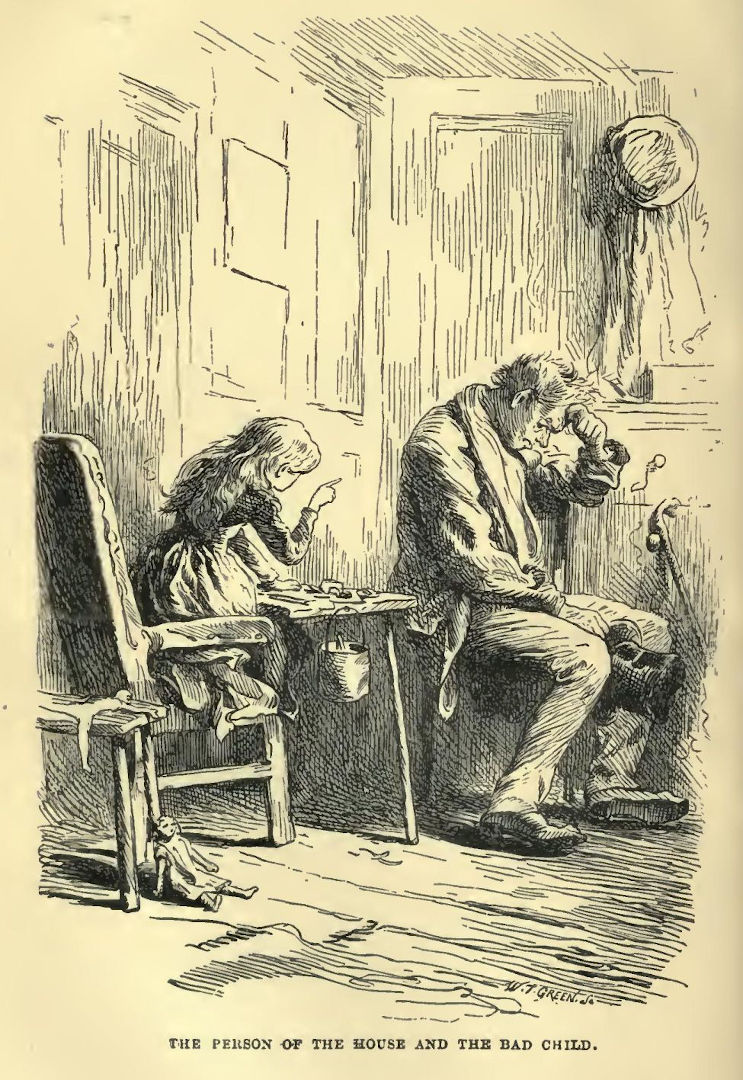
\includegraphics[scale=2.3]{02-02-01}

Chapter 8

IN WHICH AN INNOCENT ELOPEMENT OCCURS


The minion of fortune and the worm of the hour, or in less cutting
language, Nicodemus Boffin, Esquire, the Golden Dustman, had become
as much at home in his eminently aristocratic family mansion as he
was likely ever to be. He could not but feel that, like an eminently
aristocratic family cheese, it was much too large for his wants, and
bred an infinite amount of parasites; but he was content to regard this
drawback on his property as a sort of perpetual Legacy Duty. He felt the
more resigned to it, forasmuch as Mrs Boffin enjoyed herself completely,
and Miss Bella was delighted.

That young lady was, no doubt, an acquisition to the Boffins. She
was far too pretty to be unattractive anywhere, and far too quick of
perception to be below the tone of her new career. Whether it improved
her heart might be a matter of taste that was open to question; but as
touching another matter of taste, its improvement of her appearance and
manner, there could be no question whatever.

And thus it soon came about that Miss Bella began to set Mrs Boffin
right; and even further, that Miss Bella began to feel ill at ease, and
as it were responsible, when she saw Mrs Boffin going wrong. Not that so
sweet a disposition and so sound a nature could ever go very wrong even
among the great visiting authorities who agreed that the Boffins were
‘charmingly vulgar’ (which for certain was not their own case in saying
so), but that when she made a slip on the social ice on which all the
children of Podsnappery, with genteel souls to be saved, are required to
skate in circles, or to slide in long rows, she inevitably tripped Miss
Bella up (so that young lady felt), and caused her to experience great
confusion under the glances of the more skilful performers engaged in
those ice-exercises.

At Miss Bella’s time of life it was not to be expected that she should
examine herself very closely on the congruity or stability of her
position in Mr Boffin’s house. And as she had never been sparing of
complaints of her old home when she had no other to compare it with,
so there was no novelty of ingratitude or disdain in her very much
preferring her new one.

‘An invaluable man is Rokesmith,’ said Mr Boffin, after some two or
three months. ‘But I can’t quite make him out.’

Neither could Bella, so she found the subject rather interesting.

‘He takes more care of my affairs, morning, noon, and night,’ said Mr
Boffin, ‘than fifty other men put together either could or would; and
yet he has ways of his own that are like tying a scaffolding-pole right
across the road, and bringing me up short when I am almost a-walking arm
in arm with him.’

‘May I ask how so, sir?’ inquired Bella.

‘Well, my dear,’ said Mr Boffin, ‘he won’t meet any company here, but
you. When we have visitors, I should wish him to have his regular place
at the table like ourselves; but no, he won’t take it.’

‘If he considers himself above it,’ said Miss Bella, with an airy toss
of her head, ‘I should leave him alone.’

‘It ain’t that, my dear,’ replied Mr Boffin, thinking it over. ‘He don’t
consider himself above it.’

‘Perhaps he considers himself beneath it,’ suggested Bella. ‘If so, he
ought to know best.’

‘No, my dear; nor it ain’t that, neither. No,’ repeated Mr Boffin, with
a shake of his head, after again thinking it over; ‘Rokesmith’s a modest
man, but he don’t consider himself beneath it.’

‘Then what does he consider, sir?’ asked Bella.

‘Dashed if I know!’ said Mr Boffin. ‘It seemed at first as if it
was only Lightwood that he objected to meet. And now it seems to be
everybody, except you.’

Oho! thought Miss Bella. ‘In--deed! That’s it, is it!’ For Mr Mortimer
Lightwood had dined there two or three times, and she had met him
elsewhere, and he had shown her some attention. ‘Rather cool in a
Secretary--and Pa’s lodger--to make me the subject of his jealousy!’

That Pa’s daughter should be so contemptuous of Pa’s lodger was odd;
but there were odder anomalies than that in the mind of the spoilt girl:
spoilt first by poverty, and then by wealth. Be it this history’s part,
however, to leave them to unravel themselves.

‘A little too much, I think,’ Miss Bella reflected scornfully, ‘to
have Pa’s lodger laying claim to me, and keeping eligible people off!
A little too much, indeed, to have the opportunities opened to me by Mr
and Mrs Boffin, appropriated by a mere Secretary and Pa’s lodger!’

Yet it was not so very long ago that Bella had been fluttered by the
discovery that this same Secretary and lodger seem to like her. Ah! but
the eminently aristocratic mansion and Mrs Boffin’s dressmaker had not
come into play then.

In spite of his seemingly retiring manners a very intrusive person, this
Secretary and lodger, in Miss Bella’s opinion. Always a light in his
office-room when we came home from the play or Opera, and he always at
the carriage-door to hand us out. Always a provoking radiance too on
Mrs Boffin’s face, and an abominably cheerful reception of him, as if it
were possible seriously to approve what the man had in his mind!

‘You never charge me, Miss Wilfer,’ said the Secretary, encountering her
by chance alone in the great drawing-room, ‘with commissions for home.
I shall always be happy to execute any commands you may have in that
direction.’

‘Pray what may you mean, Mr Rokesmith?’ inquired Miss Bella, with
languidly drooping eyelids.

‘By home? I mean your father’s house at Holloway.’

She coloured under the retort--so skilfully thrust, that the words
seemed to be merely a plain answer, given in plain good faith--and said,
rather more emphatically and sharply:

‘What commissions and commands are you speaking of?’

‘Only little words of remembrance as I assume you sent somehow or
other,’ replied the Secretary with his former air. ‘It would be a
pleasure to me if you would make me the bearer of them. As you know, I
come and go between the two houses every day.’

‘You needn’t remind me of that, sir.’

She was too quick in this petulant sally against ‘Pa’s lodger’; and she
felt that she had been so when she met his quiet look.

‘They don’t send many--what was your expression?--words of remembrance
to me,’ said Bella, making haste to take refuge in ill-usage.

‘They frequently ask me about you, and I give them such slight
intelligence as I can.’

‘I hope it’s truly given,’ exclaimed Bella.

‘I hope you cannot doubt it, for it would be very much against you, if
you could.’

‘No, I do not doubt it. I deserve the reproach, which is very just
indeed. I beg your pardon, Mr Rokesmith.’

‘I should beg you not to do so, but that it shows you to such admirable
advantage,’ he replied with earnestness. ‘Forgive me; I could not help
saying that. To return to what I have digressed from, let me add that
perhaps they think I report them to you, deliver little messages, and
the like. But I forbear to trouble you, as you never ask me.’

‘I am going, sir,’ said Bella, looking at him as if he had reproved her,
‘to see them tomorrow.’

‘Is that,’ he asked, hesitating, ‘said to me, or to them?’

‘To which you please.’

‘To both? Shall I make it a message?’

‘You can if you like, Mr Rokesmith. Message or no message, I am going to
see them tomorrow.’

‘Then I will tell them so.’

He lingered a moment, as though to give her the opportunity of
prolonging the conversation if she wished. As she remained silent, he
left her. Two incidents of the little interview were felt by Miss Bella
herself, when alone again, to be very curious. The first was, that he
unquestionably left her with a penitent air upon her, and a penitent
feeling in her heart. The second was, that she had not an intention or
a thought of going home, until she had announced it to him as a settled
design.

‘What can I mean by it, or what can he mean by it?’ was her mental
inquiry: ‘He has no right to any power over me, and how do I come to
mind him when I don’t care for him?’

Mrs Boffin, insisting that Bella should make tomorrow’s expedition
in the chariot, she went home in great grandeur. Mrs Wilfer and Miss
Lavinia had speculated much on the probabilities and improbabilities of
her coming in this gorgeous state, and, on beholding the chariot from
the window at which they were secreted to look out for it, agreed
that it must be detained at the door as long as possible, for the
mortification and confusion of the neighbours. Then they repaired to
the usual family room, to receive Miss Bella with a becoming show of
indifference.

The family room looked very small and very mean, and the downward
staircase by which it was attained looked very narrow and very crooked.
The little house and all its arrangements were a poor contrast to the
eminently aristocratic dwelling. ‘I can hardly believe,’ thought Bella,
‘that I ever did endure life in this place!’

Gloomy majesty on the part of Mrs Wilfer, and native pertness on the
part of Lavvy, did not mend the matter. Bella really stood in natural
need of a little help, and she got none.

‘This,’ said Mrs Wilfer, presenting a cheek to be kissed, as sympathetic
and responsive as the back of the bowl of a spoon, ‘is quite an honour!
You will probably find your sister Lavvy grown, Bella.’

‘Ma,’ Miss Lavinia interposed, ‘there can be no objection to your being
aggravating, because Bella richly deserves it; but I really must request
that you will not drag in such ridiculous nonsense as my having grown
when I am past the growing age.’

‘I grew, myself,’ Mrs Wilfer sternly proclaimed, ‘after I was married.’

‘Very well, Ma,’ returned Lavvy, ‘then I think you had much better have
left it alone.’

The lofty glare with which the majestic woman received this answer,
might have embarrassed a less pert opponent, but it had no effect upon
Lavinia: who, leaving her parent to the enjoyment of any amount of
glaring at she might deem desirable under the circumstances, accosted
her sister, undismayed.

‘I suppose you won’t consider yourself quite disgraced, Bella, if I give
you a kiss? Well! And how do you do, Bella? And how are your Boffins?’

‘Peace!’ exclaimed Mrs Wilfer. ‘Hold! I will not suffer this tone of
levity.’

‘My goodness me! How are your Spoffins, then?’ said Lavvy, ‘since Ma so
very much objects to your Boffins.’

‘Impertinent girl! Minx!’ said Mrs Wilfer, with dread severity.

‘I don’t care whether I am a Minx, or a Sphinx,’ returned Lavinia,
coolly, tossing her head; ‘it’s exactly the same thing to me, and I’d
every bit as soon be one as the other; but I know this--I’ll not grow
after I’m married!’

‘You will not? YOU will not?’ repeated Mrs Wilfer, solemnly.

‘No, Ma, I will not. Nothing shall induce me.’

Mrs Wilfer, having waved her gloves, became loftily pathetic.

‘But it was to be expected;’ thus she spake. ‘A child of mine deserts me
for the proud and prosperous, and another child of mine despises me. It
is quite fitting.’

‘Ma,’ Bella struck in, ‘Mr and Mrs Boffin are prosperous, no doubt; but
you have no right to say they are proud. You must know very well that
they are not.’

‘In short, Ma,’ said Lavvy, bouncing over to the enemy without a word
of notice, ‘you must know very well--or if you don’t, more shame for
you!--that Mr and Mrs Boffin are just absolute perfection.’

‘Truly,’ returned Mrs Wilfer, courteously receiving the deserter, ‘it
would seem that we are required to think so. And this, Lavinia, is
my reason for objecting to a tone of levity. Mrs Boffin (of whose
physiognomy I can never speak with the composure I would desire to
preserve), and your mother, are not on terms of intimacy. It is not
for a moment to be supposed that she and her husband dare to presume to
speak of this family as the Wilfers. I cannot therefore condescend to
speak of them as the Boffins. No; for such a tone--call it familiarity,
levity, equality, or what you will--would imply those social
interchanges which do not exist. Do I render myself intelligible?’

Without taking the least notice of this inquiry, albeit delivered in an
imposing and forensic manner, Lavinia reminded her sister, ‘After all,
you know, Bella, you haven’t told us how your Whatshisnames are.’

‘I don’t want to speak of them here,’ replied Bella, suppressing
indignation, and tapping her foot on the floor. ‘They are much too kind
and too good to be drawn into these discussions.’

‘Why put it so?’ demanded Mrs Wilfer, with biting sarcasm. ‘Why adopt a
circuitous form of speech? It is polite and it is obliging; but why do
it? Why not openly say that they are much too kind and too good for US?
We understand the allusion. Why disguise the phrase?’

‘Ma,’ said Bella, with one beat of her foot, ‘you are enough to drive a
saint mad, and so is Lavvy.’

‘Unfortunate Lavvy!’ cried Mrs Wilfer, in a tone of commiseration. ‘She
always comes for it. My poor child!’ But Lavvy, with the suddenness of
her former desertion, now bounced over to the other enemy: very sharply
remarking, ‘Don’t patronize ME, Ma, because I can take care of myself.’

‘I only wonder,’ resumed Mrs Wilfer, directing her observations to her
elder daughter, as safer on the whole than her utterly unmanageable
younger, ‘that you found time and inclination to tear yourself from
Mr and Mrs Boffin, and come to see us at all. I only wonder that our
claims, contending against the superior claims of Mr and Mrs Boffin,
had any weight. I feel I ought to be thankful for gaining so much, in
competition with Mr and Mrs Boffin.’ (The good lady bitterly emphasized
the first letter of the word Boffin, as if it represented her chief
objection to the owners of that name, and as if she could have born
Doffin, Moffin, or Poffin much better.)

‘Ma,’ said Bella, angrily, ‘you force me to say that I am truly sorry I
did come home, and that I never will come home again, except when poor
dear Pa is here. For, Pa is too magnanimous to feel envy and spite
towards my generous friends, and Pa is delicate enough and gentle enough
to remember the sort of little claim they thought I had upon them and
the unusually trying position in which, through no act of my own, I had
been placed. And I always did love poor dear Pa better than all the rest
of you put together, and I always do and I always shall!’

Here Bella, deriving no comfort from her charming bonnet and her elegant
dress, burst into tears.

‘I think, R.W.,’ cried Mrs Wilfer, lifting up her eyes and
apostrophising the air, ‘that if you were present, it would be a
trial to your feelings to hear your wife and the mother of your family
depreciated in your name. But Fate has spared you this, R.W., whatever
it may have thought proper to inflict upon her!’

Here Mrs Wilfer burst into tears.

‘I hate the Boffins!’ protested Miss Lavinia. ‘I don’t care who objects
to their being called the Boffins. I WILL call ‘em the Boffins. The
Boffins, the Boffins, the Boffins! And I say they are mischief-making
Boffins, and I say the Boffins have set Bella against me, and I tell the
Boffins to their faces:’ which was not strictly the fact, but the
young lady was excited: ‘that they are detestable Boffins, disreputable
Boffins, odious Boffins, beastly Boffins. There!’

Here Miss Lavinia burst into tears.

The front garden-gate clanked, and the Secretary was seen coming at a
brisk pace up the steps. ‘Leave Me to open the door to him,’ said Mrs
Wilfer, rising with stately resignation as she shook her head and dried
her eyes; ‘we have at present no stipendiary girl to do so. We have
nothing to conceal. If he sees these traces of emotion on our cheeks,
let him construe them as he may.’

With those words she stalked out. In a few moments she stalked in again,
proclaiming in her heraldic manner, ‘Mr Rokesmith is the bearer of a
packet for Miss Bella Wilfer.’

Mr Rokesmith followed close upon his name, and of course saw what was
amiss. But he discreetly affected to see nothing, and addressed Miss
Bella.

‘Mr Boffin intended to have placed this in the carriage for you
this morning. He wished you to have it, as a little keepsake he had
prepared--it is only a purse, Miss Wilfer--but as he was disappointed in
his fancy, I volunteered to come after you with it.’

Bella took it in her hand, and thanked him.

‘We have been quarrelling here a little, Mr Rokesmith, but not more than
we used; you know our agreeable ways among ourselves. You find me just
going. Good-bye, mamma. Good-bye, Lavvy!’ and with a kiss for each Miss
Bella turned to the door. The Secretary would have attended her, but
Mrs Wilfer advancing and saying with dignity, ‘Pardon me! Permit me to
assert my natural right to escort my child to the equipage which is
in waiting for her,’ he begged pardon and gave place. It was a very
magnificent spectacle indeed, to see Mrs Wilfer throw open the
house-door, and loudly demand with extended gloves, ‘The male domestic
of Mrs Boffin!’ To whom presenting himself, she delivered the brief but
majestic charge, ‘Miss Wilfer. Coming out!’ and so delivered her over,
like a female Lieutenant of the Tower relinquishing a State Prisoner.
The effect of this ceremonial was for some quarter of an hour afterwards
perfectly paralyzing on the neighbours, and was much enhanced by the
worthy lady airing herself for that term in a kind of splendidly serene
trance on the top step.

When Bella was seated in the carriage, she opened the little packet in
her hand. It contained a pretty purse, and the purse contained a bank
note for fifty pounds. ‘This shall be a joyful surprise for poor dear
Pa,’ said Bella, ‘and I’ll take it myself into the City!’

As she was uninformed respecting the exact locality of the place of
business of Chicksey Veneering and Stobbles, but knew it to be near
Mincing Lane, she directed herself to be driven to the corner of that
darksome spot. Thence she despatched ‘the male domestic of Mrs Boffin,’
in search of the counting-house of Chicksey Veneering and Stobbles, with
a message importing that if R. Wilfer could come out, there was a lady
waiting who would be glad to speak with him. The delivery of these
mysterious words from the mouth of a footman caused so great an
excitement in the counting-house, that a youthful scout was instantly
appointed to follow Rumty, observe the lady, and come in with his
report. Nor was the agitation by any means diminished, when the scout
rushed back with the intelligence that the lady was ‘a slap-up gal in a
bang-up chariot.’

Rumty himself, with his pen behind his ear under his rusty hat, arrived
at the carriage-door in a breathless condition, and had been fairly
lugged into the vehicle by his cravat and embraced almost unto choking,
before he recognized his daughter. ‘My dear child!’ he then panted,
incoherently. ‘Good gracious me! What a lovely woman you are! I thought
you had been unkind and forgotten your mother and sister.’

‘I have just been to see them, Pa dear.’

‘Oh! and how--how did you find your mother?’ asked R. W., dubiously.

‘Very disagreeable, Pa, and so was Lavvy.’

‘They are sometimes a little liable to it,’ observed the patient cherub;
‘but I hope you made allowances, Bella, my dear?’

‘No. I was disagreeable too, Pa; we were all of us disagreeable
together. But I want you to come and dine with me somewhere, Pa.’

‘Why, my dear, I have already partaken of a--if one might mention such
an article in this superb chariot--of a--Saveloy,’ replied R. Wilfer,
modestly dropping his voice on the word, as he eyed the canary-coloured
fittings.

‘Oh! That’s nothing, Pa!’

‘Truly, it ain’t as much as one could sometimes wish it to be, my
dear,’ he admitted, drawing his hand across his mouth. ‘Still, when
circumstances over which you have no control, interpose obstacles
between yourself and Small Germans, you can’t do better than bring a
contented mind to hear on’--again dropping his voice in deference to the
chariot--‘Saveloys!’

‘You poor good Pa! Pa, do, I beg and pray, get leave for the rest of the
day, and come and pass it with me!’

‘Well, my dear, I’ll cut back and ask for leave.’

‘But before you cut back,’ said Bella, who had already taken him by the
chin, pulled his hat off, and begun to stick up his hair in her old way,
‘do say that you are sure I am giddy and inconsiderate, but have never
really slighted you, Pa.’

‘My dear, I say it with all my heart. And might I likewise observe,’ her
father delicately hinted, with a glance out at window, ‘that perhaps
it might be calculated to attract attention, having one’s hair publicly
done by a lovely woman in an elegant turn-out in Fenchurch Street?’

Bella laughed and put on his hat again. But when his boyish figure
bobbed away, its shabbiness and cheerful patience smote the tears out
of her eyes. ‘I hate that Secretary for thinking it of me,’ she said to
herself, ‘and yet it seems half true!’

Back came her father, more like a boy than ever, in his release from
school. ‘All right, my dear. Leave given at once. Really very handsomely
done!’

‘Now where can we find some quiet place, Pa, in which I can wait for you
while you go on an errand for me, if I send the carriage away?’

It demanded cogitation. ‘You see, my dear,’ he explained, ‘you really
have become such a very lovely woman, that it ought to be a very quiet
place.’ At length he suggested, ‘Near the garden up by the Trinity House
on Tower Hill.’ So, they were driven there, and Bella dismissed the
chariot; sending a pencilled note by it to Mrs Boffin, that she was with
her father.

‘Now, Pa, attend to what I am going to say, and promise and vow to be
obedient.’

‘I promise and vow, my dear.’

‘You ask no questions. You take this purse; you go to the nearest place
where they keep everything of the very very best, ready made; you buy
and put on, the most beautiful suit of clothes, the most beautiful hat,
and the most beautiful pair of bright boots (patent leather, Pa, mind!)
that are to be got for money; and you come back to me.’

‘But, my dear Bella--’

‘Take care, Pa!’ pointing her forefinger at him, merrily. ‘You have
promised and vowed. It’s perjury, you know.’

There was water in the foolish little fellow’s eyes, but she kissed them
dry (though her own were wet), and he bobbed away again. After half an
hour, he came back, so brilliantly transformed, that Bella was obliged
to walk round him in ecstatic admiration twenty times, before she could
draw her arm through his, and delightedly squeeze it.

‘Now, Pa,’ said Bella, hugging him close, ‘take this lovely woman out to
dinner.’

‘Where shall we go, my dear?’

‘Greenwich!’ said Bella, valiantly. ‘And be sure you treat this lovely
woman with everything of the best.’

While they were going along to take boat, ‘Don’t you wish, my dear,’
said R. W., timidly, ‘that your mother was here?’

‘No, I don’t, Pa, for I like to have you all to myself to-day. I was
always your little favourite at home, and you were always mine. We have
run away together often, before now; haven’t we, Pa?’

‘Ah, to be sure we have! Many a Sunday when your mother was--was a
little liable to it,’ repeating his former delicate expression after
pausing to cough.

‘Yes, and I am afraid I was seldom or never as good as I ought to have
been, Pa. I made you carry me, over and over again, when you should
have made me walk; and I often drove you in harness, when you would much
rather have sat down and read your news-paper: didn’t I?’

‘Sometimes, sometimes. But Lor, what a child you were! What a companion
you were!’

‘Companion? That’s just what I want to be to-day, Pa.’

‘You are safe to succeed, my love. Your brothers and sisters have all
in their turns been companions to me, to a certain extent, but only to a
certain extent. Your mother has, throughout life, been a companion that
any man might--might look up to--and--and commit the sayings of, to
memory--and--form himself upon--if he--’

‘If he liked the model?’ suggested Bella.

‘We-ell, ye-es,’ he returned, thinking about it, not quite satisfied
with the phrase: ‘or perhaps I might say, if it was in him. Supposing,
for instance, that a man wanted to be always marching, he would find
your mother an inestimable companion. But if he had any taste for
walking, or should wish at any time to break into a trot, he might
sometimes find it a little difficult to keep step with your mother.
Or take it this way, Bella,’ he added, after a moment’s reflection;
‘Supposing that a man had to go through life, we won’t say with a
companion, but we’ll say to a tune. Very good. Supposing that the tune
allotted to him was the Dead March in Saul. Well. It would be a very
suitable tune for particular occasions--none better--but it would
be difficult to keep time with in the ordinary run of domestic
transactions. For instance, if he took his supper after a hard day, to
the Dead March in Saul, his food might be likely to sit heavy on him.
Or, if he was at any time inclined to relieve his mind by singing a
comic song or dancing a hornpipe, and was obliged to do it to the Dead
March in Saul, he might find himself put out in the execution of his
lively intentions.’

‘Poor Pa!’ thought Bella, as she hung upon his arm.

‘Now, what I will say for you, my dear,’ the cherub pursued mildly and
without a notion of complaining, ‘is, that you are so adaptable. So
adaptable.’

‘Indeed I am afraid I have shown a wretched temper, Pa. I am afraid
I have been very complaining, and very capricious. I seldom or never
thought of it before. But when I sat in the carriage just now and saw
you coming along the pavement, I reproached myself.’

‘Not at all, my dear. Don’t speak of such a thing.’

A happy and a chatty man was Pa in his new clothes that day. Take it
for all in all, it was perhaps the happiest day he had ever known in his
life; not even excepting that on which his heroic partner had approached
the nuptial altar to the tune of the Dead March in Saul.

The little expedition down the river was delightful, and the little
room overlooking the river into which they were shown for dinner was
delightful. Everything was delightful. The park was delightful, the
punch was delightful, the dishes of fish were delightful, the wine
was delightful. Bella was more delightful than any other item in the
festival; drawing Pa out in the gayest manner; making a point of always
mentioning herself as the lovely woman; stimulating Pa to order things,
by declaring that the lovely woman insisted on being treated with them;
and in short causing Pa to be quite enraptured with the consideration
that he WAS the Pa of such a charming daughter.

And then, as they sat looking at the ships and steamboats making their
way to the sea with the tide that was running down, the lovely woman
imagined all sorts of voyages for herself and Pa. Now, Pa, in the
character of owner of a lumbering square-sailed collier, was tacking
away to Newcastle, to fetch black diamonds to make his fortune with;
now, Pa was going to China in that handsome threemasted ship, to bring
home opium, with which he would for ever cut out Chicksey Veneering
and Stobbles, and to bring home silks and shawls without end for the
decoration of his charming daughter. Now, John Harmon’s disastrous fate
was all a dream, and he had come home and found the lovely woman just
the article for him, and the lovely woman had found him just the article
for her, and they were going away on a trip, in their gallant bark,
to look after their vines, with streamers flying at all points, a band
playing on deck and Pa established in the great cabin. Now, John Harmon
was consigned to his grave again, and a merchant of immense wealth
(name unknown) had courted and married the lovely woman, and he was
so enormously rich that everything you saw upon the river sailing or
steaming belonged to him, and he kept a perfect fleet of yachts for
pleasure, and that little impudent yacht which you saw over there, with
the great white sail, was called The Bella, in honour of his wife, and
she held her state aboard when it pleased her, like a modern Cleopatra.
Anon, there would embark in that troop-ship when she got to Gravesend, a
mighty general, of large property (name also unknown), who wouldn’t
hear of going to victory without his wife, and whose wife was the lovely
woman, and she was destined to become the idol of all the red coats and
blue jackets alow and aloft. And then again: you saw that ship being
towed out by a steam-tug? Well! where did you suppose she was going to?
She was going among the coral reefs and cocoa-nuts and all that sort of
thing, and she was chartered for a fortunate individual of the name
of Pa (himself on board, and much respected by all hands), and she
was going, for his sole profit and advantage, to fetch a cargo of
sweet-smelling woods, the most beautiful that ever were seen, and the
most profitable that ever were heard of; and her cargo would be a great
fortune, as indeed it ought to be: the lovely woman who had purchased
her and fitted her expressly for this voyage, being married to an Indian
Prince, who was a Something-or-Other, and who wore Cashmere shawls all
over himself and diamonds and emeralds blazing in his turban, and was
beautifully coffee-coloured and excessively devoted, though a little too
jealous. Thus Bella ran on merrily, in a manner perfectly enchanting to
Pa, who was as willing to put his head into the Sultan’s tub of water as
the beggar-boys below the window were to put THEIR heads in the mud.

‘I suppose, my dear,’ said Pa after dinner, ‘we may come to the
conclusion at home, that we have lost you for good?’

Bella shook her head. Didn’t know. Couldn’t say. All she was able to
report was, that she was most handsomely supplied with everything she
could possibly want, and that whenever she hinted at leaving Mr and Mrs
Boffin, they wouldn’t hear of it.

‘And now, Pa,’ pursued Bella, ‘I’ll make a confession to you. I am the
most mercenary little wretch that ever lived in the world.’

‘I should hardly have thought it of you, my dear,’ returned her father,
first glancing at himself; and then at the dessert.

‘I understand what you mean, Pa, but it’s not that. It’s not that I care
for money to keep as money, but I do care so much for what it will buy!’

‘Really I think most of us do,’ returned R. W.

‘But not to the dreadful extent that I do, Pa. O-o!’ cried Bella,
screwing the exclamation out of herself with a twist of her dimpled
chin. ‘I AM so mercenary!’

With a wistful glance R. W. said, in default of having anything better
to say: ‘About when did you begin to feel it coming on, my dear?’

‘That’s it, Pa. That’s the terrible part of it. When I was at home, and
only knew what it was to be poor, I grumbled but didn’t so much mind.
When I was at home expecting to be rich, I thought vaguely of all the
great things I would do. But when I had been disappointed of my splendid
fortune, and came to see it from day to day in other hands, and to have
before my eyes what it could really do, then I became the mercenary
little wretch I am.’

‘It’s your fancy, my dear.’

‘I can assure you it’s nothing of the sort, Pa!’ said Bella, nodding at
him, with her very pretty eyebrows raised as high as they would go, and
looking comically frightened. ‘It’s a fact. I am always avariciously
scheming.’

‘Lor! But how?’

‘I’ll tell you, Pa. I don’t mind telling YOU, because we have always
been favourites of each other’s, and because you are not like a Pa, but
more like a sort of a younger brother with a dear venerable chubbiness
on him. And besides,’ added Bella, laughing as she pointed a rallying
finger at his face, ‘because I have got you in my power. This is a
secret expedition. If ever you tell of me, I’ll tell of you. I’ll tell
Ma that you dined at Greenwich.’

‘Well; seriously, my dear,’ observed R. W., with some trepidation of
manner, ‘it might be as well not to mention it.’

‘Aha!’ laughed Bella. ‘I knew you wouldn’t like it, sir! So you keep my
confidence, and I’ll keep yours. But betray the lovely woman, and you
shall find her a serpent. Now, you may give me a kiss, Pa, and I should
like to give your hair a turn, because it has been dreadfully neglected
in my absence.’

R. W. submitted his head to the operator, and the operator went on
talking; at the same time putting separate locks of his hair through
a curious process of being smartly rolled over her two revolving
forefingers, which were then suddenly pulled out of it in opposite
lateral directions. On each of these occasions the patient winced and
winked.

‘I have made up my mind that I must have money, Pa. I feel that I can’t
beg it, borrow it, or steal it; and so I have resolved that I must marry
it.’

R. W. cast up his eyes towards her, as well as he could under the
operating circumstances, and said in a tone of remonstrance, ‘My de-ar
Bella!’

‘Have resolved, I say, Pa, that to get money I must marry money. In
consequence of which, I am always looking out for money to captivate.’

‘My de-a-r Bella!’

‘Yes, Pa, that is the state of the case. If ever there was a mercenary
plotter whose thoughts and designs were always in her mean occupation, I
am the amiable creature. But I don’t care. I hate and detest being
poor, and I won’t be poor if I can marry money. Now you are deliciously
fluffy, Pa, and in a state to astonish the waiter and pay the bill.’

‘But, my dear Bella, this is quite alarming at your age.’

‘I told you so, Pa, but you wouldn’t believe it,’ returned Bella, with a
pleasant childish gravity. ‘Isn’t it shocking?’

‘It would be quite so, if you fully knew what you said, my dear, or
meant it.’

‘Well, Pa, I can only tell you that I mean nothing else. Talk to me of
love!’ said Bella, contemptuously: though her face and figure certainly
rendered the subject no incongruous one. ‘Talk to me of fiery dragons!
But talk to me of poverty and wealth, and there indeed we touch upon
realities.’

‘My De-ar, this is becoming Awful--’ her father was emphatically
beginning: when she stopped him.

‘Pa, tell me. Did you marry money?’

‘You know I didn’t, my dear.’

Bella hummed the Dead March in Saul, and said, after all it signified
very little! But seeing him look grave and downcast, she took him round
the neck and kissed him back to cheerfulness again.

‘I didn’t mean that last touch, Pa; it was only said in joke. Now mind!
You are not to tell of me, and I’ll not tell of you. And more than that;
I promise to have no secrets from you, Pa, and you may make certain
that, whatever mercenary things go on, I shall always tell you all about
them in strict confidence.’

Fain to be satisfied with this concession from the lovely woman, R. W.
rang the bell, and paid the bill. ‘Now, all the rest of this, Pa,’ said
Bella, rolling up the purse when they were alone again, hammering it
small with her little fist on the table, and cramming it into one of the
pockets of his new waistcoat, ‘is for you, to buy presents with for them
at home, and to pay bills with, and to divide as you like, and spend
exactly as you think proper. Last of all take notice, Pa, that it’s
not the fruit of any avaricious scheme. Perhaps if it was, your little
mercenary wretch of a daughter wouldn’t make so free with it!’

After which, she tugged at his coat with both hands, and pulled him all
askew in buttoning that garment over the precious waistcoat pocket, and
then tied her dimples into her bonnet-strings in a very knowing way, and
took him back to London. Arrived at Mr Boffin’s door, she set him with
his back against it, tenderly took him by the ears as convenient handles
for her purpose, and kissed him until he knocked muffled double knocks
at the door with the back of his head. That done, she once more reminded
him of their compact and gaily parted from him.

Not so gaily, however, but that tears filled her eyes as he went away
down the dark street. Not so gaily, but that she several times said,
‘Ah, poor little Pa! Ah, poor dear struggling shabby little Pa!’
before she took heart to knock at the door. Not so gaily, but that the
brilliant furniture seemed to stare her out of countenance as if it
insisted on being compared with the dingy furniture at home. Not so
gaily, but that she fell into very low spirits sitting late in her own
room, and very heartily wept, as she wished, now that the deceased old
John Harmon had never made a will about her, now that the deceased young
John Harmon had lived to marry her. ‘Contradictory things to wish,’ said
Bella, ‘but my life and fortunes are so contradictory altogether that
what can I expect myself to be!’



Chapter 9

IN WHICH THE ORPHAN MAKES HIS WILL


The Secretary, working in the Dismal Swamp betimes next morning, was
informed that a youth waited in the hall who gave the name of Sloppy.
The footman who communicated this intelligence made a decent pause
before uttering the name, to express that it was forced on his
reluctance by the youth in question, and that if the youth had had
the good sense and good taste to inherit some other name it would have
spared the feelings of him the bearer.

‘Mrs Boffin will be very well pleased,’ said the Secretary in a
perfectly composed way. ‘Show him in.’

Mr Sloppy being introduced, remained close to the door: revealing
in various parts of his form many surprising, confounding, and
incomprehensible buttons.

‘I am glad to see you,’ said John Rokesmith, in a cheerful tone of
welcome. ‘I have been expecting you.’

Sloppy explained that he had meant to come before, but that the Orphan
(of whom he made mention as Our Johnny) had been ailing, and he had
waited to report him well.

‘Then he is well now?’ said the Secretary.

‘No he ain’t,’ said Sloppy.

Mr Sloppy having shaken his head to a considerable extent, proceeded
to remark that he thought Johnny ‘must have took ‘em from the Minders.’
Being asked what he meant, he answered, them that come out upon him and
partickler his chest. Being requested to explain himself, he stated that
there was some of ‘em wot you couldn’t kiver with a sixpence. Pressed to
fall back upon a nominative case, he opined that they wos about as
red as ever red could be. ‘But as long as they strikes out’ards, sir,’
continued Sloppy, ‘they ain’t so much. It’s their striking in’ards
that’s to be kep off.’

John Rokesmith hoped the child had had medical attendance? Oh yes, said
Sloppy, he had been took to the doctor’s shop once. And what did the
doctor call it? Rokesmith asked him. After some perplexed reflection,
Sloppy answered, brightening, ‘He called it something as wos wery
long for spots.’ Rokesmith suggested measles. ‘No,’ said Sloppy with
confidence, ‘ever so much longer than THEM, sir!’ (Mr Sloppy was
elevated by this fact, and seemed to consider that it reflected credit
on the poor little patient.)

‘Mrs Boffin will be sorry to hear this,’ said Rokesmith.

‘Mrs Higden said so, sir, when she kep it from her, hoping as Our Johnny
would work round.’

‘But I hope he will?’ said Rokesmith, with a quick turn upon the
messenger.

‘I hope so,’ answered Sloppy. ‘It all depends on their striking
in’ards.’ He then went on to say that whether Johnny had ‘took ‘em’
from the Minders, or whether the Minders had ‘took ’em from Johnny,
the Minders had been sent home and had ‘got ’em.’ Furthermore, that Mrs
Higden’s days and nights being devoted to Our Johnny, who was never out
of her lap, the whole of the mangling arrangements had devolved upon
himself, and he had had ‘rayther a tight time’. The ungainly piece of
honesty beamed and blushed as he said it, quite enraptured with the
remembrance of having been serviceable.

‘Last night,’ said Sloppy, ‘when I was a-turning at the wheel pretty
late, the mangle seemed to go like Our Johnny’s breathing. It begun
beautiful, then as it went out it shook a little and got unsteady, then
as it took the turn to come home it had a rattle-like and lumbered a
bit, then it come smooth, and so it went on till I scarce know’d which
was mangle and which was Our Johnny. Nor Our Johnny, he scarce know’d
either, for sometimes when the mangle lumbers he says, “Me choking,
Granny!” and Mrs Higden holds him up in her lap and says to me “Bide a
bit, Sloppy,” and we all stops together. And when Our Johnny gets his
breathing again, I turns again, and we all goes on together.’

Sloppy had gradually expanded with his description into a stare and a
vacant grin. He now contracted, being silent, into a half-repressed gush
of tears, and, under pretence of being heated, drew the under part of
his sleeve across his eyes with a singularly awkward, laborious, and
roundabout smear.

‘This is unfortunate,’ said Rokesmith. ‘I must go and break it to Mrs
Boffin. Stay you here, Sloppy.’

Sloppy stayed there, staring at the pattern of the paper on the wall,
until the Secretary and Mrs Boffin came back together. And with Mrs
Boffin was a young lady (Miss Bella Wilfer by name) who was better worth
staring at, it occurred to Sloppy, than the best of wall-papering.

‘Ah, my poor dear pretty little John Harmon!’ exclaimed Mrs Boffin.

‘Yes mum,’ said the sympathetic Sloppy.

‘You don’t think he is in a very, very bad way, do you?’ asked the
pleasant creature with her wholesome cordiality.

Put upon his good faith, and finding it in collision with his
inclinations, Sloppy threw back his head and uttered a mellifluous howl,
rounded off with a sniff.

‘So bad as that!’ cried Mrs Boffin. ‘And Betty Higden not to tell me of
it sooner!’

‘I think she might have been mistrustful, mum,’ answered Sloppy,
hesitating.

‘Of what, for Heaven’s sake?’

‘I think she might have been mistrustful, mum,’ returned Sloppy with
submission, ‘of standing in Our Johnny’s light. There’s so much trouble
in illness, and so much expense, and she’s seen such a lot of its being
objected to.’

‘But she never can have thought,’ said Mrs Boffin, ‘that I would grudge
the dear child anything?’

‘No mum, but she might have thought (as a habit-like) of its standing
in Johnny’s light, and might have tried to bring him through it
unbeknownst.’

Sloppy knew his ground well. To conceal herself in sickness, like a
lower animal; to creep out of sight and coil herself away and die; had
become this woman’s instinct. To catch up in her arms the sick child who
was dear to her, and hide it as if it were a criminal, and keep off all
ministration but such as her own ignorant tenderness and patience could
supply, had become this woman’s idea of maternal love, fidelity, and
duty. The shameful accounts we read, every week in the Christian year,
my lords and gentlemen and honourable boards, the infamous records of
small official inhumanity, do not pass by the people as they pass by
us. And hence these irrational, blind, and obstinate prejudices, so
astonishing to our magnificence, and having no more reason in them--God
save the Queen and Confound their politics--no, than smoke has in coming
from fire!

‘It’s not a right place for the poor child to stay in,’ said Mrs Boffin.
‘Tell us, dear Mr Rokesmith, what to do for the best.’

He had already thought what to do, and the consultation was very short.
He could pave the way, he said, in half an hour, and then they would go
down to Brentford. ‘Pray take me,’ said Bella. Therefore a carriage was
ordered, of capacity to take them all, and in the meantime Sloppy
was regaled, feasting alone in the Secretary’s room, with a complete
realization of that fairy vision--meat, beer, vegetables, and pudding.
In consequence of which his buttons became more importunate of public
notice than before, with the exception of two or three about the region
of the waistband, which modestly withdrew into a creasy retirement.

Punctual to the time, appeared the carriage and the Secretary. He sat
on the box, and Mr Sloppy graced the rumble. So, to the Three Magpies as
before: where Mrs Boffin and Miss Bella were handed out, and whence they
all went on foot to Mrs Betty Higden’s.

But, on the way down, they had stopped at a toy-shop, and had bought
that noble charger, a description of whose points and trappings had on
the last occasion conciliated the then worldly-minded orphan, and also a
Noah’s ark, and also a yellow bird with an artificial voice in him,
and also a military doll so well dressed that if he had only been of
life-size his brother-officers in the Guards might never have found him
out. Bearing these gifts, they raised the latch of Betty Higden’s door,
and saw her sitting in the dimmest and furthest corner with poor Johnny
in her lap.

‘And how’s my boy, Betty?’ asked Mrs Boffin, sitting down beside her.

‘He’s bad! He’s bad!’ said Betty. ‘I begin to be afeerd he’ll not be
yours any more than mine. All others belonging to him have gone to
the Power and the Glory, and I have a mind that they’re drawing him to
them--leading him away.’

‘No, no, no,’ said Mrs Boffin.

‘I don’t know why else he clenches his little hand as if it had hold of
a finger that I can’t see. Look at it,’ said Betty, opening the wrappers
in which the flushed child lay, and showing his small right hand lying
closed upon his breast. ‘It’s always so. It don’t mind me.’

‘Is he asleep?’

‘No, I think not. You’re not asleep, my Johnny?’

‘No,’ said Johnny, with a quiet air of pity for himself; and without
opening his eyes.

‘Here’s the lady, Johnny. And the horse.’

Johnny could bear the lady, with complete indifference, but not the
horse. Opening his heavy eyes, he slowly broke into a smile on beholding
that splendid phenomenon, and wanted to take it in his arms. As it was
much too big, it was put upon a chair where he could hold it by the mane
and contemplate it. Which he soon forgot to do.

But, Johnny murmuring something with his eyes closed, and Mrs Boffin
not knowing what, old Betty bent her ear to listen and took pains to
understand. Being asked by her to repeat what he had said, he did so two
or three times, and then it came out that he must have seen more than
they supposed when he looked up to see the horse, for the murmur was,
‘Who is the boofer lady?’ Now, the boofer, or beautiful, lady was Bella;
and whereas this notice from the poor baby would have touched her of
itself; it was rendered more pathetic by the late melting of her heart
to her poor little father, and their joke about the lovely woman. So,
Bella’s behaviour was very tender and very natural when she kneeled on
the brick floor to clasp the child, and when the child, with a child’s
admiration of what is young and pretty, fondled the boofer lady.

‘Now, my good dear Betty,’ said Mrs Boffin, hoping that she saw her
opportunity, and laying her hand persuasively on her arm; ‘we have come
to remove Johnny from this cottage to where he can be taken better care
of.’

Instantly, and before another word could be spoken, the old woman
started up with blazing eyes, and rushed at the door with the sick
child.

‘Stand away from me every one of ye!’ she cried out wildly. ‘I see what
ye mean now. Let me go my way, all of ye. I’d sooner kill the Pretty,
and kill myself!’

‘Stay, stay!’ said Rokesmith, soothing her. ‘You don’t understand.’

‘I understand too well. I know too much about it, sir. I’ve run from
it too many a year. No! Never for me, nor for the child, while there’s
water enough in England to cover us!’

The terror, the shame, the passion of horror and repugnance, firing the
worn face and perfectly maddening it, would have been a quite terrible
sight, if embodied in one old fellow-creature alone. Yet it ‘crops
up’--as our slang goes--my lords and gentlemen and honourable boards, in
other fellow-creatures, rather frequently!

‘It’s been chasing me all my life, but it shall never take me nor mine
alive!’ cried old Betty. ‘I’ve done with ye. I’d have fastened door and
window and starved out, afore I’d ever have let ye in, if I had known
what ye came for!’

But, catching sight of Mrs Boffin’s wholesome face, she relented, and
crouching down by the door and bending over her burden to hush it, said
humbly: ‘Maybe my fears has put me wrong. If they have so, tell me, and
the good Lord forgive me! I’m quick to take this fright, I know, and my
head is summ’at light with wearying and watching.’

‘There, there, there!’ returned Mrs Boffin. ‘Come, come! Say no more of
it, Betty. It was a mistake, a mistake. Any one of us might have made it
in your place, and felt just as you do.’

‘The Lord bless ye!’ said the old woman, stretching out her hand.

‘Now, see, Betty,’ pursued the sweet compassionate soul, holding the
hand kindly, ‘what I really did mean, and what I should have begun by
saying out, if I had only been a little wiser and handier. We want to
move Johnny to a place where there are none but children; a place set
up on purpose for sick children; where the good doctors and nurses pass
their lives with children, talk to none but children, touch none but
children, comfort and cure none but children.’

‘Is there really such a place?’ asked the old woman, with a gaze of
wonder.

‘Yes, Betty, on my word, and you shall see it. If my home was a better
place for the dear boy, I’d take him to it; but indeed indeed it’s not.’

‘You shall take him,’ returned Betty, fervently kissing the comforting
hand, ‘where you will, my deary. I am not so hard, but that I believe
your face and voice, and I will, as long as I can see and hear.’

This victory gained, Rokesmith made haste to profit by it, for he saw
how woefully time had been lost. He despatched Sloppy to bring the
carriage to the door; caused the child to be carefully wrapped up; bade
old Betty get her bonnet on; collected the toys, enabling the little
fellow to comprehend that his treasures were to be transported with
him; and had all things prepared so easily that they were ready for
the carriage as soon as it appeared, and in a minute afterwards were
on their way. Sloppy they left behind, relieving his overcharged breast
with a paroxysm of mangling.

At the Children’s Hospital, the gallant steed, the Noah’s ark, yellow
bird, and the officer in the Guards, were made as welcome as their
child-owner. But the doctor said aside to Rokesmith, ‘This should have
been days ago. Too late!’

However, they were all carried up into a fresh airy room, and there
Johnny came to himself, out of a sleep or a swoon or whatever it was,
to find himself lying in a little quiet bed, with a little platform over
his breast, on which were already arranged, to give him heart and urge
him to cheer up, the Noah’s ark, the noble steed, and the yellow bird;
with the officer in the Guards doing duty over the whole, quite as much
to the satisfaction of his country as if he had been upon Parade. And at
the bed’s head was a coloured picture beautiful to see, representing as
it were another Johnny seated on the knee of some Angel surely who loved
little children. And, marvellous fact, to lie and stare at: Johnny had
become one of a little family, all in little quiet beds (except two
playing dominoes in little arm-chairs at a little table on the hearth):
and on all the little beds were little platforms whereon were to be
seen dolls’ houses, woolly dogs with mechanical barks in them not very
dissimilar from the artificial voice pervading the bowels of the yellow
bird, tin armies, Moorish tumblers, wooden tea things, and the riches of
the earth.

As Johnny murmured something in his placid admiration, the ministering
women at his bed’s head asked him what he said. It seemed that he wanted
to know whether all these were brothers and sisters of his? So they told
him yes. It seemed then, that he wanted to know whether God had brought
them all together there? So they told him yes again. They made out then,
that he wanted to know whether they would all get out of pain? So they
answered yes to that question likewise, and made him understand that the
reply included himself.

Johnny’s powers of sustaining conversation were as yet so very
imperfectly developed, even in a state of health, that in sickness they
were little more than monosyllabic. But, he had to be washed and tended,
and remedies were applied, and though those offices were far, far more
skilfully and lightly done than ever anything had been done for him in
his little life, so rough and short, they would have hurt and tired him
but for an amazing circumstance which laid hold of his attention. This
was no less than the appearance on his own little platform in pairs,
of All Creation, on its way into his own particular ark: the elephant
leading, and the fly, with a diffident sense of his size, politely
bringing up the rear. A very little brother lying in the next bed with a
broken leg, was so enchanted by this spectacle that his delight exalted
its enthralling interest; and so came rest and sleep.

‘I see you are not afraid to leave the dear child here, Betty,’
whispered Mrs Boffin.

‘No, ma’am. Most willingly, most thankfully, with all my heart and
soul.’

So, they kissed him, and left him there, and old Betty was to come back
early in the morning, and nobody but Rokesmith knew for certain how that
the doctor had said, ‘This should have been days ago. Too late!’

But, Rokesmith knowing it, and knowing that his bearing it in mind would
be acceptable thereafter to that good woman who had been the only light
in the childhood of desolate John Harmon dead and gone, resolved that
late at night he would go back to the bedside of John Harmon’s namesake,
and see how it fared with him.

The family whom God had brought together were not all asleep, but were
all quiet. From bed to bed, a light womanly tread and a pleasant fresh
face passed in the silence of the night. A little head would lift itself
up into the softened light here and there, to be kissed as the face went
by--for these little patients are very loving--and would then submit
itself to be composed to rest again. The mite with the broken leg was
restless, and moaned; but after a while turned his face towards Johnny’s
bed, to fortify himself with a view of the ark, and fell asleep. Over
most of the beds, the toys were yet grouped as the children had left
them when they last laid themselves down, and, in their innocent
grotesqueness and incongruity, they might have stood for the children’s
dreams.

The doctor came in too, to see how it fared with Johnny. And he and
Rokesmith stood together, looking down with compassion on him.

‘What is it, Johnny?’ Rokesmith was the questioner, and put an arm round
the poor baby as he made a struggle.

‘Him!’ said the little fellow. ‘Those!’

The doctor was quick to understand children, and, taking the horse,
the ark, the yellow bird, and the man in the Guards, from Johnny’s bed,
softly placed them on that of his next neighbour, the mite with the
broken leg.

With a weary and yet a pleased smile, and with an action as if he
stretched his little figure out to rest, the child heaved his body on
the sustaining arm, and seeking Rokesmith’s face with his lips, said:

‘A kiss for the boofer lady.’

Having now bequeathed all he had to dispose of, and arranged his affairs
in this world, Johnny, thus speaking, left it.



Chapter 10

A SUCCESSOR


Some of the Reverend Frank Milvey’s brethren had found themselves
exceedingly uncomfortable in their minds, because they were required to
bury the dead too hopefully. But, the Reverend Frank, inclining to the
belief that they were required to do one or two other things (say out of
nine-and-thirty) calculated to trouble their consciences rather more if
they would think as much about them, held his peace.

Indeed, the Reverend Frank Milvey was a forbearing man, who noticed many
sad warps and blights in the vineyard wherein he worked, and did not
profess that they made him savagely wise. He only learned that the more
he himself knew, in his little limited human way, the better he could
distantly imagine what Omniscience might know.

Wherefore, if the Reverend Frank had had to read the words that troubled
some of his brethren, and profitably touched innumerable hearts, in
a worse case than Johnny’s, he would have done so out of the pity and
humility of his soul. Reading them over Johnny, he thought of his own
six children, but not of his poverty, and read them with dimmed eyes.
And very seriously did he and his bright little wife, who had been
listening, look down into the small grave and walk home arm-in-arm.

There was grief in the aristocratic house, and there was joy in the
Bower. Mr Wegg argued, if an orphan were wanted, was he not an orphan
himself; and could a better be desired? And why go beating about
Brentford bushes, seeking orphans forsooth who had established no claims
upon you and made no sacrifices for you, when here was an orphan ready
to your hand who had given up in your cause, Miss Elizabeth, Master
George, Aunt Jane, and Uncle Parker?

Mr Wegg chuckled, consequently, when he heard the tidings. Nay, it was
afterwards affirmed by a witness who shall at present be nameless,
that in the seclusion of the Bower he poked out his wooden leg, in the
stage-ballet manner, and executed a taunting or triumphant pirouette on
the genuine leg remaining to him.

John Rokesmith’s manner towards Mrs Boffin at this time, was more the
manner of a young man towards a mother, than that of a Secretary towards
his employer’s wife. It had always been marked by a subdued affectionate
deference that seemed to have sprung up on the very day of his
engagement; whatever was odd in her dress or her ways had seemed to have
no oddity for him; he had sometimes borne a quietly-amused face in her
company, but still it had seemed as if the pleasure her genial temper
and radiant nature yielded him, could have been quite as naturally
expressed in a tear as in a smile. The completeness of his sympathy with
her fancy for having a little John Harmon to protect and rear, he
had shown in every act and word, and now that the kind fancy was
disappointed, he treated it with a manly tenderness and respect for
which she could hardly thank him enough.

‘But I do thank you, Mr Rokesmith,’ said Mrs Boffin, ‘and I thank you
most kindly. You love children.’

‘I hope everybody does.’

‘They ought,’ said Mrs Boffin; ‘but we don’t all of us do what we ought,
do us?’

John Rokesmith replied, ‘Some among us supply the short-comings of the
rest. You have loved children well, Mr Boffin has told me.’

‘Not a bit better than he has, but that’s his way; he puts all the good
upon me. You speak rather sadly, Mr Rokesmith.’

‘Do I?’

‘It sounds to me so. Were you one of many children?’ He shook his head.

‘An only child?’

‘No there was another. Dead long ago.’

‘Father or mother alive?’

‘Dead.’--

‘And the rest of your relations?’

‘Dead--if I ever had any living. I never heard of any.’

At this point of the dialogue Bella came in with a light step. She
paused at the door a moment, hesitating whether to remain or retire;
perplexed by finding that she was not observed.

‘Now, don’t mind an old lady’s talk,’ said Mrs Boffin, ‘but tell me. Are
you quite sure, Mr Rokesmith, that you have never had a disappointment
in love?’

‘Quite sure. Why do you ask me?’

‘Why, for this reason. Sometimes you have a kind of kept-down manner
with you, which is not like your age. You can’t be thirty?’

‘I am not yet thirty.’

Deeming it high time to make her presence known, Bella coughed here to
attract attention, begged pardon, and said she would go, fearing that
she interrupted some matter of business.

‘No, don’t go,’ rejoined Mrs Boffin, ‘because we are coming to business,
instead of having begun it, and you belong to it as much now, my dear
Bella, as I do. But I want my Noddy to consult with us. Would somebody
be so good as find my Noddy for me?’

Rokesmith departed on that errand, and presently returned accompanied by
Mr Boffin at his jog-trot. Bella felt a little vague trepidation as to
the subject-matter of this same consultation, until Mrs Boffin announced
it.

‘Now, you come and sit by me, my dear,’ said that worthy soul, taking
her comfortable place on a large ottoman in the centre of the room,
and drawing her arm through Bella’s; ‘and Noddy, you sit here, and Mr
Rokesmith you sit there. Now, you see, what I want to talk about, is
this. Mr and Mrs Milvey have sent me the kindest note possible (which
Mr Rokesmith just now read to me out aloud, for I ain’t good at
handwritings), offering to find me another little child to name and
educate and bring up. Well. This has set me thinking.’

[‘And she is a steam-ingein at it,’ murmured Mr Boffin, in an admiring
parenthesis, ‘when she once begins. It mayn’t be so easy to start her;
but once started, she’s a ingein.’)

‘--This has set me thinking, I say,’ repeated Mrs Boffin, cordially
beaming under the influence of her husband’s compliment, ‘and I have
thought two things. First of all, that I have grown timid of reviving
John Harmon’s name. It’s an unfortunate name, and I fancy I should
reproach myself if I gave it to another dear child, and it proved again
unlucky.’

‘Now, whether,’ said Mr Boffin, gravely propounding a case for his
Secretary’s opinion; ‘whether one might call that a superstition?’

‘It is a matter of feeling with Mrs Boffin,’ said Rokesmith, gently.
‘The name has always been unfortunate. It has now this new unfortunate
association connected with it. The name has died out. Why revive it?
Might I ask Miss Wilfer what she thinks?’

‘It has not been a fortunate name for me,’ said Bella, colouring--‘or
at least it was not, until it led to my being here--but that is not the
point in my thoughts. As we had given the name to the poor child, and as
the poor child took so lovingly to me, I think I should feel jealous of
calling another child by it. I think I should feel as if the name had
become endeared to me, and I had no right to use it so.’

‘And that’s your opinion?’ remarked Mr Boffin, observant of the
Secretary’s face and again addressing him.

‘I say again, it is a matter of feeling,’ returned the Secretary. ‘I
think Miss Wilfer’s feeling very womanly and pretty.’

‘Now, give us your opinion, Noddy,’ said Mrs Boffin.

‘My opinion, old lady,’ returned the Golden Dustman, ‘is your opinion.’

‘Then,’ said Mrs Boffin, ‘we agree not to revive John Harmon’s name, but
to let it rest in the grave. It is, as Mr Rokesmith says, a matter of
feeling, but Lor how many matters ARE matters of feeling! Well; and so
I come to the second thing I have thought of. You must know, Bella,
my dear, and Mr Rokesmith, that when I first named to my husband my
thoughts of adopting a little orphan boy in remembrance of John Harmon,
I further named to my husband that it was comforting to think that how
the poor boy would be benefited by John’s own money, and protected from
John’s own forlornness.’

‘Hear, hear!’ cried Mr Boffin. ‘So she did. Ancoar!’

‘No, not Ancoar, Noddy, my dear,’ returned Mrs Boffin, ‘because I am
going to say something else. I meant that, I am sure, as much as
I still mean it. But this little death has made me ask myself the
question, seriously, whether I wasn’t too bent upon pleasing myself.
Else why did I seek out so much for a pretty child, and a child quite to
my liking? Wanting to do good, why not do it for its own sake, and put
my tastes and likings by?’

‘Perhaps,’ said Bella; and perhaps she said it with some little
sensitiveness arising out of those old curious relations of hers towards
the murdered man; ‘perhaps, in reviving the name, you would not have
liked to give it to a less interesting child than the original. He
interested you very much.’

‘Well, my dear,’ returned Mrs Boffin, giving her a squeeze, ‘it’s kind
of you to find that reason out, and I hope it may have been so, and
indeed to a certain extent I believe it was so, but I am afraid not to
the whole extent. However, that don’t come in question now, because we
have done with the name.’

‘Laid it up as a remembrance,’ suggested Bella, musingly.

‘Much better said, my dear; laid it up as a remembrance. Well then; I
have been thinking if I take any orphan to provide for, let it not be
a pet and a plaything for me, but a creature to be helped for its own
sake.’

‘Not pretty then?’ said Bella.

‘No,’ returned Mrs Boffin, stoutly.

‘Nor prepossessing then?’ said Bella.

‘No,’ returned Mrs Boffin. ‘Not necessarily so. That’s as it may happen.
A well-disposed boy comes in my way who may be even a little wanting in
such advantages for getting on in life, but is honest and industrious
and requires a helping hand and deserves it. If I am very much in
earnest and quite determined to be unselfish, let me take care of HIM.’

Here the footman whose feelings had been hurt on the former occasion,
appeared, and crossing to Rokesmith apologetically announced the
objectionable Sloppy.

The four members of Council looked at one another, and paused. ‘Shall he
be brought here, ma’am?’ asked Rokesmith.

‘Yes,’ said Mrs Boffin. Whereupon the footman disappeared, reappeared
presenting Sloppy, and retired much disgusted.

The consideration of Mrs Boffin had clothed Mr Sloppy in a suit of
black, on which the tailor had received personal directions from
Rokesmith to expend the utmost cunning of his art, with a view to the
concealment of the cohering and sustaining buttons. But, so much
more powerful were the frailties of Sloppy’s form than the strongest
resources of tailoring science, that he now stood before the Council,
a perfect Argus in the way of buttons: shining and winking and gleaming
and twinkling out of a hundred of those eyes of bright metal, at the
dazzled spectators. The artistic taste of some unknown hatter had
furnished him with a hatband of wholesale capacity which was fluted
behind, from the crown of his hat to the brim, and terminated in a black
bunch, from which the imagination shrunk discomfited and the reason
revolted. Some special powers with which his legs were endowed, had
already hitched up his glossy trousers at the ankles, and bagged them at
the knees; while similar gifts in his arms had raised his coat-sleeves
from his wrists and accumulated them at his elbows. Thus set forth, with
the additional embellishments of a very little tail to his coat, and a
yawning gulf at his waistband, Sloppy stood confessed.

‘And how is Betty, my good fellow?’ Mrs Boffin asked him.

‘Thankee, mum,’ said Sloppy, ‘she do pretty nicely, and sending her
dooty and many thanks for the tea and all faviours and wishing to know
the family’s healths.’

‘Have you just come, Sloppy?’

‘Yes, mum.’

‘Then you have not had your dinner yet?’

‘No, mum. But I mean to it. For I ain’t forgotten your handsome orders
that I was never to go away without having had a good ‘un off of meat
and beer and pudding--no: there was four of ‘em, for I reckoned ‘em
up when I had ‘em; meat one, beer two, vegetables three, and which was
four?--Why, pudding, HE was four!’ Here Sloppy threw his head back,
opened his mouth wide, and laughed rapturously.

‘How are the two poor little Minders?’ asked Mrs Boffin.

‘Striking right out, mum, and coming round beautiful.’

Mrs Boffin looked on the other three members of Council, and then said,
beckoning with her finger:

‘Sloppy.’

‘Yes, mum.’

‘Come forward, Sloppy. Should you like to dine here every day?’

‘Off of all four on ‘em, mum? O mum!’ Sloppy’s feelings obliged him to
squeeze his hat, and contract one leg at the knee.

‘Yes. And should you like to be always taken care of here, if you were
industrious and deserving?’

‘Oh, mum!--But there’s Mrs Higden,’ said Sloppy, checking himself in his
raptures, drawing back, and shaking his head with very serious meaning.
‘There’s Mrs Higden. Mrs Higden goes before all. None can ever be better
friends to me than Mrs Higden’s been. And she must be turned for, must
Mrs Higden. Where would Mrs Higden be if she warn’t turned for!’ At the
mere thought of Mrs Higden in this inconceivable affliction, Mr Sloppy’s
countenance became pale, and manifested the most distressful emotions.

‘You are as right as right can be, Sloppy,’ said Mrs Boffin ‘and far be
it from me to tell you otherwise. It shall be seen to. If Betty Higden
can be turned for all the same, you shall come here and be taken care of
for life, and be made able to keep her in other ways than the turning.’

‘Even as to that, mum,’ answered the ecstatic Sloppy, ‘the turning might
be done in the night, don’t you see? I could be here in the day, and
turn in the night. I don’t want no sleep, I don’t. Or even if I any ways
should want a wink or two,’ added Sloppy, after a moment’s apologetic
reflection, ‘I could take ‘em turning. I’ve took ‘em turning many a
time, and enjoyed ‘em wonderful!’

On the grateful impulse of the moment, Mr Sloppy kissed Mrs Boffin’s
hand, and then detaching himself from that good creature that he might
have room enough for his feelings, threw back his head, opened his mouth
wide, and uttered a dismal howl. It was creditable to his tenderness of
heart, but suggested that he might on occasion give some offence to the
neighbours: the rather, as the footman looked in, and begged pardon,
finding he was not wanted, but excused himself; on the ground ‘that he
thought it was Cats.’



Chapter 11

SOME AFFAIRS OF THE HEART


Little Miss Peecher, from her little official dwelling-house, with its
little windows like the eyes in needles, and its little doors like the
covers of school-books, was very observant indeed of the object of her
quiet affections. Love, though said to be afflicted with blindness, is
a vigilant watchman, and Miss Peecher kept him on double duty over Mr
Bradley Headstone. It was not that she was naturally given to playing
the spy--it was not that she was at all secret, plotting, or mean--it
was simply that she loved the irresponsive Bradley with all the
primitive and homely stock of love that had never been examined or
certificated out of her. If her faithful slate had had the latent
qualities of sympathetic paper, and its pencil those of invisible ink,
many a little treatise calculated to astonish the pupils would have come
bursting through the dry sums in school-time under the warming influence
of Miss Peecher’s bosom. For, oftentimes when school was not, and her
calm leisure and calm little house were her own, Miss Peecher would
commit to the confidential slate an imaginary description of how, upon
a balmy evening at dusk, two figures might have been observed in the
market-garden ground round the corner, of whom one, being a manly form,
bent over the other, being a womanly form of short stature and some
compactness, and breathed in a low voice the words, ‘Emma Peecher, wilt
thou be my own?’ after which the womanly form’s head reposed upon the
manly form’s shoulder, and the nightingales tuned up. Though all unseen,
and unsuspected by the pupils, Bradley Headstone even pervaded the
school exercises. Was Geography in question? He would come triumphantly
flying out of Vesuvius and Aetna ahead of the lava, and would boil
unharmed in the hot springs of Iceland, and would float majestically
down the Ganges and the Nile. Did History chronicle a king of men?
Behold him in pepper-and-salt pantaloons, with his watch-guard round
his neck. Were copies to be written? In capital B’s and H’s most of the
girls under Miss Peecher’s tuition were half a year ahead of every other
letter in the alphabet. And Mental Arithmetic, administered by Miss
Peecher, often devoted itself to providing Bradley Headstone with a
wardrobe of fabulous extent: fourscore and four neck-ties at two and
ninepence-halfpenny, two gross of silver watches at four pounds fifteen
and sixpence, seventy-four black hats at eighteen shillings; and many
similar superfluities.

The vigilant watchman, using his daily opportunities of turning his eyes
in Bradley’s direction, soon apprized Miss Peecher that Bradley was more
preoccupied than had been his wont, and more given to strolling about
with a downcast and reserved face, turning something difficult in his
mind that was not in the scholastic syllabus. Putting this and that
together--combining under the head ‘this,’ present appearances and the
intimacy with Charley Hexam, and ranging under the head ‘that’ the
visit to his sister, the watchman reported to Miss Peecher his strong
suspicions that the sister was at the bottom of it.

‘I wonder,’ said Miss Peecher, as she sat making up her weekly report on
a half-holiday afternoon, ‘what they call Hexam’s sister?’

Mary Anne, at her needlework, attendant and attentive, held her arm up.

‘Well, Mary Anne?’

‘She is named Lizzie, ma’am.’

‘She can hardly be named Lizzie, I think, Mary Anne,’ returned Miss
Peecher, in a tunefully instructive voice. ‘Is Lizzie a Christian name,
Mary Anne?’

Mary Anne laid down her work, rose, hooked herself behind, as being
under catechization, and replied: ‘No, it is a corruption, Miss
Peecher.’

‘Who gave her that name?’ Miss Peecher was going on, from the mere force
of habit, when she checked herself; on Mary Anne’s evincing theological
impatience to strike in with her godfathers and her godmothers, and
said: ‘I mean of what name is it a corruption?’

‘Elizabeth, or Eliza, Miss Peecher.’

‘Right, Mary Anne. Whether there were any Lizzies in the early Christian
Church must be considered very doubtful, very doubtful.’ Miss Peecher
was exceedingly sage here. ‘Speaking correctly, we say, then, that
Hexam’s sister is called Lizzie; not that she is named so. Do we not,
Mary Anne?’

‘We do, Miss Peecher.’

‘And where,’ pursued Miss Peecher, complacent in her little transparent
fiction of conducting the examination in a semiofficial manner for Mary
Anne’s benefit, not her own, ‘where does this young woman, who is called
but not named Lizzie, live? Think, now, before answering.’

‘In Church Street, Smith Square, by Mill Bank, ma’am.’

‘In Church Street, Smith Square, by Mill Bank,’ repeated Miss Peecher,
as if possessed beforehand of the book in which it was written. Exactly
so. And what occupation does this young woman pursue, Mary Anne? Take
time.’

‘She has a place of trust at an outfitter’s in the City, ma’am.’

‘Oh!’ said Miss Peecher, pondering on it; but smoothly added, in a
confirmatory tone, ‘At an outfitter’s in the City. Ye-es?’

‘And Charley--’ Mary Anne was proceeding, when Miss Peecher stared.

‘I mean Hexam, Miss Peecher.’

‘I should think you did, Mary Anne. I am glad to hear you do. And
Hexam--’

‘Says,’ Mary Anne went on, ‘that he is not pleased with his sister, and
that his sister won’t be guided by his advice, and persists in being
guided by somebody else’s; and that--’

‘Mr Headstone coming across the garden!’ exclaimed Miss Peecher, with a
flushed glance at the looking-glass. ‘You have answered very well, Mary
Anne. You are forming an excellent habit of arranging your thoughts
clearly. That will do.’

The discreet Mary Anne resumed her seat and her silence, and stitched,
and stitched, and was stitching when the schoolmaster’s shadow came in
before him, announcing that he might be instantly expected.

‘Good evening, Miss Peecher,’ he said, pursuing the shadow, and taking
its place.

‘Good evening, Mr Headstone. Mary Anne, a chair.’

‘Thank you,’ said Bradley, seating himself in his constrained manner.
‘This is but a flying visit. I have looked in, on my way, to ask a
kindness of you as a neighbour.’

‘Did you say on your way, Mr Headstone?’ asked Miss Peecher.

‘On my way to--where I am going.’

‘Church Street, Smith Square, by Mill Bank,’ repeated Miss Peecher, in
her own thoughts.

‘Charley Hexam has gone to get a book or two he wants, and will probably
be back before me. As we leave my house empty, I took the liberty of
telling him I would leave the key here. Would you kindly allow me to do
so?’

‘Certainly, Mr Headstone. Going for an evening walk, sir?’

‘Partly for a walk, and partly for--on business.’

‘Business in Church Street, Smith Square, by Mill Bank,’ repeated Miss
Peecher to herself.

‘Having said which,’ pursued Bradley, laying his door-key on the table,
‘I must be already going. There is nothing I can do for you, Miss
Peecher?’

‘Thank you, Mr Headstone. In which direction?’

‘In the direction of Westminster.’

‘Mill Bank,’ Miss Peecher repeated in her own thoughts once again. ‘No,
thank you, Mr Headstone; I’ll not trouble you.’

‘You couldn’t trouble me,’ said the schoolmaster.

‘Ah!’ returned Miss Peecher, though not aloud; ‘but you can trouble
ME!’ And for all her quiet manner, and her quiet smile, she was full of
trouble as he went his way.

She was right touching his destination. He held as straight a course
for the house of the dolls’ dressmaker as the wisdom of his ancestors,
exemplified in the construction of the intervening streets, would let
him, and walked with a bent head hammering at one fixed idea. It had
been an immoveable idea since he first set eyes upon her. It seemed to
him as if all that he could suppress in himself he had suppressed, as
if all that he could restrain in himself he had restrained, and the time
had come--in a rush, in a moment--when the power of self-command had
departed from him. Love at first sight is a trite expression quite
sufficiently discussed; enough that in certain smouldering natures like
this man’s, that passion leaps into a blaze, and makes such head as fire
does in a rage of wind, when other passions, but for its mastery, could
be held in chains. As a multitude of weak, imitative natures are
always lying by, ready to go mad upon the next wrong idea that may be
broached--in these times, generally some form of tribute to Somebody
for something that never was done, or, if ever done, that was done by
Somebody Else--so these less ordinary natures may lie by for years,
ready on the touch of an instant to burst into flame.

The schoolmaster went his way, brooding and brooding, and a sense of
being vanquished in a struggle might have been pieced out of his worried
face. Truly, in his breast there lingered a resentful shame to find
himself defeated by this passion for Charley Hexam’s sister, though in
the very self-same moments he was concentrating himself upon the object
of bringing the passion to a successful issue.

He appeared before the dolls’ dressmaker, sitting alone at her work.
‘Oho!’ thought that sharp young personage, ‘it’s you, is it? I know your
tricks and your manners, my friend!’

‘Hexam’s sister,’ said Bradley Headstone, ‘is not come home yet?’

‘You are quite a conjuror,’ returned Miss Wren.

‘I will wait, if you please, for I want to speak to her.’

‘Do you?’ returned Miss Wren. ‘Sit down. I hope it’s mutual.’ Bradley
glanced distrustfully at the shrewd face again bending over the work,
and said, trying to conquer doubt and hesitation:

‘I hope you don’t imply that my visit will be unacceptable to Hexam’s
sister?’

‘There! Don’t call her that. I can’t bear you to call her that,’
returned Miss Wren, snapping her fingers in a volley of impatient snaps,
‘for I don’t like Hexam.’

‘Indeed?’

‘No.’ Miss Wren wrinkled her nose, to express dislike. ‘Selfish. Thinks
only of himself. The way with all of you.’

‘The way with all of us? Then you don’t like ME?’

‘So-so,’ replied Miss Wren, with a shrug and a laugh. ‘Don’t know much
about you.’

‘But I was not aware it was the way with all of us,’ said Bradley,
returning to the accusation, a little injured. ‘Won’t you say, some of
us?’

‘Meaning,’ returned the little creature, ‘every one of you, but you.
Hah! Now look this lady in the face. This is Mrs Truth. The Honourable.
Full-dressed.’

Bradley glanced at the doll she held up for his observation--which had
been lying on its face on her bench, while with a needle and thread she
fastened the dress on at the back--and looked from it to her.

‘I stand the Honourable Mrs T. on my bench in this corner against the
wall, where her blue eyes can shine upon you,’ pursued Miss Wren, doing
so, and making two little dabs at him in the air with her needle, as
if she pricked him with it in his own eyes; ‘and I defy you to tell me,
with Mrs T. for a witness, what you have come here for.’

‘To see Hexam’s sister.’

‘You don’t say so!’ retorted Miss Wren, hitching her chin. ‘But on whose
account?’

‘Her own.’

‘O Mrs T.!’ exclaimed Miss Wren. ‘You hear him!’

‘To reason with her,’ pursued Bradley, half humouring what was present,
and half angry with what was not present; ‘for her own sake.’

‘Oh Mrs T.!’ exclaimed the dressmaker.

‘For her own sake,’ repeated Bradley, warming, ‘and for her brother’s,
and as a perfectly disinterested person.’

‘Really, Mrs T.,’ remarked the dressmaker, ‘since it comes to this, we
must positively turn you with your face to the wall.’ She had hardly
done so, when Lizzie Hexam arrived, and showed some surprise on seeing
Bradley Headstone there, and Jenny shaking her little fist at him close
before her eyes, and the Honourable Mrs T. with her face to the wall.

‘Here’s a perfectly disinterested person, Lizzie dear,’ said the knowing
Miss Wren, ‘come to talk with you, for your own sake and your brother’s.
Think of that. I am sure there ought to be no third party present at
anything so very kind and so very serious; and so, if you’ll remove the
third party upstairs, my dear, the third party will retire.’

Lizzie took the hand which the dolls’ dressmaker held out to her for
the purpose of being supported away, but only looked at her with an
inquiring smile, and made no other movement.

‘The third party hobbles awfully, you know, when she’s left to herself;’
said Miss Wren, ‘her back being so bad, and her legs so queer; so she
can’t retire gracefully unless you help her, Lizzie.’

‘She can do no better than stay where she is,’ returned Lizzie,
releasing the hand, and laying her own lightly on Miss Jenny’s curls.
And then to Bradley: ‘From Charley, sir?’

In an irresolute way, and stealing a clumsy look at her, Bradley rose to
place a chair for her, and then returned to his own.

‘Strictly speaking,’ said he, ‘I come from Charley, because I left him
only a little while ago; but I am not commissioned by Charley. I come of
my own spontaneous act.’

With her elbows on her bench, and her chin upon her hands, Miss Jenny
Wren sat looking at him with a watchful sidelong look. Lizzie, in her
different way, sat looking at him too.

‘The fact is,’ began Bradley, with a mouth so dry that he had some
difficulty in articulating his words: the consciousness of which
rendered his manner still more ungainly and undecided; ‘the truth is,
that Charley, having no secrets from me (to the best of my belief), has
confided the whole of this matter to me.’

He came to a stop, and Lizzie asked: ‘what matter, sir?’

‘I thought,’ returned the schoolmaster, stealing another look at her,
and seeming to try in vain to sustain it; for the look dropped as it
lighted on her eyes, ‘that it might be so superfluous as to be almost
impertinent, to enter upon a definition of it. My allusion was to this
matter of your having put aside your brother’s plans for you, and
given the preference to those of Mr--I believe the name is Mr Eugene
Wrayburn.’

He made this point of not being certain of the name, with another uneasy
look at her, which dropped like the last.

Nothing being said on the other side, he had to begin again, and began
with new embarrassment.

‘Your brother’s plans were communicated to me when he first had them in
his thoughts. In point of fact he spoke to me about them when I was
last here--when we were walking back together, and when I--when the
impression was fresh upon me of having seen his sister.’

There might have been no meaning in it, but the little dressmaker here
removed one of her supporting hands from her chin, and musingly turned
the Honourable Mrs T. with her face to the company. That done, she fell
into her former attitude.

‘I approved of his idea,’ said Bradley, with his uneasy look wandering
to the doll, and unconsciously resting there longer than it had
rested on Lizzie, ‘both because your brother ought naturally to be the
originator of any such scheme, and because I hoped to be able to promote
it. I should have had inexpressible pleasure, I should have taken
inexpressible interest, in promoting it. Therefore I must acknowledge
that when your brother was disappointed, I too was disappointed. I wish
to avoid reservation or concealment, and I fully acknowledge that.’

He appeared to have encouraged himself by having got so far. At all
events he went on with much greater firmness and force of emphasis:
though with a curious disposition to set his teeth, and with a curious
tight-screwing movement of his right hand in the clenching palm of his
left, like the action of one who was being physically hurt, and was
unwilling to cry out.

‘I am a man of strong feelings, and I have strongly felt this
disappointment. I do strongly feel it. I don’t show what I feel; some
of us are obliged habitually to keep it down. To keep it down. But to
return to your brother. He has taken the matter so much to heart that
he has remonstrated (in my presence he remonstrated) with Mr Eugene
Wrayburn, if that be the name. He did so, quite ineffectually. As any
one not blinded to the real character of Mr--Mr Eugene Wrayburn--would
readily suppose.’

He looked at Lizzie again, and held the look. And his face turned from
burning red to white, and from white back to burning red, and so for the
time to lasting deadly white.

‘Finally, I resolved to come here alone, and appeal to you. I resolved
to come here alone, and entreat you to retract the course you have
chosen, and instead of confiding in a mere stranger--a person of most
insolent behaviour to your brother and others--to prefer your brother
and your brother’s friend.’

Lizzie Hexam had changed colour when those changes came over him, and
her face now expressed some anger, more dislike, and even a touch of
fear. But she answered him very steadily.

‘I cannot doubt, Mr Headstone, that your visit is well meant. You have
been so good a friend to Charley that I have no right to doubt it. I
have nothing to tell Charley, but that I accepted the help to which he
so much objects before he made any plans for me; or certainly before I
knew of any. It was considerately and delicately offered, and there were
reasons that had weight with me which should be as dear to Charley as to
me. I have no more to say to Charley on this subject.’

His lips trembled and stood apart, as he followed this repudiation of
himself; and limitation of her words to her brother.

‘I should have told Charley, if he had come to me,’ she resumed, as
though it were an after-thought, ‘that Jenny and I find our teacher very
able and very patient, and that she takes great pains with us. So much
so, that we have said to her we hope in a very little while to be able
to go on by ourselves. Charley knows about teachers, and I should also
have told him, for his satisfaction, that ours comes from an institution
where teachers are regularly brought up.’

‘I should like to ask you,’ said Bradley Headstone, grinding his words
slowly out, as though they came from a rusty mill; ‘I should like to
ask you, if I may without offence, whether you would have objected--no;
rather, I should like to say, if I may without offence, that I wish I
had had the opportunity of coming here with your brother and devoting my
poor abilities and experience to your service.’

‘Thank you, Mr Headstone.’

‘But I fear,’ he pursued, after a pause, furtively wrenching at the seat
of his chair with one hand, as if he would have wrenched the chair to
pieces, and gloomily observing her while her eyes were cast down, ‘that
my humble services would not have found much favour with you?’

She made no reply, and the poor stricken wretch sat contending with
himself in a heat of passion and torment. After a while he took out his
handkerchief and wiped his forehead and hands.

‘There is only one thing more I had to say, but it is the most
important. There is a reason against this matter, there is a personal
relation concerned in this matter, not yet explained to you. It might--I
don’t say it would--it might--induce you to think differently. To
proceed under the present circumstances is out of the question. Will you
please come to the understanding that there shall be another interview
on the subject?’

‘With Charley, Mr Headstone?’

‘With--well,’ he answered, breaking off, ‘yes! Say with him too.
Will you please come to the understanding that there must be another
interview under more favourable circumstances, before the whole case can
be submitted?’

‘I don’t,’ said Lizzie, shaking her head, ‘understand your meaning, Mr
Headstone.’

‘Limit my meaning for the present,’ he interrupted, ‘to the whole case
being submitted to you in another interview.’

‘What case, Mr Headstone? What is wanting to it?’

‘You--you shall be informed in the other interview.’ Then he said, as
if in a burst of irrepressible despair, ‘I--I leave it all incomplete!
There is a spell upon me, I think!’ And then added, almost as if he
asked for pity, ‘Good-night!’

He held out his hand. As she, with manifest hesitation, not to say
reluctance, touched it, a strange tremble passed over him, and his face,
so deadly white, was moved as by a stroke of pain. Then he was gone.

The dolls’ dressmaker sat with her attitude unchanged, eyeing the door
by which he had departed, until Lizzie pushed her bench aside and sat
down near her. Then, eyeing Lizzie as she had previously eyed Bradley
and the door, Miss Wren chopped that very sudden and keen chop in which
her jaws sometimes indulged, leaned back in her chair with folded arms,
and thus expressed herself:

‘Humph! If he--I mean, of course, my dear, the party who is coming to
court me when the time comes--should be THAT sort of man, he may spare
himself the trouble. HE wouldn’t do to be trotted about and made useful.
He’d take fire and blow up while he was about it.’

‘And so you would be rid of him,’ said Lizzie, humouring her.

‘Not so easily,’ returned Miss Wren. ‘He wouldn’t blow up alone. He’d
carry me up with him. I know his tricks and his manners.’

‘Would he want to hurt you, do you mean?’ asked Lizzie.

‘Mightn’t exactly want to do it, my dear,’ returned Miss Wren; ‘but a
lot of gunpowder among lighted lucifer-matches in the next room might
almost as well be here.’

‘He is a very strange man,’ said Lizzie, thoughtfully.

‘I wish he was so very strange a man as to be a total stranger,’
answered the sharp little thing.

It being Lizzie’s regular occupation when they were alone of an evening
to brush out and smooth the long fair hair of the dolls’ dressmaker, she
unfastened a ribbon that kept it back while the little creature was at
her work, and it fell in a beautiful shower over the poor shoulders that
were much in need of such adorning rain. ‘Not now, Lizzie, dear,’ said
Jenny; ‘let us have a talk by the fire.’ With those words, she in her
turn loosened her friend’s dark hair, and it dropped of its own weight
over her bosom, in two rich masses. Pretending to compare the colours
and admire the contrast, Jenny so managed a mere touch or two of her
nimble hands, as that she herself laying a cheek on one of the dark
folds, seemed blinded by her own clustering curls to all but the fire,
while the fine handsome face and brow of Lizzie were revealed without
obstruction in the sombre light.

‘Let us have a talk,’ said Jenny, ‘about Mr Eugene Wrayburn.’

Something sparkled down among the fair hair resting on the dark hair;
and if it were not a star--which it couldn’t be--it was an eye; and
if it were an eye, it was Jenny Wren’s eye, bright and watchful as the
bird’s whose name she had taken.

‘Why about Mr Wrayburn?’ Lizzie asked.

‘For no better reason than because I’m in the humour. I wonder whether
he’s rich!’

‘No, not rich.’

‘Poor?’

‘I think so, for a gentleman.’

‘Ah! To be sure! Yes, he’s a gentleman. Not of our sort; is he?’ A shake
of the head, a thoughtful shake of the head, and the answer, softly
spoken, ‘Oh no, oh no!’

The dolls’ dressmaker had an arm round her friend’s waist. Adjusting the
arm, she slyly took the opportunity of blowing at her own hair where
it fell over her face; then the eye down there, under lighter shadows
sparkled more brightly and appeared more watchful.

‘When He turns up, he shan’t be a gentleman; I’ll very soon send him
packing, if he is. However, he’s not Mr Wrayburn; I haven’t captivated
HIM. I wonder whether anybody has, Lizzie!’

‘It is very likely.’

‘Is it very likely? I wonder who!’

‘Is it not very likely that some lady has been taken by him, and that he
may love her dearly?’

‘Perhaps. I don’t know. What would you think of him, Lizzie, if you were
a lady?’

‘I a lady!’ she repeated, laughing. ‘Such a fancy!’

‘Yes. But say: just as a fancy, and for instance.’

‘I a lady! I, a poor girl who used to row poor father on the river. I,
who had rowed poor father out and home on the very night when I saw him
for the first time. I, who was made so timid by his looking at me, that
I got up and went out!’

[‘He did look at you, even that night, though you were not a lady!’
thought Miss Wren.)

‘I a lady!’ Lizzie went on in a low voice, with her eyes upon the fire.
‘I, with poor father’s grave not even cleared of undeserved stain and
shame, and he trying to clear it for me! I a lady!’

‘Only as a fancy, and for instance,’ urged Miss Wren.

‘Too much, Jenny, dear, too much! My fancy is not able to get that far.’
As the low fire gleamed upon her, it showed her smiling, mournfully and
abstractedly.

‘But I am in the humour, and I must be humoured, Lizzie, because after
all I am a poor little thing, and have had a hard day with my bad child.
Look in the fire, as I like to hear you tell how you used to do when you
lived in that dreary old house that had once been a windmill. Look in
the--what was its name when you told fortunes with your brother that I
DON’T like?’

‘The hollow down by the flare?’

‘Ah! That’s the name! You can find a lady there, I know.’

‘More easily than I can make one of such material as myself, Jenny.’

The sparkling eye looked steadfastly up, as the musing face looked
thoughtfully down. ‘Well?’ said the dolls’ dressmaker, ‘We have found
our lady?’

Lizzie nodded, and asked, ‘Shall she be rich?’

‘She had better be, as he’s poor.’

‘She is very rich. Shall she be handsome?’

‘Even you can be that, Lizzie, so she ought to be.’

‘She is very handsome.’

‘What does she say about him?’ asked Miss Jenny, in a low voice:
watchful, through an intervening silence, of the face looking down at
the fire.

‘She is glad, glad, to be rich, that he may have the money. She is glad,
glad, to be beautiful, that he may be proud of her. Her poor heart--’

‘Eh? Her poor heart?’ said Miss Wren.

‘Her heart--is given him, with all its love and truth. She would
joyfully die with him, or, better than that, die for him. She knows he
has failings, but she thinks they have grown up through his being like
one cast away, for the want of something to trust in, and care for, and
think well of. And she says, that lady rich and beautiful that I can
never come near, “Only put me in that empty place, only try how little
I mind myself, only prove what a world of things I will do and bear for
you, and I hope that you might even come to be much better than you are,
through me who am so much worse, and hardly worth the thinking of beside
you.”’

As the face looking at the fire had become exalted and forgetful in the
rapture of these words, the little creature, openly clearing away
her fair hair with her disengaged hand, had gazed at it with earnest
attention and something like alarm. Now that the speaker ceased, the
little creature laid down her head again, and moaned, ‘O me, O me, O
me!’

‘In pain, dear Jenny?’ asked Lizzie, as if awakened.

‘Yes, but not the old pain. Lay me down, lay me down. Don’t go out of
my sight to-night. Lock the door and keep close to me.’ Then turning away
her face, she said in a whisper to herself, ‘My Lizzie, my poor Lizzie!
O my blessed children, come back in the long bright slanting rows, and
come for her, not me. She wants help more than I, my blessed children!’

She had stretched her hands up with that higher and better look, and
now she turned again, and folded them round Lizzie’s neck, and rocked
herself on Lizzie’s breast.



Chapter 12

MORE BIRDS OF PREY


Rogue Riderhood dwelt deep and dark in Limehouse Hole, among the
riggers, and the mast, oar and block makers, and the boat-builders, and
the sail-lofts, as in a kind of ship’s hold stored full of waterside
characters, some no better than himself, some very much better, and
none much worse. The Hole, albeit in a general way not over nice in
its choice of company, was rather shy in reference to the honour of
cultivating the Rogue’s acquaintance; more frequently giving him the
cold shoulder than the warm hand, and seldom or never drinking with him
unless at his own expense. A part of the Hole, indeed, contained so
much public spirit and private virtue that not even this strong leverage
could move it to good fellowship with a tainted accuser. But, there may
have been the drawback on this magnanimous morality, that its exponents
held a true witness before Justice to be the next unneighbourly and
accursed character to a false one.

Had it not been for the daughter whom he often mentioned, Mr Riderhood
might have found the Hole a mere grave as to any means it would yield
him of getting a living. But Miss Pleasant Riderhood had some little
position and connection in Limehouse Hole. Upon the smallest of small
scales, she was an unlicensed pawnbroker, keeping what was popularly
called a Leaving Shop, by lending insignificant sums on insignificant
articles of property deposited with her as security. In her
four-and-twentieth year of life, Pleasant was already in her fifth year
of this way of trade. Her deceased mother had established the business,
and on that parent’s demise she had appropriated a secret capital of
fifteen shillings to establishing herself in it; the existence of
such capital in a pillow being the last intelligible confidential
communication made to her by the departed, before succumbing to
dropsical conditions of snuff and gin, incompatible equally with
coherence and existence.

Why christened Pleasant, the late Mrs Riderhood might possibly have
been at some time able to explain, and possibly not. Her daughter had no
information on that point. Pleasant she found herself, and she couldn’t
help it. She had not been consulted on the question, any more than on
the question of her coming into these terrestrial parts, to want a name.
Similarly, she found herself possessed of what is colloquially termed
a swivel eye (derived from her father), which she might perhaps have
declined if her sentiments on the subject had been taken. She was not
otherwise positively ill-looking, though anxious, meagre, of a muddy
complexion, and looking as old again as she really was.

As some dogs have it in the blood, or are trained, to worry certain
creatures to a certain point, so--not to make the comparison
disrespectfully--Pleasant Riderhood had it in the blood, or had been
trained, to regard seamen, within certain limits, as her prey. Show
her a man in a blue jacket, and, figuratively speaking, she pinned him
instantly. Yet, all things considered, she was not of an evil mind or an
unkindly disposition. For, observe how many things were to be considered
according to her own unfortunate experience. Show Pleasant Riderhood a
Wedding in the street, and she only saw two people taking out a regular
licence to quarrel and fight. Show her a Christening, and she saw a
little heathen personage having a quite superfluous name bestowed upon
it, inasmuch as it would be commonly addressed by some abusive epithet:
which little personage was not in the least wanted by anybody, and would
be shoved and banged out of everybody’s way, until it should grow
big enough to shove and bang. Show her a Funeral, and she saw an
unremunerative ceremony in the nature of a black masquerade, conferring
a temporary gentility on the performers, at an immense expense, and
representing the only formal party ever given by the deceased. Show her
a live father, and she saw but a duplicate of her own father, who from
her infancy had been taken with fits and starts of discharging his duty
to her, which duty was always incorporated in the form of a fist or a
leathern strap, and being discharged hurt her. All things considered,
therefore, Pleasant Riderhood was not so very, very bad. There was even
a touch of romance in her--of such romance as could creep into Limehouse
Hole--and maybe sometimes of a summer evening, when she stood with
folded arms at her shop-door, looking from the reeking street to the
sky where the sun was setting, she may have had some vaporous visions
of far-off islands in the southern seas or elsewhere (not being
geographically particular), where it would be good to roam with a
congenial partner among groves of bread-fruit, waiting for ships to be
wafted from the hollow ports of civilization. For, sailors to be got the
better of, were essential to Miss Pleasant’s Eden.

Not on a summer evening did she come to her little shop-door, when a
certain man standing over against the house on the opposite side of
the street took notice of her. That was on a cold shrewd windy evening,
after dark. Pleasant Riderhood shared with most of the lady inhabitants
of the Hole, the peculiarity that her hair was a ragged knot, constantly
coming down behind, and that she never could enter upon any undertaking
without first twisting it into place. At that particular moment, being
newly come to the threshold to take a look out of doors, she was winding
herself up with both hands after this fashion. And so prevalent was the
fashion, that on the occasion of a fight or other disturbance in the
Hole, the ladies would be seen flocking from all quarters universally
twisting their back-hair as they came along, and many of them, in the
hurry of the moment, carrying their back-combs in their mouths.

It was a wretched little shop, with a roof that any man standing in it
could touch with his hand; little better than a cellar or cave, down
three steps. Yet in its ill-lighted window, among a flaring handkerchief
or two, an old peacoat or so, a few valueless watches and compasses, a
jar of tobacco and two crossed pipes, a bottle of walnut ketchup, and
some horrible sweets these creature discomforts serving as a blind to
the main business of the Leaving Shop--was displayed the inscription
SEAMAN’S BOARDING-HOUSE.

Taking notice of Pleasant Riderhood at the door, the man crossed so
quickly that she was still winding herself up, when he stood close
before her.

‘Is your father at home?’ said he.

‘I think he is,’ returned Pleasant, dropping her arms; ‘come in.’

It was a tentative reply, the man having a seafaring appearance. Her
father was not at home, and Pleasant knew it. ‘Take a seat by the fire,’
were her hospitable words when she had got him in; ‘men of your calling
are always welcome here.’

‘Thankee,’ said the man.

His manner was the manner of a sailor, and his hands were the hands of
a sailor, except that they were smooth. Pleasant had an eye for sailors,
and she noticed the unused colour and texture of the hands, sunburnt
though they were, as sharply as she noticed their unmistakable looseness
and suppleness, as he sat himself down with his left arm carelessly
thrown across his left leg a little above the knee, and the right arm
as carelessly thrown over the elbow of the wooden chair, with the hand
curved, half open and half shut, as if it had just let go a rope.

‘Might you be looking for a Boarding-House?’ Pleasant inquired, taking
her observant stand on one side of the fire.

‘I don’t rightly know my plans yet,’ returned the man.

‘You ain’t looking for a Leaving Shop?’

‘No,’ said the man.

‘No,’ assented Pleasant, ‘you’ve got too much of an outfit on you for
that. But if you should want either, this is both.’

‘Ay, ay!’ said the man, glancing round the place. ‘I know. I’ve been
here before.’

‘Did you Leave anything when you were here before?’ asked Pleasant, with
a view to principal and interest.

‘No.’ The man shook his head.

‘I am pretty sure you never boarded here?’

‘No.’ The man again shook his head.

‘What DID you do here when you were here before?’ asked Pleasant. ‘For I
don’t remember you.’

‘It’s not at all likely you should. I only stood at the door, one
night--on the lower step there--while a shipmate of mine looked in to
speak to your father. I remember the place well.’ Looking very curiously
round it.

‘Might that have been long ago?’

‘Ay, a goodish bit ago. When I came off my last voyage.’

‘Then you have not been to sea lately?’

‘No. Been in the sick bay since then, and been employed ashore.’

‘Then, to be sure, that accounts for your hands.’

The man with a keen look, a quick smile, and a change of manner, caught
her up. ‘You’re a good observer. Yes. That accounts for my hands.’

Pleasant was somewhat disquieted by his look, and returned it
suspiciously. Not only was his change of manner, though very sudden,
quite collected, but his former manner, which he resumed, had a
certain suppressed confidence and sense of power in it that were half
threatening.

‘Will your father be long?’ he inquired.

‘I don’t know. I can’t say.’

‘As you supposed he was at home, it would seem that he has just gone
out? How’s that?’

‘I supposed he had come home,’ Pleasant explained.

‘Oh! You supposed he had come home? Then he has been some time out?
How’s that?’

‘I don’t want to deceive you. Father’s on the river in his boat.’

‘At the old work?’ asked the man.

‘I don’t know what you mean,’ said Pleasant, shrinking a step back.
‘What on earth d’ye want?’

‘I don’t want to hurt your father. I don’t want to say I might, if I
chose. I want to speak to him. Not much in that, is there? There shall
be no secrets from you; you shall be by. And plainly, Miss Riderhood,
there’s nothing to be got out of me, or made of me. I am not good for
the Leaving Shop, I am not good for the Boarding-House, I am not good
for anything in your way to the extent of sixpenn’orth of halfpence. Put
the idea aside, and we shall get on together.’

‘But you’re a seafaring man?’ argued Pleasant, as if that were a
sufficient reason for his being good for something in her way.

‘Yes and no. I have been, and I may be again. But I am not for you.
Won’t you take my word for it?’

The conversation had arrived at a crisis to justify Miss Pleasant’s hair
in tumbling down. It tumbled down accordingly, and she twisted it up,
looking from under her bent forehead at the man. In taking stock of his
familiarly worn rough-weather nautical clothes, piece by piece, she took
stock of a formidable knife in a sheath at his waist ready to his hand,
and of a whistle hanging round his neck, and of a short jagged knotted
club with a loaded head that peeped out of a pocket of his loose
outer jacket or frock. He sat quietly looking at her; but, with these
appendages partially revealing themselves, and with a quantity
of bristling oakum-coloured head and whisker, he had a formidable
appearance.

‘Won’t you take my word for it?’ he asked again.

Pleasant answered with a short dumb nod. He rejoined with another short
dumb nod. Then he got up and stood with his arms folded, in front of
the fire, looking down into it occasionally, as she stood with her arms
folded, leaning against the side of the chimney-piece.

‘To wile away the time till your father comes,’ he said,--‘pray is there
much robbing and murdering of seamen about the water-side now?’

‘No,’ said Pleasant.

‘Any?’

‘Complaints of that sort are sometimes made, about Ratcliffe and Wapping
and up that way. But who knows how many are true?’

‘To be sure. And it don’t seem necessary.’

‘That’s what I say,’ observed Pleasant. ‘Where’s the reason for it?
Bless the sailors, it ain’t as if they ever could keep what they have,
without it.’

‘You’re right. Their money may be soon got out of them, without
violence,’ said the man.

‘Of course it may,’ said Pleasant; ‘and then they ship again and get
more. And the best thing for ‘em, too, to ship again as soon as ever
they can be brought to it. They’re never so well off as when they’re
afloat.’

‘I’ll tell you why I ask,’ pursued the visitor, looking up from the
fire. ‘I was once beset that way myself, and left for dead.’

‘No?’ said Pleasant. ‘Where did it happen?’

‘It happened,’ returned the man, with a ruminative air, as he drew his
right hand across his chin, and dipped the other in the pocket of his
rough outer coat, ‘it happened somewhere about here as I reckon. I don’t
think it can have been a mile from here.’

‘Were you drunk?’ asked Pleasant.

‘I was muddled, but not with fair drinking. I had not been drinking, you
understand. A mouthful did it.’

Pleasant with a grave look shook her head; importing that she understood
the process, but decidedly disapproved.

‘Fair trade is one thing,’ said she, ‘but that’s another. No one has a
right to carry on with Jack in THAT way.’

‘The sentiment does you credit,’ returned the man, with a grim smile;
and added, in a mutter, ‘the more so, as I believe it’s not your
father’s.--Yes, I had a bad time of it, that time. I lost everything,
and had a sharp struggle for my life, weak as I was.’

‘Did you get the parties punished?’ asked Pleasant.

‘A tremendous punishment followed,’ said the man, more seriously; ‘but
it was not of my bringing about.’

‘Of whose, then?’ asked Pleasant.

The man pointed upward with his forefinger, and, slowly recovering that
hand, settled his chin in it again as he looked at the fire. Bringing
her inherited eye to bear upon him, Pleasant Riderhood felt more
and more uncomfortable, his manner was so mysterious, so stern, so
self-possessed.

‘Anyways,’ said the damsel, ‘I am glad punishment followed, and I say
so. Fair trade with seafaring men gets a bad name through deeds of
violence. I am as much against deeds of violence being done to seafaring
men, as seafaring men can be themselves. I am of the same opinion as my
mother was, when she was living. Fair trade, my mother used to say, but
no robbery and no blows.’ In the way of trade Miss Pleasant would have
taken--and indeed did take when she could--as much as thirty shillings
a week for board that would be dear at five, and likewise conducted the
Leaving business upon correspondingly equitable principles; yet she had
that tenderness of conscience and those feelings of humanity, that the
moment her ideas of trade were overstepped, she became the seaman’s
champion, even against her father whom she seldom otherwise resisted.

But, she was here interrupted by her father’s voice exclaiming angrily,
‘Now, Poll Parrot!’ and by her father’s hat being heavily flung from his
hand and striking her face. Accustomed to such occasional manifestations
of his sense of parental duty, Pleasant merely wiped her face on her
hair (which of course had tumbled down) before she twisted it up. This
was another common procedure on the part of the ladies of the Hole, when
heated by verbal or fistic altercation.

‘Blest if I believe such a Poll Parrot as you was ever learned to
speak!’ growled Mr Riderhood, stooping to pick up his hat, and making
a feint at her with his head and right elbow; for he took the delicate
subject of robbing seamen in extraordinary dudgeon, and was out of
humour too. ‘What are you Poll Parroting at now? Ain’t you got nothing
to do but fold your arms and stand a Poll Parroting all night?’

‘Let her alone,’ urged the man. ‘She was only speaking to me.’

‘Let her alone too!’ retorted Mr Riderhood, eyeing him all over. ‘Do you
know she’s my daughter?’

‘Yes.’

‘And don’t you know that I won’t have no Poll Parroting on the part of
my daughter? No, nor yet that I won’t take no Poll Parroting from no
man? And who may YOU be, and what may YOU want?’

‘How can I tell you until you are silent?’ returned the other fiercely.

‘Well,’ said Mr Riderhood, quailing a little, ‘I am willing to be silent
for the purpose of hearing. But don’t Poll Parrot me.’

‘Are you thirsty, you?’ the man asked, in the same fierce short way,
after returning his look.

‘Why nat’rally,’ said Mr Riderhood, ‘ain’t I always thirsty!’ (Indignant
at the absurdity of the question.)

‘What will you drink?’ demanded the man.

‘Sherry wine,’ returned Mr Riderhood, in the same sharp tone, ‘if you’re
capable of it.’

The man put his hand in his pocket, took out half a sovereign, and
begged the favour of Miss Pleasant that she would fetch a bottle. ‘With
the cork undrawn,’ he added, emphatically, looking at her father.

‘I’ll take my Alfred David,’ muttered Mr Riderhood, slowly relaxing into
a dark smile, ‘that you know a move. Do I know YOU? N--n--no, I don’t
know you.’

The man replied, ‘No, you don’t know me.’ And so they stood looking at
one another surlily enough, until Pleasant came back.

‘There’s small glasses on the shelf,’ said Riderhood to his daughter.
‘Give me the one without a foot. I gets my living by the sweat of my
brow, and it’s good enough for ME.’ This had a modest self-denying
appearance; but it soon turned out that as, by reason of the
impossibility of standing the glass upright while there was anything in
it, it required to be emptied as soon as filled, Mr Riderhood managed to
drink in the proportion of three to one.

With his Fortunatus’s goblet ready in his hand, Mr Riderhood sat down on
one side of the table before the fire, and the strange man on the other:
Pleasant occupying a stool between the latter and the fireside. The
background, composed of handkerchiefs, coats, shirts, hats, and other
old articles ‘On Leaving,’ had a general dim resemblance to human
listeners; especially where a shiny black sou’wester suit and hat hung,
looking very like a clumsy mariner with his back to the company, who
was so curious to overhear, that he paused for the purpose with his
coat half pulled on, and his shoulders up to his ears in the uncompleted
action.

The visitor first held the bottle against the light of the candle,
and next examined the top of the cork. Satisfied that it had not been
tampered with, he slowly took from his breastpocket a rusty clasp-knife,
and, with a corkscrew in the handle, opened the wine. That done,
he looked at the cork, unscrewed it from the corkscrew, laid each
separately on the table, and, with the end of the sailor’s knot of his
neckerchief, dusted the inside of the neck of the bottle. All this with
great deliberation.

At first Riderhood had sat with his footless glass extended at arm’s
length for filling, while the very deliberate stranger seemed absorbed
in his preparations. But, gradually his arm reverted home to him, and
his glass was lowered and lowered until he rested it upside down upon
the table. By the same degrees his attention became concentrated on
the knife. And now, as the man held out the bottle to fill all round,
Riderhood stood up, leaned over the table to look closer at the knife,
and stared from it to him.

‘What’s the matter?’ asked the man.

‘Why, I know that knife!’ said Riderhood.

‘Yes, I dare say you do.’

He motioned to him to hold up his glass, and filled it. Riderhood
emptied it to the last drop and began again.

‘That there knife--’

‘Stop,’ said the man, composedly. ‘I was going to drink to your
daughter. Your health, Miss Riderhood.’

‘That knife was the knife of a seaman named George Radfoot.’

‘It was.’

‘That seaman was well beknown to me.’

‘He was.’

‘What’s come to him?’

‘Death has come to him. Death came to him in an ugly shape. He looked,’
said the man, ‘very horrible after it.’

‘Arter what?’ said Riderhood, with a frowning stare.

‘After he was killed.’

‘Killed? Who killed him?’

Only answering with a shrug, the man filled the footless glass, and
Riderhood emptied it: looking amazedly from his daughter to his visitor.

‘You don’t mean to tell a honest man--’ he was recommencing with
his empty glass in his hand, when his eye became fascinated by the
stranger’s outer coat. He leaned across the table to see it nearer,
touched the sleeve, turned the cuff to look at the sleeve-lining (the
man, in his perfect composure, offering not the least objection), and
exclaimed, ‘It’s my belief as this here coat was George Radfoot’s too!’

‘You are right. He wore it the last time you ever saw him, and the last
time you ever will see him--in this world.’

‘It’s my belief you mean to tell me to my face you killed him!’
exclaimed Riderhood; but, nevertheless, allowing his glass to be filled
again.

The man only answered with another shrug, and showed no symptom of
confusion.

‘Wish I may die if I know what to be up to with this chap!’ said
Riderhood, after staring at him, and tossing his last glassful down his
throat. ‘Let’s know what to make of you. Say something plain.’

‘I will,’ returned the other, leaning forward across the table, and
speaking in a low impressive voice. ‘What a liar you are!’

The honest witness rose, and made as though he would fling his glass in
the man’s face. The man not wincing, and merely shaking his forefinger
half knowingly, half menacingly, the piece of honesty thought better of
it and sat down again, putting the glass down too.

‘And when you went to that lawyer yonder in the Temple with that
invented story,’ said the stranger, in an exasperatingly comfortable
sort of confidence, ‘you might have had your strong suspicions of a
friend of your own, you know. I think you had, you know.’

‘Me my suspicions? Of what friend?’

‘Tell me again whose knife was this?’ demanded the man.

‘It was possessed by, and was the property of--him as I have made
mention on,’ said Riderhood, stupidly evading the actual mention of the
name.

‘Tell me again whose coat was this?’

‘That there article of clothing likeways belonged to, and was wore
by--him as I have made mention on,’ was again the dull Old Bailey
evasion.

‘I suspect that you gave him the credit of the deed, and of keeping
cleverly out of the way. But there was small cleverness in HIS keeping
out of the way. The cleverness would have been, to have got back for one
single instant to the light of the sun.’

‘Things is come to a pretty pass,’ growled Mr Riderhood, rising to his
feet, goaded to stand at bay, ‘when bullyers as is wearing dead men’s
clothes, and bullyers as is armed with dead men’s knives, is to come
into the houses of honest live men, getting their livings by the sweats
of their brows, and is to make these here sort of charges with no rhyme
and no reason, neither the one nor yet the other! Why should I have had
my suspicions of him?’

‘Because you knew him,’ replied the man; ‘because you had been one with
him, and knew his real character under a fair outside; because on the
night which you had afterwards reason to believe to be the very night of
the murder, he came in here, within an hour of his having left his ship
in the docks, and asked you in what lodgings he could find room. Was
there no stranger with him?’

‘I’ll take my world-without-end everlasting Alfred David that you warn’t
with him,’ answered Riderhood. ‘You talk big, you do, but things look
pretty black against yourself, to my thinking. You charge again’ me that
George Radfoot got lost sight of, and was no more thought of. What’s
that for a sailor? Why there’s fifty such, out of sight and out of
mind, ten times as long as him--through entering in different names,
re-shipping when the out’ard voyage is made, and what not--a turning
up to light every day about here, and no matter made of it. Ask my
daughter. You could go on Poll Parroting enough with her, when I warn’t
come in: Poll Parrot a little with her on this pint. You and your
suspicions of my suspicions of him! What are my suspicions of you? You
tell me George Radfoot got killed. I ask you who done it and how you
know it. You carry his knife and you wear his coat. I ask you how you
come by ‘em? Hand over that there bottle!’ Here Mr Riderhood appeared
to labour under a virtuous delusion that it was his own property. ‘And
you,’ he added, turning to his daughter, as he filled the footless
glass, ‘if it warn’t wasting good sherry wine on you, I’d chuck this at
you, for Poll Parroting with this man. It’s along of Poll Parroting
that such like as him gets their suspicions, whereas I gets mine by
argueyment, and being nat’rally a honest man, and sweating away at the
brow as a honest man ought.’ Here he filled the footless goblet again,
and stood chewing one half of its contents and looking down into the
other as he slowly rolled the wine about in the glass; while Pleasant,
whose sympathetic hair had come down on her being apostrophised,
rearranged it, much in the style of the tail of a horse when proceeding
to market to be sold.

‘Well? Have you finished?’ asked the strange man.

‘No,’ said Riderhood, ‘I ain’t. Far from it. Now then! I want to know
how George Radfoot come by his death, and how you come by his kit?’

‘If you ever do know, you won’t know now.’

‘And next I want to know,’ proceeded Riderhood ‘whether you mean to
charge that what-you-may-call-it-murder--’

‘Harmon murder, father,’ suggested Pleasant.

‘No Poll Parroting!’ he vociferated, in return. ‘Keep your mouth
shut!--I want to know, you sir, whether you charge that there crime on
George Radfoot?’

‘If you ever do know, you won’t know now.’

‘Perhaps you done it yourself?’ said Riderhood, with a threatening
action.

‘I alone know,’ returned the man, sternly shaking his head, ‘the
mysteries of that crime. I alone know that your trumped-up story cannot
possibly be true. I alone know that it must be altogether false, and
that you must know it to be altogether false. I come here to-night to
tell you so much of what I know, and no more.’

Mr Riderhood, with his crooked eye upon his visitor, meditated for some
moments, and then refilled his glass, and tipped the contents down his
throat in three tips.

‘Shut the shop-door!’ he then said to his daughter, putting the glass
suddenly down. ‘And turn the key and stand by it! If you know all this,
you sir,’ getting, as he spoke, between the visitor and the door, ‘why
han’t you gone to Lawyer Lightwood?’

‘That, also, is alone known to myself,’ was the cool answer.

‘Don’t you know that, if you didn’t do the deed, what you say you could
tell is worth from five to ten thousand pound?’ asked Riderhood.

‘I know it very well, and when I claim the money you shall share it.’

The honest man paused, and drew a little nearer to the visitor, and a
little further from the door.

‘I know it,’ repeated the man, quietly, ‘as well as I know that you and
George Radfoot were one together in more than one dark business; and as
well as I know that you, Roger Riderhood, conspired against an innocent
man for blood-money; and as well as I know that I can--and that I swear
I will!--give you up on both scores, and be the proof against you in my
own person, if you defy me!’

‘Father!’ cried Pleasant, from the door. ‘Don’t defy him! Give way to
him! Don’t get into more trouble, father!’

‘Will you leave off a Poll Parroting, I ask you?’ cried Mr Riderhood,
half beside himself between the two. Then, propitiatingly and
crawlingly: ‘You sir! You han’t said what you want of me. Is it fair, is
it worthy of yourself, to talk of my defying you afore ever you say what
you want of me?’

‘I don’t want much,’ said the man. ‘This accusation of yours must not be
left half made and half unmade. What was done for the blood-money must
be thoroughly undone.’

‘Well; but Shipmate--’

‘Don’t call me Shipmate,’ said the man.

‘Captain, then,’ urged Mr Riderhood; ‘there! You won’t object to
Captain. It’s a honourable title, and you fully look it. Captain! Ain’t
the man dead? Now I ask you fair. Ain’t Gaffer dead?’

‘Well,’ returned the other, with impatience, ‘yes, he is dead. What
then?’

‘Can words hurt a dead man, Captain? I only ask you fair.’

‘They can hurt the memory of a dead man, and they can hurt his living
children. How many children had this man?’

‘Meaning Gaffer, Captain?’

‘Of whom else are we speaking?’ returned the other, with a movement of
his foot, as if Rogue Riderhood were beginning to sneak before him in
the body as well as the spirit, and he spurned him off. ‘I have heard
of a daughter, and a son. I ask for information; I ask YOUR daughter; I
prefer to speak to her. What children did Hexam leave?’

Pleasant, looking to her father for permission to reply, that honest man
exclaimed with great bitterness:

‘Why the devil don’t you answer the Captain? You can Poll Parrot enough
when you ain’t wanted to Poll Parrot, you perwerse jade!’

Thus encouraged, Pleasant explained that there were only Lizzie, the
daughter in question, and the youth. Both very respectable, she added.

‘It is dreadful that any stigma should attach to them,’ said the
visitor, whom the consideration rendered so uneasy that he rose, and
paced to and fro, muttering, ‘Dreadful! Unforeseen? How could it be
foreseen!’ Then he stopped, and asked aloud: ‘Where do they live?’

Pleasant further explained that only the daughter had resided with the
father at the time of his accidental death, and that she had immediately
afterwards quitted the neighbourhood.

‘I know that,’ said the man, ‘for I have been to the place they dwelt
in, at the time of the inquest. Could you quietly find out for me where
she lives now?’

Pleasant had no doubt she could do that. Within what time, did she
think? Within a day. The visitor said that was well, and he would return
for the information, relying on its being obtained. To this dialogue
Riderhood had attended in silence, and he now obsequiously bespake the
Captain.

‘Captain! Mentioning them unfort’net words of mine respecting Gaffer,
it is contrairily to be bore in mind that Gaffer always were a precious
rascal, and that his line were a thieving line. Likeways when I went to
them two Governors, Lawyer Lightwood and the t’other Governor, with
my information, I may have been a little over-eager for the cause of
justice, or (to put it another way) a little over-stimilated by them
feelings which rouses a man up, when a pot of money is going about,
to get his hand into that pot of money for his family’s sake. Besides
which, I think the wine of them two Governors was--I will not say
a hocussed wine, but fur from a wine as was elthy for the mind. And
there’s another thing to be remembered, Captain. Did I stick to them
words when Gaffer was no more, and did I say bold to them two Governors,
“Governors both, wot I informed I still inform; wot was took down I hold
to”? No. I says, frank and open--no shuffling, mind you, Captain!--“I
may have been mistook, I’ve been a thinking of it, it mayn’t have been
took down correct on this and that, and I won’t swear to thick and thin,
I’d rayther forfeit your good opinions than do it.” And so far as
I know,’ concluded Mr Riderhood, by way of proof and evidence to
character, ‘I HAVE actiwally forfeited the good opinions of several
persons--even your own, Captain, if I understand your words--but I’d
sooner do it than be forswore. There; if that’s conspiracy, call me
conspirator.’

‘You shall sign,’ said the visitor, taking very little heed of this
oration, ‘a statement that it was all utterly false, and the poor girl
shall have it. I will bring it with me for your signature, when I come
again.’

‘When might you be expected, Captain?’ inquired Riderhood, again
dubiously getting between him and door.

‘Quite soon enough for you. I shall not disappoint you; don’t be
afraid.’

‘Might you be inclined to leave any name, Captain?’

‘No, not at all. I have no such intention.’

‘“Shall” is summ’at of a hard word, Captain,’ urged Riderhood, still
feebly dodging between him and the door, as he advanced. ‘When you say a
man “shall” sign this and that and t’other, Captain, you order him about
in a grand sort of a way. Don’t it seem so to yourself?’

The man stood still, and angrily fixed him with his eyes.

‘Father, father!’ entreated Pleasant, from the door, with her disengaged
hand nervously trembling at her lips; ‘don’t! Don’t get into trouble any
more!’

‘Hear me out, Captain, hear me out! All I was wishing to mention,
Captain, afore you took your departer,’ said the sneaking Mr Riderhood,
falling out of his path, ‘was, your handsome words relating to the
reward.’

‘When I claim it,’ said the man, in a tone which seemed to leave some
such words as ‘you dog,’ very distinctly understood, ‘you shall share
it.’

Looking stedfastly at Riderhood, he once more said in a low voice, this
time with a grim sort of admiration of him as a perfect piece of evil,
‘What a liar you are!’ and, nodding his head twice or thrice over the
compliment, passed out of the shop. But, to Pleasant he said good-night
kindly.

The honest man who gained his living by the sweat of his brow remained
in a state akin to stupefaction, until the footless glass and the
unfinished bottle conveyed themselves into his mind. From his mind he
conveyed them into his hands, and so conveyed the last of the wine into
his stomach. When that was done, he awoke to a clear perception that
Poll Parroting was solely chargeable with what had passed. Therefore,
not to be remiss in his duty as a father, he threw a pair of sea-boots
at Pleasant, which she ducked to avoid, and then cried, poor thing,
using her hair for a pocket-handkerchief.



Chapter 13

A SOLO AND A DUETT


The wind was blowing so hard when the visitor came out at the shop-door
into the darkness and dirt of Limehouse Hole, that it almost blew him
in again. Doors were slamming violently, lamps were flickering or blown
out, signs were rocking in their frames, the water of the kennels,
wind-dispersed, flew about in drops like rain. Indifferent to the
weather, and even preferring it to better weather for its clearance of
the streets, the man looked about him with a scrutinizing glance. ‘Thus
much I know,’ he murmured. ‘I have never been here since that night, and
never was here before that night, but thus much I recognize. I wonder
which way did we take when we came out of that shop. We turned to the
right as I have turned, but I can recall no more. Did we go by this
alley? Or down that little lane?’

He tried both, but both confused him equally, and he came straying
back to the same spot. ‘I remember there were poles pushed out of upper
windows on which clothes were drying, and I remember a low public-house,
and the sound flowing down a narrow passage belonging to it of the
scraping of a fiddle and the shuffling of feet. But here are all these
things in the lane, and here are all these things in the alley. And I
have nothing else in my mind but a wall, a dark doorway, a flight of
stairs, and a room.’

He tried a new direction, but made nothing of it; walls, dark doorways,
flights of stairs and rooms, were too abundant. And, like most people so
puzzled, he again and again described a circle, and found himself at
the point from which he had begun. ‘This is like what I have read in
narratives of escape from prison,’ said he, ‘where the little track of
the fugitives in the night always seems to take the shape of the great
round world, on which they wander; as if it were a secret law.’

Here he ceased to be the oakum-headed, oakum-whiskered man on whom Miss
Pleasant Riderhood had looked, and, allowing for his being still wrapped
in a nautical overcoat, became as like that same lost wanted Mr Julius
Handford, as never man was like another in this world. In the breast of
the coat he stowed the bristling hair and whisker, in a moment, as the
favouring wind went with him down a solitary place that it had swept
clear of passengers. Yet in that same moment he was the Secretary also,
Mr Boffin’s Secretary. For John Rokesmith, too, was as like that same
lost wanted Mr Julius Handford as never man was like another in this
world.

‘I have no clue to the scene of my death,’ said he. ‘Not that it matters
now. But having risked discovery by venturing here at all, I should have
been glad to track some part of the way.’ With which singular words he
abandoned his search, came up out of Limehouse Hole, and took the way
past Limehouse Church. At the great iron gate of the churchyard he
stopped and looked in. He looked up at the high tower spectrally
resisting the wind, and he looked round at the white tombstones, like
enough to the dead in their winding-sheets, and he counted the nine
tolls of the clock-bell.

‘It is a sensation not experienced by many mortals,’ said he, ‘to be
looking into a churchyard on a wild windy night, and to feel that I no
more hold a place among the living than these dead do, and even to know
that I lie buried somewhere else, as they lie buried here. Nothing uses
me to it. A spirit that was once a man could hardly feel stranger or
lonelier, going unrecognized among mankind, than I feel.

‘But this is the fanciful side of the situation. It has a real side, so
difficult that, though I think of it every day, I never thoroughly think
it out. Now, let me determine to think it out as I walk home. I know
I evade it, as many men--perhaps most men--do evade thinking their way
through their greatest perplexity. I will try to pin myself to mine.
Don’t evade it, John Harmon; don’t evade it; think it out!


‘When I came to England, attracted to the country with which I had none
but most miserable associations, by the accounts of my fine inheritance
that found me abroad, I came back, shrinking from my father’s money,
shrinking from my father’s memory, mistrustful of being forced on a
mercenary wife, mistrustful of my father’s intention in thrusting that
marriage on me, mistrustful that I was already growing avaricious,
mistrustful that I was slackening in gratitude to the two dear noble
honest friends who had made the only sunlight in my childish life or
that of my heartbroken sister. I came back, timid, divided in my mind,
afraid of myself and everybody here, knowing of nothing but wretchedness
that my father’s wealth had ever brought about. Now, stop, and so far
think it out, John Harmon. Is that so? That is exactly so.

‘On board serving as third mate was George Radfoot. I knew nothing of
him. His name first became known to me about a week before we sailed,
through my being accosted by one of the ship-agent’s clerks as
“Mr Radfoot.” It was one day when I had gone aboard to look to my
preparations, and the clerk, coming behind me as I stood on deck, tapped
me on the shoulder, and said, “Mr Rad-foot, look here,” referring to
some papers that he had in his hand. And my name first became known to
Radfoot, through another clerk within a day or two, and while the ship
was yet in port, coming up behind him, tapping him on the shoulder and
beginning, “I beg your pardon, Mr Harmon--.” I believe we were alike
in bulk and stature but not otherwise, and that we were not strikingly
alike, even in those respects, when we were together and could be
compared.

‘However, a sociable word or two on these mistakes became an easy
introduction between us, and the weather was hot, and he helped me to a
cool cabin on deck alongside his own, and his first school had been at
Brussels as mine had been, and he had learnt French as I had learnt it,
and he had a little history of himself to relate--God only knows how
much of it true, and how much of it false--that had its likeness to
mine. I had been a seaman too. So we got to be confidential together,
and the more easily yet, because he and every one on board had known
by general rumour what I was making the voyage to England for. By such
degrees and means, he came to the knowledge of my uneasiness of mind,
and of its setting at that time in the direction of desiring to see and
form some judgment of my allotted wife, before she could possibly know
me for myself; also to try Mrs Boffin and give her a glad surprise. So
the plot was made out of our getting common sailors’ dresses (as he was
able to guide me about London), and throwing ourselves in Bella Wilfer’s
neighbourhood, and trying to put ourselves in her way, and doing
whatever chance might favour on the spot, and seeing what came of it. If
nothing came of it, I should be no worse off, and there would merely
be a short delay in my presenting myself to Lightwood. I have all these
facts right? Yes. They are all accurately right.

‘His advantage in all this was, that for a time I was to be lost. It
might be for a day or for two days, but I must be lost sight of on
landing, or there would be recognition, anticipation, and failure.
Therefore, I disembarked with my valise in my hand--as Potterson
the steward and Mr Jacob Kibble my fellow-passenger afterwards
remembered--and waited for him in the dark by that very Limehouse Church
which is now behind me.

‘As I had always shunned the port of London, I only knew the church
through his pointing out its spire from on board. Perhaps I might
recall, if it were any good to try, the way by which I went to it alone
from the river; but how we two went from it to Riderhood’s shop, I don’t
know--any more than I know what turns we took and doubles we made, after
we left it. The way was purposely confused, no doubt.

‘But let me go on thinking the facts out, and avoid confusing them with
my speculations. Whether he took me by a straight way or a crooked way,
what is that to the purpose now? Steady, John Harmon.

‘When we stopped at Riderhood’s, and he asked that scoundrel a question
or two, purporting to refer only to the lodging-houses in which there
was accommodation for us, had I the least suspicion of him? None.
Certainly none until afterwards when I held the clue. I think he must
have got from Riderhood in a paper, the drug, or whatever it was, that
afterwards stupefied me, but I am far from sure. All I felt safe in
charging on him to-night, was old companionship in villainy between
them. Their undisguised intimacy, and the character I now know Riderhood
to bear, made that not at all adventurous. But I am not clear about the
drug. Thinking out the circumstances on which I found my suspicion, they
are only two. One: I remember his changing a small folded paper from one
pocket to another, after we came out, which he had not touched before.
Two: I now know Riderhood to have been previously taken up for being
concerned in the robbery of an unlucky seaman, to whom some such poison
had been given.

‘It is my conviction that we cannot have gone a mile from that shop,
before we came to the wall, the dark doorway, the flight of stairs, and
the room. The night was particularly dark and it rained hard. As I think
the circumstances back, I hear the rain splashing on the stone pavement
of the passage, which was not under cover. The room overlooked the
river, or a dock, or a creek, and the tide was out. Being possessed of
the time down to that point, I know by the hour that it must have been
about low water; but while the coffee was getting ready, I drew back the
curtain (a dark-brown curtain), and, looking out, knew by the kind
of reflection below, of the few neighbouring lights, that they were
reflected in tidal mud.

‘He had carried under his arm a canvas bag, containing a suit of his
clothes. I had no change of outer clothes with me, as I was to buy
slops. “You are very wet, Mr Harmon,”--I can hear him saying--“and I am
quite dry under this good waterproof coat. Put on these clothes of
mine. You may find on trying them that they will answer your purpose
to-morrow, as well as the slops you mean to buy, or better. While you
change, I’ll hurry the hot coffee.” When he came back, I had his clothes
on, and there was a black man with him, wearing a linen jacket, like
a steward, who put the smoking coffee on the table in a tray and never
looked at me. I am so far literal and exact? Literal and exact, I am
certain.

‘Now, I pass to sick and deranged impressions; they are so strong, that
I rely upon them; but there are spaces between them that I know nothing
about, and they are not pervaded by any idea of time.

‘I had drank some coffee, when to my sense of sight he began to swell
immensely, and something urged me to rush at him. We had a struggle near
the door. He got from me, through my not knowing where to strike, in the
whirling round of the room, and the flashing of flames of fire between
us. I dropped down. Lying helpless on the ground, I was turned over by
a foot. I was dragged by the neck into a corner. I heard men speak
together. I was turned over by other feet. I saw a figure like myself
lying dressed in my clothes on a bed. What might have been, for anything
I knew, a silence of days, weeks, months, years, was broken by a violent
wrestling of men all over the room. The figure like myself was assailed,
and my valise was in its hand. I was trodden upon and fallen over. I
heard a noise of blows, and thought it was a wood-cutter cutting down
a tree. I could not have said that my name was John Harmon--I could not
have thought it--I didn’t know it--but when I heard the blows, I thought
of the wood-cutter and his axe, and had some dead idea that I was lying
in a forest.

‘This is still correct? Still correct, with the exception that I cannot
possibly express it to myself without using the word I. But it was not
I. There was no such thing as I, within my knowledge.

‘It was only after a downward slide through something like a tube, and
then a great noise and a sparkling and crackling as of fires, that the
consciousness came upon me, “This is John Harmon drowning! John Harmon,
struggle for your life. John Harmon, call on Heaven and save yourself!”
 I think I cried it out aloud in a great agony, and then a heavy horrid
unintelligible something vanished, and it was I who was struggling there
alone in the water.

‘I was very weak and faint, frightfully oppressed with drowsiness, and
driving fast with the tide. Looking over the black water, I saw the
lights racing past me on the two banks of the river, as if they were
eager to be gone and leave me dying in the dark. The tide was running
down, but I knew nothing of up or down then. When, guiding myself safely
with Heaven’s assistance before the fierce set of the water, I at last
caught at a boat moored, one of a tier of boats at a causeway, I was
sucked under her, and came up, only just alive, on the other side.

‘Was I long in the water? Long enough to be chilled to the heart, but
I don’t know how long. Yet the cold was merciful, for it was the cold
night air and the rain that restored me from a swoon on the stones of
the causeway. They naturally supposed me to have toppled in, drunk, when
I crept to the public-house it belonged to; for I had no notion where
I was, and could not articulate--through the poison that had made me
insensible having affected my speech--and I supposed the night to be
the previous night, as it was still dark and raining. But I had lost
twenty-four hours.

‘I have checked the calculation often, and it must have been two nights
that I lay recovering in that public-house. Let me see. Yes. I am sure
it was while I lay in that bed there, that the thought entered my head
of turning the danger I had passed through, to the account of being
for some time supposed to have disappeared mysteriously, and of proving
Bella. The dread of our being forced on one another, and perpetuating
the fate that seemed to have fallen on my father’s riches--the fate that
they should lead to nothing but evil--was strong upon the moral timidity
that dates from my childhood with my poor sister.

‘As to this hour I cannot understand that side of the river where I
recovered the shore, being the opposite side to that on which I was
ensnared, I shall never understand it now. Even at this moment, while I
leave the river behind me, going home, I cannot conceive that it rolls
between me and that spot, or that the sea is where it is. But this is
not thinking it out; this is making a leap to the present time.

‘I could not have done it, but for the fortune in the waterproof
belt round my body. Not a great fortune, forty and odd pounds for the
inheritor of a hundred and odd thousand! But it was enough. Without it I
must have disclosed myself. Without it, I could never have gone to that
Exchequer Coffee House, or taken Mrs Wilfer’s lodgings.

‘Some twelve days I lived at that hotel, before the night when I saw the
corpse of Radfoot at the Police Station. The inexpressible mental horror
that I laboured under, as one of the consequences of the poison, makes
the interval seem greatly longer, but I know it cannot have been longer.
That suffering has gradually weakened and weakened since, and has only
come upon me by starts, and I hope I am free from it now; but even now,
I have sometimes to think, constrain myself, and stop before speaking,
or I could not say the words I want to say.

‘Again I ramble away from thinking it out to the end. It is not so far
to the end that I need be tempted to break off. Now, on straight!

‘I examined the newspapers every day for tidings that I was missing, but
saw none. Going out that night to walk (for I kept retired while it was
light), I found a crowd assembled round a placard posted at Whitehall.
It described myself, John Harmon, as found dead and mutilated in the
river under circumstances of strong suspicion, described my dress,
described the papers in my pockets, and stated where I was lying for
recognition. In a wild incautious way I hurried there, and there--with
the horror of the death I had escaped, before my eyes in its most
appalling shape, added to the inconceivable horror tormenting me at
that time when the poisonous stuff was strongest on me--I perceived that
Radfoot had been murdered by some unknown hands for the money for which
he would have murdered me, and that probably we had both been shot into
the river from the same dark place into the same dark tide, when the
stream ran deep and strong.

‘That night I almost gave up my mystery, though I suspected no one,
could offer no information, knew absolutely nothing save that the
murdered man was not I, but Radfoot. Next day while I hesitated, and
next day while I hesitated, it seemed as if the whole country were
determined to have me dead. The Inquest declared me dead, the Government
proclaimed me dead; I could not listen at my fireside for five minutes
to the outer noises, but it was borne into my ears that I was dead.

‘So John Harmon died, and Julius Handford disappeared, and John
Rokesmith was born. John Rokesmith’s intent to-night has been to repair
a wrong that he could never have imagined possible, coming to his ears
through the Lightwood talk related to him, and which he is bound by
every consideration to remedy. In that intent John Rokesmith will
persevere, as his duty is.

‘Now, is it all thought out? All to this time? Nothing omitted? No,
nothing. But beyond this time? To think it out through the future, is a
harder though a much shorter task than to think it out through the past.
John Harmon is dead. Should John Harmon come to life?

‘If yes, why? If no, why?’

‘Take yes, first. To enlighten human Justice concerning the offence of
one far beyond it who may have a living mother. To enlighten it with the
lights of a stone passage, a flight of stairs, a brown window-curtain,
and a black man. To come into possession of my father’s money, and with
it sordidly to buy a beautiful creature whom I love--I cannot help it;
reason has nothing to do with it; I love her against reason--but who
would as soon love me for my own sake, as she would love the beggar at
the corner. What a use for the money, and how worthy of its old misuses!

‘Now, take no. The reasons why John Harmon should not come to life.
Because he has passively allowed these dear old faithful friends to pass
into possession of the property. Because he sees them happy with it,
making a good use of it, effacing the old rust and tarnish on the money.
Because they have virtually adopted Bella, and will provide for her.
Because there is affection enough in her nature, and warmth enough in
her heart, to develop into something enduringly good, under favourable
conditions. Because her faults have been intensified by her place in my
father’s will, and she is already growing better. Because her marriage
with John Harmon, after what I have heard from her own lips, would be a
shocking mockery, of which both she and I must always be conscious, and
which would degrade her in her mind, and me in mine, and each of us in
the other’s. Because if John Harmon comes to life and does not marry
her, the property falls into the very hands that hold it now.

‘What would I have? Dead, I have found the true friends of my lifetime
still as true as tender and as faithful as when I was alive, and making
my memory an incentive to good actions done in my name. Dead, I have
found them when they might have slighted my name, and passed
greedily over my grave to ease and wealth, lingering by the way, like
single-hearted children, to recall their love for me when I was a poor
frightened child. Dead, I have heard from the woman who would have been
my wife if I had lived, the revolting truth that I should have purchased
her, caring nothing for me, as a Sultan buys a slave.

‘What would I have? If the dead could know, or do know, how the living
use them, who among the hosts of dead has found a more disinterested
fidelity on earth than I? Is not that enough for me? If I had come back,
these noble creatures would have welcomed me, wept over me, given up
everything to me with joy. I did not come back, and they have passed
unspoiled into my place. Let them rest in it, and let Bella rest in
hers.

‘What course for me then? This. To live the same quiet Secretary life,
carefully avoiding chances of recognition, until they shall have become
more accustomed to their altered state, and until the great swarm of
swindlers under many names shall have found newer prey. By that time,
the method I am establishing through all the affairs, and with which I
will every day take new pains to make them both familiar, will be, I may
hope, a machine in such working order as that they can keep it going.
I know I need but ask of their generosity, to have. When the right time
comes, I will ask no more than will replace me in my former path of
life, and John Rokesmith shall tread it as contentedly as he may. But
John Harmon shall come back no more.

‘That I may never, in the days to come afar off, have any weak misgiving
that Bella might, in any contingency, have taken me for my own sake if
I had plainly asked her, I WILL plainly ask her: proving beyond all
question what I already know too well. And now it is all thought out,
from the beginning to the end, and my mind is easier.’


So deeply engaged had the living-dead man been, in thus communing with
himself, that he had regarded neither the wind nor the way, and had
resisted the former instinctively as he had pursued the latter. But
being now come into the City, where there was a coach-stand, he stood
irresolute whether to go to his lodgings, or to go first to Mr Boffin’s
house. He decided to go round by the house, arguing, as he carried his
overcoat upon his arm, that it was less likely to attract notice if left
there, than if taken to Holloway: both Mrs Wilfer and Miss Lavinia being
ravenously curious touching every article of which the lodger stood
possessed.

Arriving at the house, he found that Mr and Mrs Boffin were out, but
that Miss Wilfer was in the drawing-room. Miss Wilfer had remained at
home, in consequence of not feeling very well, and had inquired in the
evening if Mr Rokesmith were in his room.

‘Make my compliments to Miss Wilfer, and say I am here now.’

Miss Wilfer’s compliments came down in return, and, if it were not too
much trouble, would Mr Rokesmith be so kind as to come up before he
went?

It was not too much trouble, and Mr Rokesmith came up.

Oh she looked very pretty, she looked very, very pretty! If the father
of the late John Harmon had but left his money unconditionally to his
son, and if his son had but lighted on this loveable girl for himself,
and had the happiness to make her loving as well as loveable!

‘Dear me! Are you not well, Mr Rokesmith?’

‘Yes, quite well. I was sorry to hear, when I came in, that YOU were
not.’

‘A mere nothing. I had a headache--gone now--and was not quite fit for
a hot theatre, so I stayed at home. I asked you if you were not well,
because you look so white.’

‘Do I? I have had a busy evening.’

She was on a low ottoman before the fire, with a little shining jewel
of a table, and her book and her work, beside her. Ah! what a different
life the late John Harmon’s, if it had been his happy privilege to take
his place upon that ottoman, and draw his arm about that waist, and say,
‘I hope the time has been long without me? What a Home Goddess you look,
my darling!’

But, the present John Rokesmith, far removed from the late John Harmon,
remained standing at a distance. A little distance in respect of space,
but a great distance in respect of separation.

‘Mr Rokesmith,’ said Bella, taking up her work, and inspecting it all
round the corners, ‘I wanted to say something to you when I could have
the opportunity, as an explanation why I was rude to you the other day.
You have no right to think ill of me, sir.’

The sharp little way in which she darted a look at him, half sensitively
injured, and half pettishly, would have been very much admired by the
late John Harmon.

‘You don’t know how well I think of you, Miss Wilfer.’

‘Truly, you must have a very high opinion of me, Mr Rokesmith, when you
believe that in prosperity I neglect and forget my old home.’

‘Do I believe so?’

‘You DID, sir, at any rate,’ returned Bella.

‘I took the liberty of reminding you of a little omission into which you
had fallen--insensibly and naturally fallen. It was no more than that.’

‘And I beg leave to ask you, Mr Rokesmith,’ said Bella, ‘why you took
that liberty?--I hope there is no offence in the phrase; it is your own,
remember.’

‘Because I am truly, deeply, profoundly interested in you, Miss Wilfer.
Because I wish to see you always at your best. Because I--shall I go
on?’

‘No, sir,’ returned Bella, with a burning face, ‘you have said more than
enough. I beg that you will NOT go on. If you have any generosity, any
honour, you will say no more.’

The late John Harmon, looking at the proud face with the down-cast eyes,
and at the quick breathing as it stirred the fall of bright brown hair
over the beautiful neck, would probably have remained silent.

‘I wish to speak to you, sir,’ said Bella, ‘once for all, and I don’t
know how to do it. I have sat here all this evening, wishing to speak to
you, and determining to speak to you, and feeling that I must. I beg for
a moment’s time.’

He remained silent, and she remained with her face averted, sometimes
making a slight movement as if she would turn and speak. At length she
did so.

‘You know how I am situated here, sir, and you know how I am situated
at home. I must speak to you for myself, since there is no one about
me whom I could ask to do so. It is not generous in you, it is not
honourable in you, to conduct yourself towards me as you do.’

‘Is it ungenerous or dishonourable to be devoted to you; fascinated by
you?’

‘Preposterous!’ said Bella.

The late John Harmon might have thought it rather a contemptuous and
lofty word of repudiation.

‘I now feel obliged to go on,’ pursued the Secretary, ‘though it were
only in self-explanation and self-defence. I hope, Miss Wilfer, that
it is not unpardonable--even in me--to make an honest declaration of an
honest devotion to you.’

‘An honest declaration!’ repeated Bella, with emphasis.

‘Is it otherwise?’

‘I must request, sir,’ said Bella, taking refuge in a touch of timely
resentment, ‘that I may not be questioned. You must excuse me if I
decline to be cross-examined.’

‘Oh, Miss Wilfer, this is hardly charitable. I ask you nothing but what
your own emphasis suggests. However, I waive even that question. But
what I have declared, I take my stand by. I cannot recall the avowal of
my earnest and deep attachment to you, and I do not recall it.’

‘I reject it, sir,’ said Bella.

‘I should be blind and deaf if I were not prepared for the reply.
Forgive my offence, for it carries its punishment with it.’

‘What punishment?’ asked Bella.

‘Is my present endurance none? But excuse me; I did not mean to
cross-examine you again.’

‘You take advantage of a hasty word of mine,’ said Bella with a little
sting of self-reproach, ‘to make me seem--I don’t know what. I spoke
without consideration when I used it. If that was bad, I am sorry; but
you repeat it after consideration, and that seems to me to be at least
no better. For the rest, I beg it may be understood, Mr Rokesmith, that
there is an end of this between us, now and for ever.’

‘Now and for ever,’ he repeated.

‘Yes. I appeal to you, sir,’ proceeded Bella with increasing spirit,
‘not to pursue me. I appeal to you not to take advantage of your
position in this house to make my position in it distressing and
disagreeable. I appeal to you to discontinue your habit of making your
misplaced attentions as plain to Mrs Boffin as to me.’

‘Have I done so?’

‘I should think you have,’ replied Bella. ‘In any case it is not your
fault if you have not, Mr Rokesmith.’

‘I hope you are wrong in that impression. I should be very sorry to
have justified it. I think I have not. For the future there is no
apprehension. It is all over.’

‘I am much relieved to hear it,’ said Bella. ‘I have far other views in
life, and why should you waste your own?’

‘Mine!’ said the Secretary. ‘My life!’

His curious tone caused Bella to glance at the curious smile with which
he said it. It was gone as he glanced back. ‘Pardon me, Miss Wilfer,’
he proceeded, when their eyes met; ‘you have used some hard words, for
which I do not doubt you have a justification in your mind, that I do
not understand. Ungenerous and dishonourable. In what?’

‘I would rather not be asked,’ said Bella, haughtily looking down.

‘I would rather not ask, but the question is imposed upon me. Kindly
explain; or if not kindly, justly.’

‘Oh, sir!’ said Bella, raising her eyes to his, after a little struggle
to forbear, ‘is it generous and honourable to use the power here which
your favour with Mr and Mrs Boffin and your ability in your place give
you, against me?’

‘Against you?’

‘Is it generous and honourable to form a plan for gradually bringing
their influence to bear upon a suit which I have shown you that I do not
like, and which I tell you that I utterly reject?’

The late John Harmon could have borne a good deal, but he would have
been cut to the heart by such a suspicion as this.

‘Would it be generous and honourable to step into your place--if you did
so, for I don’t know that you did, and I hope you did not--anticipating,
or knowing beforehand, that I should come here, and designing to take me
at this disadvantage?’

‘This mean and cruel disadvantage,’ said the Secretary.

‘Yes,’ assented Bella.

The Secretary kept silence for a little while; then merely said, ‘You
are wholly mistaken, Miss Wilfer; wonderfully mistaken. I cannot say,
however, that it is your fault. If I deserve better things of you, you
do not know it.’

‘At least, sir,’ retorted Bella, with her old indignation rising, ‘you
know the history of my being here at all. I have heard Mr Boffin say
that you are master of every line and word of that will, as you are
master of all his affairs. And was it not enough that I should have been
willed away, like a horse, or a dog, or a bird; but must you too begin
to dispose of me in your mind, and speculate in me, as soon as I had
ceased to be the talk and the laugh of the town? Am I for ever to be
made the property of strangers?’

‘Believe me,’ returned the Secretary, ‘you are wonderfully mistaken.’

‘I should be glad to know it,’ answered Bella.

‘I doubt if you ever will. Good-night. Of course I shall be careful to
conceal any traces of this interview from Mr and Mrs Boffin, as long as
I remain here. Trust me, what you have complained of is at an end for
ever.’

‘I am glad I have spoken, then, Mr Rokesmith. It has been painful and
difficult, but it is done. If I have hurt you, I hope you will forgive
me. I am inexperienced and impetuous, and I have been a little spoilt;
but I really am not so bad as I dare say I appear, or as you think me.’

He quitted the room when Bella had said this, relenting in her wilful
inconsistent way. Left alone, she threw herself back on her ottoman, and
said, ‘I didn’t know the lovely woman was such a Dragon!’ Then, she
got up and looked in the glass, and said to her image, ‘You have been
positively swelling your features, you little fool!’ Then, she took an
impatient walk to the other end of the room and back, and said, ‘I
wish Pa was here to have a talk about an avaricious marriage; but he
is better away, poor dear, for I know I should pull his hair if he WAS
here.’ And then she threw her work away, and threw her book after
it, and sat down and hummed a tune, and hummed it out of tune, and
quarrelled with it.

And John Rokesmith, what did he?

He went down to his room, and buried John Harmon many additional fathoms
deep. He took his hat, and walked out, and, as he went to Holloway or
anywhere else--not at all minding where--heaped mounds upon mounds of
earth over John Harmon’s grave. His walking did not bring him home until
the dawn of day. And so busy had he been all night, piling and piling
weights upon weights of earth above John Harmon’s grave, that by that
time John Harmon lay buried under a whole Alpine range; and still the
Sexton Rokesmith accumulated mountains over him, lightening his labour
with the dirge, ‘Cover him, crush him, keep him down!’



Chapter 14

STRONG OF PURPOSE


The sexton-task of piling earth above John Harmon all night long, was
not conducive to sound sleep; but Rokesmith had some broken morning
rest, and rose strengthened in his purpose. It was all over now. No
ghost should trouble Mr and Mrs Boffin’s peace; invisible and voiceless,
the ghost should look on for a little while longer at the state of
existence out of which it had departed, and then should for ever cease
to haunt the scenes in which it had no place.

He went over it all again. He had lapsed into the condition in which
he found himself, as many a man lapses into many a condition, without
perceiving the accumulative power of its separate circumstances. When
in the distrust engendered by his wretched childhood and the action for
evil--never yet for good within his knowledge then--of his father and
his father’s wealth on all within their influence, he conceived the idea
of his first deception, it was meant to be harmless, it was to last
but a few hours or days, it was to involve in it only the girl so
capriciously forced upon him and upon whom he was so capriciously
forced, and it was honestly meant well towards her. For, if he had
found her unhappy in the prospect of that marriage (through her heart
inclining to another man or for any other cause), he would seriously
have said: ‘This is another of the old perverted uses of the
misery-making money. I will let it go to my and my sister’s only
protectors and friends.’ When the snare into which he fell so
outstripped his first intention as that he found himself placarded by
the police authorities upon the London walls for dead, he confusedly
accepted the aid that fell upon him, without considering how firmly it
must seem to fix the Boffins in their accession to the fortune. When he
saw them, and knew them, and even from his vantage-ground of inspection
could find no flaw in them, he asked himself, ‘And shall I come to life
to dispossess such people as these?’ There was no good to set against
the putting of them to that hard proof. He had heard from Bella’s own
lips when he stood tapping at the door on that night of his taking
the lodgings, that the marriage would have been on her part thoroughly
mercenary. He had since tried her, in his own unknown person and
supposed station, and she not only rejected his advances but resented
them. Was it for him to have the shame of buying her, or the meanness of
punishing her? Yet, by coming to life and accepting the condition of the
inheritance, he must do the former; and by coming to life and rejecting
it, he must do the latter.

Another consequence that he had never foreshadowed, was the implication
of an innocent man in his supposed murder. He would obtain complete
retraction from the accuser, and set the wrong right; but clearly the
wrong could never have been done if he had never planned a deception.
Then, whatever inconvenience or distress of mind the deception cost him,
it was manful repentantly to accept as among its consequences, and make
no complaint.

Thus John Rokesmith in the morning, and it buried John Harmon still many
fathoms deeper than he had been buried in the night.

Going out earlier than he was accustomed to do, he encountered the
cherub at the door. The cherub’s way was for a certain space his way,
and they walked together.

It was impossible not to notice the change in the cherub’s appearance.
The cherub felt very conscious of it, and modestly remarked:

‘A present from my daughter Bella, Mr Rokesmith.’

The words gave the Secretary a stroke of pleasure, for he remembered the
fifty pounds, and he still loved the girl. No doubt it was very weak--it
always IS very weak, some authorities hold--but he loved the girl.

‘I don’t know whether you happen to have read many books of African
Travel, Mr Rokesmith?’ said R. W.

‘I have read several.’

‘Well, you know, there’s usually a King George, or a King Boy, or a King
Sambo, or a King Bill, or Bull, or Rum, or Junk, or whatever name the
sailors may have happened to give him.’

‘Where?’ asked Rokesmith.

‘Anywhere. Anywhere in Africa, I mean. Pretty well everywhere, I may
say; for black kings are cheap--and I think’--said R. W., with an
apologetic air, ‘nasty’.

‘I am much of your opinion, Mr Wilfer. You were going to say--?’

‘I was going to say, the king is generally dressed in a London hat only,
or a Manchester pair of braces, or one epaulette, or an uniform coat
with his legs in the sleeves, or something of that kind.’

‘Just so,’ said the Secretary.

‘In confidence, I assure you, Mr Rokesmith,’ observed the cheerful
cherub, ‘that when more of my family were at home and to be provided
for, I used to remind myself immensely of that king. You have no idea,
as a single man, of the difficulty I have had in wearing more than one
good article at a time.’

‘I can easily believe it, Mr Wilfer.’

‘I only mention it,’ said R. W. in the warmth of his heart, ‘as a proof
of the amiable, delicate, and considerate affection of my daughter
Bella. If she had been a little spoilt, I couldn’t have thought so very
much of it, under the circumstances. But no, not a bit. And she is so
very pretty! I hope you agree with me in finding her very pretty, Mr
Rokesmith?’

‘Certainly I do. Every one must.’

‘I hope so,’ said the cherub. ‘Indeed, I have no doubt of it. This is a
great advancement for her in life, Mr Rokesmith. A great opening of her
prospects?’

‘Miss Wilfer could have no better friends than Mr and Mrs Boffin.’

‘Impossible!’ said the gratified cherub. ‘Really I begin to think things
are very well as they are. If Mr John Harmon had lived--’

‘He is better dead,’ said the Secretary.

‘No, I won’t go so far as to say that,’ urged the cherub, a little
remonstrant against the very decisive and unpitying tone; ‘but he
mightn’t have suited Bella, or Bella mightn’t have suited him, or fifty
things, whereas now I hope she can choose for herself.’

‘Has she--as you place the confidence in me of speaking on the subject,
you will excuse my asking--has she--perhaps--chosen?’ faltered the
Secretary.

‘Oh dear no!’ returned R. W.

‘Young ladies sometimes,’ Rokesmith hinted, ‘choose without mentioning
their choice to their fathers.’

‘Not in this case, Mr Rokesmith. Between my daughter Bella and me there
is a regular league and covenant of confidence. It was ratified only the
other day. The ratification dates from--these,’ said the cherub,
giving a little pull at the lappels of his coat and the pockets of his
trousers. ‘Oh no, she has not chosen. To be sure, young George Sampson,
in the days when Mr John Harmon--’

‘Who I wish had never been born!’ said the Secretary, with a gloomy
brow.

R. W. looked at him with surprise, as thinking he had contracted an
unaccountable spite against the poor deceased, and continued: ‘In the
days when Mr John Harmon was being sought out, young George Sampson
certainly was hovering about Bella, and Bella let him hover. But it
never was seriously thought of, and it’s still less than ever to be
thought of now. For Bella is ambitious, Mr Rokesmith, and I think I may
predict will marry fortune. This time, you see, she will have the person
and the property before her together, and will be able to make her
choice with her eyes open. This is my road. I am very sorry to part
company so soon. Good morning, sir!’

The Secretary pursued his way, not very much elevated in spirits by this
conversation, and, arriving at the Boffin mansion, found Betty Higden
waiting for him.

‘I should thank you kindly, sir,’ said Betty, ‘if I might make so bold
as have a word or two wi’ you.’

She should have as many words as she liked, he told her; and took her
into his room, and made her sit down.

‘’Tis concerning Sloppy, sir,’ said Betty. ‘And that’s how I come here
by myself. Not wishing him to know what I’m a-going to say to you, I got
the start of him early and walked up.’

‘You have wonderful energy,’ returned Rokesmith. ‘You are as young as I
am.’

Betty Higden gravely shook her head. ‘I am strong for my time of life,
sir, but not young, thank the Lord!’

‘Are you thankful for not being young?’

‘Yes, sir. If I was young, it would all have to be gone through again,
and the end would be a weary way off, don’t you see? But never mind me;
‘tis concerning Sloppy.’

‘And what about him, Betty?’

‘’Tis just this, sir. It can’t be reasoned out of his head by any powers
of mine but what that he can do right by your kind lady and gentleman
and do his work for me, both together. Now he can’t. To give himself up
to being put in the way of arning a good living and getting on, he must
give me up. Well; he won’t.’

‘I respect him for it,’ said Rokesmith.

‘DO ye, sir? I don’t know but what I do myself. Still that don’t make it
right to let him have his way. So as he won’t give me up, I’m a-going to
give him up.’

‘How, Betty?’

‘I’m a-going to run away from him.’

With an astonished look at the indomitable old face and the bright eyes,
the Secretary repeated, ‘Run away from him?’

‘Yes, sir,’ said Betty, with one nod. And in the nod and in the firm set
of her mouth, there was a vigour of purpose not to be doubted.

‘Come, come!’ said the Secretary. ‘We must talk about this. Let us take
our time over it, and try to get at the true sense of the case and the
true course, by degrees.’

‘Now, lookee here, by dear,’ returned old Betty--‘asking your excuse
for being so familiar, but being of a time of life a’most to be your
grandmother twice over. Now, lookee, here. ‘Tis a poor living and a
hard as is to be got out of this work that I’m a doing now, and but for
Sloppy I don’t know as I should have held to it this long. But it did
just keep us on, the two together. Now that I’m alone--with even Johnny
gone--I’d far sooner be upon my feet and tiring of myself out, than a
sitting folding and folding by the fire. And I’ll tell you why. There’s
a deadness steals over me at times, that the kind of life favours and I
don’t like. Now, I seem to have Johnny in my arms--now, his mother--now,
his mother’s mother--now, I seem to be a child myself, a lying once
again in the arms of my own mother--then I get numbed, thought and
sense, till I start out of my seat, afeerd that I’m a growing like the
poor old people that they brick up in the Unions, as you may sometimes
see when they let ‘em out of the four walls to have a warm in the sun,
crawling quite scared about the streets. I was a nimble girl, and have
always been a active body, as I told your lady, first time ever I see
her good face. I can still walk twenty mile if I am put to it. I’d far
better be a walking than a getting numbed and dreary. I’m a good fair
knitter, and can make many little things to sell. The loan from your
lady and gentleman of twenty shillings to fit out a basket with, would
be a fortune for me. Trudging round the country and tiring of myself
out, I shall keep the deadness off, and get my own bread by my own
labour. And what more can I want?’

‘And this is your plan,’ said the Secretary, ‘for running away?’

‘Show me a better! My deary, show me a better! Why, I know very well,’
said old Betty Higden, ‘and you know very well, that your lady and
gentleman would set me up like a queen for the rest of my life, if so be
that we could make it right among us to have it so. But we can’t make it
right among us to have it so. I’ve never took charity yet, nor yet has
any one belonging to me. And it would be forsaking of myself indeed, and
forsaking of my children dead and gone, and forsaking of their children
dead and gone, to set up a contradiction now at last.’

‘It might come to be justifiable and unavoidable at last,’ the Secretary
gently hinted, with a slight stress on the word.

‘I hope it never will! It ain’t that I mean to give offence by being
anyways proud,’ said the old creature simply, ‘but that I want to be of
a piece like, and helpful of myself right through to my death.’

‘And to be sure,’ added the Secretary, as a comfort for her, ‘Sloppy
will be eagerly looking forward to his opportunity of being to you what
you have been to him.’

‘Trust him for that, sir!’ said Betty, cheerfully. ‘Though he had need
to be something quick about it, for I’m a getting to be an old one. But
I’m a strong one too, and travel and weather never hurt me yet! Now, be
so kind as speak for me to your lady and gentleman, and tell ‘em what I
ask of their good friendliness to let me do, and why I ask it.’

The Secretary felt that there was no gainsaying what was urged by
this brave old heroine, and he presently repaired to Mrs Boffin and
recommended her to let Betty Higden have her way, at all events for the
time. ‘It would be far more satisfactory to your kind heart, I know,’
he said, ‘to provide for her, but it may be a duty to respect this
independent spirit.’ Mrs Boffin was not proof against the consideration
set before her. She and her husband had worked too, and had brought
their simple faith and honour clean out of dustheaps. If they owed a
duty to Betty Higden, of a surety that duty must be done.

‘But, Betty,’ said Mrs Boffin, when she accompanied John Rokesmith back
to his room, and shone upon her with the light of her radiant face,
‘granted all else, I think I wouldn’t run away’.

‘’Twould come easier to Sloppy,’ said Mrs Higden, shaking her head.
‘’Twould come easier to me too. But ‘tis as you please.’

‘When would you go?’

‘Now,’ was the bright and ready answer. ‘To-day, my deary, to-morrow.
Bless ye, I am used to it. I know many parts of the country well. When
nothing else was to be done, I have worked in many a market-garden afore
now, and in many a hop-garden too.’

‘If I give my consent to your going, Betty--which Mr Rokesmith thinks I
ought to do--’

Betty thanked him with a grateful curtsey.

‘--We must not lose sight of you. We must not let you pass out of our
knowledge. We must know all about you.’

‘Yes, my deary, but not through letter-writing, because
letter-writing--indeed, writing of most sorts hadn’t much come up for
such as me when I was young. But I shall be to and fro. No fear of
my missing a chance of giving myself a sight of your reviving face.
Besides,’ said Betty, with logical good faith, ‘I shall have a debt to
pay off, by littles, and naturally that would bring me back, if nothing
else would.’

‘MUST it be done?’ asked Mrs Boffin, still reluctant, of the Secretary.

‘I think it must.’

After more discussion it was agreed that it should be done, and Mrs
Boffin summoned Bella to note down the little purchases that were
necessary to set Betty up in trade. ‘Don’t ye be timorous for me, my
dear,’ said the stanch old heart, observant of Bella’s face: ‘when I
take my seat with my work, clean and busy and fresh, in a country
market-place, I shall turn a sixpence as sure as ever a farmer’s wife
there.’

The Secretary took that opportunity of touching on the practical
question of Mr Sloppy’s capabilities. He would have made a wonderful
cabinet-maker, said Mrs Higden, ‘if there had been the money to put him
to it.’ She had seen him handle tools that he had borrowed to mend
the mangle, or to knock a broken piece of furniture together, in a
surprising manner. As to constructing toys for the Minders, out of
nothing, he had done that daily. And once as many as a dozen people had
got together in the lane to see the neatness with which he fitted the
broken pieces of a foreign monkey’s musical instrument. ‘That’s well,’
said the Secretary. ‘It will not be hard to find a trade for him.’

John Harmon being buried under mountains now, the Secretary that very
same day set himself to finish his affairs and have done with him. He
drew up an ample declaration, to be signed by Rogue Riderhood (knowing
he could get his signature to it, by making him another and much shorter
evening call), and then considered to whom should he give the document?
To Hexam’s son, or daughter? Resolved speedily, to the daughter. But it
would be safer to avoid seeing the daughter, because the son had seen
Julius Handford, and--he could not be too careful--there might possibly
be some comparison of notes between the son and daughter, which would
awaken slumbering suspicion, and lead to consequences. ‘I might even,’
he reflected, ‘be apprehended as having been concerned in my own
murder!’ Therefore, best to send it to the daughter under cover by the
post. Pleasant Riderhood had undertaken to find out where she lived,
and it was not necessary that it should be attended by a single word of
explanation. So far, straight.

But, all that he knew of the daughter he derived from Mrs Boffin’s
accounts of what she heard from Mr Lightwood, who seemed to have a
reputation for his manner of relating a story, and to have made this
story quite his own. It interested him, and he would like to have
the means of knowing more--as, for instance, that she received the
exonerating paper, and that it satisfied her--by opening some channel
altogether independent of Lightwood: who likewise had seen Julius
Handford, who had publicly advertised for Julius Handford, and whom
of all men he, the Secretary, most avoided. ‘But with whom the common
course of things might bring me in a moment face to face, any day in the
week or any hour in the day.’

Now, to cast about for some likely means of opening such a channel. The
boy, Hexam, was training for and with a schoolmaster. The Secretary knew
it, because his sister’s share in that disposal of him seemed to be
the best part of Lightwood’s account of the family. This young fellow,
Sloppy, stood in need of some instruction. If he, the Secretary, engaged
that schoolmaster to impart it to him, the channel might be opened. The
next point was, did Mrs Boffin know the schoolmaster’s name? No, but she
knew where the school was. Quite enough. Promptly the Secretary wrote
to the master of that school, and that very evening Bradley Headstone
answered in person.

The Secretary stated to the schoolmaster how the object was, to send to
him for certain occasional evening instruction, a youth whom Mr and Mrs
Boffin wished to help to an industrious and useful place in life. The
schoolmaster was willing to undertake the charge of such a pupil. The
Secretary inquired on what terms? The schoolmaster stated on what terms.
Agreed and disposed of.

‘May I ask, sir,’ said Bradley Headstone, ‘to whose good opinion I owe a
recommendation to you?’

‘You should know that I am not the principal here. I am Mr Boffin’s
Secretary. Mr Boffin is a gentleman who inherited a property of which
you may have heard some public mention; the Harmon property.’

‘Mr Harmon,’ said Bradley: who would have been a great deal more at a
loss than he was, if he had known to whom he spoke: ‘was murdered and
found in the river.’

‘Was murdered and found in the river.’

‘It was not--’

‘No,’ interposed the Secretary, smiling, ‘it was not he who recommended
you. Mr Boffin heard of you through a certain Mr Lightwood. I think you
know Mr Lightwood, or know of him?’

‘I know as much of him as I wish to know, sir. I have no acquaintance
with Mr Lightwood, and I desire none. I have no objection to Mr
Lightwood, but I have a particular objection to some of Mr Lightwood’s
friends--in short, to one of Mr Lightwood’s friends. His great friend.’

He could hardly get the words out, even then and there, so fierce did
he grow (though keeping himself down with infinite pains of repression),
when the careless and contemptuous bearing of Eugene Wrayburn rose
before his mind.

The Secretary saw there was a strong feeling here on some sore point,
and he would have made a diversion from it, but for Bradley’s holding to
it in his cumbersome way.

‘I have no objection to mention the friend by name,’ he said, doggedly.
‘The person I object to, is Mr Eugene Wrayburn.’

The Secretary remembered him. In his disturbed recollection of that
night when he was striving against the drugged drink, there was but a
dim image of Eugene’s person; but he remembered his name, and his manner
of speaking, and how he had gone with them to view the body, and where
he had stood, and what he had said.

‘Pray, Mr Headstone, what is the name,’ he asked, again trying to make a
diversion, ‘of young Hexam’s sister?’

‘Her name is Lizzie,’ said the schoolmaster, with a strong contraction
of his whole face.

‘She is a young woman of a remarkable character; is she not?’

‘She is sufficiently remarkable to be very superior to Mr Eugene
Wrayburn--though an ordinary person might be that,’ said the
schoolmaster; ‘and I hope you will not think it impertinent in me, sir,
to ask why you put the two names together?’

‘By mere accident,’ returned the Secretary. ‘Observing that Mr Wrayburn
was a disagreeable subject with you, I tried to get away from it: though
not very successfully, it would appear.’

‘Do you know Mr Wrayburn, sir?’

‘No.’

‘Then perhaps the names cannot be put together on the authority of any
representation of his?’

‘Certainly not.’

‘I took the liberty to ask,’ said Bradley, after casting his eyes on
the ground, ‘because he is capable of making any representation, in the
swaggering levity of his insolence. I--I hope you will not misunderstand
me, sir. I--I am much interested in this brother and sister, and the
subject awakens very strong feelings within me. Very, very, strong
feelings.’ With a shaking hand, Bradley took out his handkerchief and
wiped his brow.

The Secretary thought, as he glanced at the schoolmaster’s face, that he
had opened a channel here indeed, and that it was an unexpectedly dark
and deep and stormy one, and difficult to sound. All at once, in the
midst of his turbulent emotions, Bradley stopped and seemed to challenge
his look. Much as though he suddenly asked him, ‘What do you see in me?’

‘The brother, young Hexam, was your real recommendation here,’ said the
Secretary, quietly going back to the point; ‘Mr and Mrs Boffin happening
to know, through Mr Lightwood, that he was your pupil. Anything that
I ask respecting the brother and sister, or either of them, I ask for
myself out of my own interest in the subject, and not in my official
character, or on Mr Boffin’s behalf. How I come to be interested, I need
not explain. You know the father’s connection with the discovery of Mr
Harmon’s body.’

‘Sir,’ replied Bradley, very restlessly indeed, ‘I know all the
circumstances of that case.’

‘Pray tell me, Mr Headstone,’ said the Secretary. ‘Does the sister
suffer under any stigma because of the impossible accusation--groundless
would be a better word--that was made against the father, and
substantially withdrawn?’

‘No, sir,’ returned Bradley, with a kind of anger.

‘I am very glad to hear it.’

‘The sister,’ said Bradley, separating his words over-carefully, and
speaking as if he were repeating them from a book, ‘suffers under no
reproach that repels a man of unimpeachable character who had made
for himself every step of his way in life, from placing her in his own
station. I will not say, raising her to his own station; I say, placing
her in it. The sister labours under no reproach, unless she should
unfortunately make it for herself. When such a man is not deterred from
regarding her as his equal, and when he has convinced himself that
there is no blemish on her, I think the fact must be taken to be pretty
expressive.’

‘And there is such a man?’ said the Secretary.

Bradley Headstone knotted his brows, and squared his large lower jaw,
and fixed his eyes on the ground with an air of determination that
seemed unnecessary to the occasion, as he replied: ‘And there is such a
man.’

The Secretary had no reason or excuse for prolonging the conversation,
and it ended here. Within three hours the oakum-headed apparition once
more dived into the Leaving Shop, and that night Rogue Riderhood’s
recantation lay in the post office, addressed under cover to Lizzie
Hexam at her right address.

All these proceedings occupied John Rokesmith so much, that it was not
until the following day that he saw Bella again. It seemed then to be
tacitly understood between them that they were to be as distantly easy
as they could, without attracting the attention of Mr and Mrs Boffin to
any marked change in their manner. The fitting out of old Betty Higden
was favourable to this, as keeping Bella engaged and interested, and as
occupying the general attention.

‘I think,’ said Rokesmith, when they all stood about her, while she
packed her tidy basket--except Bella, who was busily helping on her
knees at the chair on which it stood; ‘that at least you might keep a
letter in your pocket, Mrs Higden, which I would write for you and date
from here, merely stating, in the names of Mr and Mrs Boffin, that they
are your friends;--I won’t say patrons, because they wouldn’t like it.’

‘No, no, no,’ said Mr Boffin; ‘no patronizing! Let’s keep out of THAT,
whatever we come to.’

‘There’s more than enough of that about, without us; ain’t there,
Noddy?’ said Mrs Boffin.

‘I believe you, old lady!’ returned the Golden Dustman. ‘Overmuch
indeed!’

‘But people sometimes like to be patronized; don’t they, sir?’ asked
Bella, looking up.

‘I don’t. And if THEY do, my dear, they ought to learn better,’ said Mr
Boffin. ‘Patrons and Patronesses, and Vice-Patrons and Vice-Patronesses,
and Deceased Patrons and Deceased Patronesses, and Ex-Vice-Patrons and
Ex-Vice-Patronesses, what does it all mean in the books of the Charities
that come pouring in on Rokesmith as he sits among ‘em pretty well up to
his neck! If Mr Tom Noakes gives his five shillings ain’t he a Patron,
and if Mrs Jack Styles gives her five shillings ain’t she a Patroness?
What the deuce is it all about? If it ain’t stark staring impudence,
what do you call it?’

‘Don’t be warm, Noddy,’ Mrs Boffin urged.

‘Warm!’ cried Mr Boffin. ‘It’s enough to make a man smoking hot. I can’t
go anywhere without being Patronized. I don’t want to be Patronized. If
I buy a ticket for a Flower Show, or a Music Show, or any sort of Show,
and pay pretty heavy for it, why am I to be Patroned and Patronessed as
if the Patrons and Patronesses treated me? If there’s a good thing to be
done, can’t it be done on its own merits? If there’s a bad thing to
be done, can it ever be Patroned and Patronessed right? Yet when a new
Institution’s going to be built, it seems to me that the bricks and
mortar ain’t made of half so much consequence as the Patrons and
Patronesses; no, nor yet the objects. I wish somebody would tell me
whether other countries get Patronized to anything like the extent of
this one! And as to the Patrons and Patronesses themselves, I wonder
they’re not ashamed of themselves. They ain’t Pills, or Hair-Washes, or
Invigorating Nervous Essences, to be puffed in that way!’

Having delivered himself of these remarks, Mr Boffin took a trot,
according to his usual custom, and trotted back to the spot from which
he had started.

‘As to the letter, Rokesmith,’ said Mr Boffin, ‘you’re as right as a
trivet. Give her the letter, make her take the letter, put it in her
pocket by violence. She might fall sick. You know you might fall sick,’
said Mr Boffin. ‘Don’t deny it, Mrs Higden, in your obstinacy; you know
you might.’

Old Betty laughed, and said that she would take the letter and be
thankful.

‘That’s right!’ said Mr Boffin. ‘Come! That’s sensible. And don’t be
thankful to us (for we never thought of it), but to Mr Rokesmith.’

The letter was written, and read to her, and given to her.

‘Now, how do you feel?’ said Mr Boffin. ‘Do you like it?’

‘The letter, sir?’ said Betty. ‘Ay, it’s a beautiful letter!’

‘No, no, no; not the letter,’ said Mr Boffin; ‘the idea. Are you sure
you’re strong enough to carry out the idea?’

‘I shall be stronger, and keep the deadness off better, this way, than
any way left open to me, sir.’

‘Don’t say than any way left open, you know,’ urged Mr Boffin; ‘because
there are ways without end. A housekeeper would be acceptable over
yonder at the Bower, for instance. Wouldn’t you like to see the
Bower, and know a retired literary man of the name of Wegg that lives
there--WITH a wooden leg?’

Old Betty was proof even against this temptation, and fell to adjusting
her black bonnet and shawl.

‘I wouldn’t let you go, now it comes to this, after all,’ said Mr
Boffin, ‘if I didn’t hope that it may make a man and a workman of
Sloppy, in as short a time as ever a man and workman was made yet. Why,
what have you got there, Betty? Not a doll?’

It was the man in the Guards who had been on duty over Johnny’s bed.
The solitary old woman showed what it was, and put it up quietly in her
dress. Then, she gratefully took leave of Mrs Boffin, and of Mr Boffin,
and of Rokesmith, and then put her old withered arms round Bella’s young
and blooming neck, and said, repeating Johnny’s words: ‘A kiss for the
boofer lady.’

The Secretary looked on from a doorway at the boofer lady thus
encircled, and still looked on at the boofer lady standing alone there,
when the determined old figure with its steady bright eyes was trudging
through the streets, away from paralysis and pauperism.



Chapter 15

THE WHOLE CASE SO FAR


Bradley Headstone held fast by that other interview he was to have with
Lizzie Hexam. In stipulating for it, he had been impelled by a feeling
little short of desperation, and the feeling abided by him. It was very
soon after his interview with the Secretary, that he and Charley Hexam
set out one leaden evening, not unnoticed by Miss Peecher, to have this
desperate interview accomplished.

‘That dolls’ dressmaker,’ said Bradley, ‘is favourable neither to me nor
to you, Hexam.’

‘A pert crooked little chit, Mr Headstone! I knew she would put herself
in the way, if she could, and would be sure to strike in with something
impertinent. It was on that account that I proposed our going to the
City to-night and meeting my sister.’

‘So I supposed,’ said Bradley, getting his gloves on his nervous hands
as he walked. ‘So I supposed.’

‘Nobody but my sister,’ pursued Charley, ‘would have found out such an
extraordinary companion. She has done it in a ridiculous fancy of giving
herself up to another. She told me so, that night when we went there.’

‘Why should she give herself up to the dressmaker?’ asked Bradley.

‘Oh!’ said the boy, colouring. ‘One of her romantic ideas! I tried to
convince her so, but I didn’t succeed. However, what we have got to do,
is, to succeed to-night, Mr Headstone, and then all the rest follows.’

‘You are still sanguine, Hexam.’

‘Certainly I am, sir. Why, we have everything on our side.’

‘Except your sister, perhaps,’ thought Bradley. But he only gloomily
thought it, and said nothing.

‘Everything on our side,’ repeated the boy with boyish confidence.
‘Respectability, an excellent connexion for me, common sense,
everything!’

‘To be sure, your sister has always shown herself a devoted sister,’
said Bradley, willing to sustain himself on even that low ground of
hope.

‘Naturally, Mr Headstone, I have a good deal of influence with her.
And now that you have honoured me with your confidence and spoken to me
first, I say again, we have everything on our side.’

And Bradley thought again, ‘Except your sister, perhaps.’

A grey dusty withered evening in London city has not a hopeful aspect.
The closed warehouses and offices have an air of death about them, and
the national dread of colour has an air of mourning. The towers and
steeples of the many house-encompassed churches, dark and dingy as the
sky that seems descending on them, are no relief to the general gloom;
a sun-dial on a church-wall has the look, in its useless black shade, of
having failed in its business enterprise and stopped payment for ever;
melancholy waifs and strays of housekeepers and porter sweep melancholy
waifs and strays of papers and pins into the kennels, and other more
melancholy waifs and strays explore them, searching and stooping and
poking for anything to sell. The set of humanity outward from the City
is as a set of prisoners departing from gaol, and dismal Newgate
seems quite as fit a stronghold for the mighty Lord Mayor as his own
state-dwelling.

On such an evening, when the city grit gets into the hair and eyes and
skin, and when the fallen leaves of the few unhappy city trees grind
down in corners under wheels of wind, the schoolmaster and the pupil
emerged upon the Leadenhall Street region, spying eastward for Lizzie.
Being something too soon in their arrival, they lurked at a corner,
waiting for her to appear. The best-looking among us will not look very
well, lurking at a corner, and Bradley came out of that disadvantage
very poorly indeed.

‘Here she comes, Mr Headstone! Let us go forward and meet her.’

As they advanced, she saw them coming, and seemed rather troubled. But
she greeted her brother with the usual warmth, and touched the extended
hand of Bradley.

‘Why, where are you going, Charley, dear?’ she asked him then.

‘Nowhere. We came on purpose to meet you.’

‘To meet me, Charley?’

‘Yes. We are going to walk with you. But don’t let us take the great
leading streets where every one walks, and we can’t hear ourselves
speak. Let us go by the quiet backways. Here’s a large paved court by
this church, and quiet, too. Let us go up here.’

‘But it’s not in the way, Charley.’

‘Yes it is,’ said the boy, petulantly. ‘It’s in my way, and my way is
yours.’

She had not released his hand, and, still holding it, looked at him with
a kind of appeal. He avoided her eyes, under pretence of saying, ‘Come
along, Mr Headstone.’ Bradley walked at his side--not at hers--and the
brother and sister walked hand in hand. The court brought them to a
churchyard; a paved square court, with a raised bank of earth about
breast high, in the middle, enclosed by iron rails. Here, conveniently
and healthfully elevated above the level of the living, were the dead,
and the tombstones; some of the latter droopingly inclined from the
perpendicular, as if they were ashamed of the lies they told.

They paced the whole of this place once, in a constrained and
uncomfortable manner, when the boy stopped and said:

‘Lizzie, Mr Headstone has something to say to you. I don’t wish to be an
interruption either to him or to you, and so I’ll go and take a little
stroll and come back. I know in a general way what Mr Headstone intends
to say, and I very highly approve of it, as I hope--and indeed I do
not doubt--you will. I needn’t tell you, Lizzie, that I am under great
obligations to Mr Headstone, and that I am very anxious for Mr Headstone
to succeed in all he undertakes. As I hope--and as, indeed, I don’t
doubt--you must be.’

‘Charley,’ returned his sister, detaining his hand as he withdrew it, ‘I
think you had better stay. I think Mr Headstone had better not say what
he thinks of saying.’

‘Why, how do you know what it is?’ returned the boy.

‘Perhaps I don’t, but--’

‘Perhaps you don’t? No, Liz, I should think not. If you knew what
it was, you would give me a very different answer. There; let go; be
sensible. I wonder you don’t remember that Mr Headstone is looking on.’

She allowed him to separate himself from her, and he, after saying, ‘Now
Liz, be a rational girl and a good sister,’ walked away. She remained
standing alone with Bradley Headstone, and it was not until she raised
her eyes, that he spoke.

‘I said,’ he began, ‘when I saw you last, that there was something
unexplained, which might perhaps influence you. I have come this evening
to explain it. I hope you will not judge of me by my hesitating manner
when I speak to you. You see me at my greatest disadvantage. It is most
unfortunate for me that I wish you to see me at my best, and that I know
you see me at my worst.’

She moved slowly on when he paused, and he moved slowly on beside her.

‘It seems egotistical to begin by saying so much about myself,’ he
resumed, ‘but whatever I say to you seems, even in my own ears, below
what I want to say, and different from what I want to say. I can’t help
it. So it is. You are the ruin of me.’

She started at the passionate sound of the last words, and at the
passionate action of his hands, with which they were accompanied.

‘Yes! you are the ruin--the ruin--the ruin--of me. I have no resources
in myself, I have no confidence in myself, I have no government of
myself when you are near me or in my thoughts. And you are always in my
thoughts now. I have never been quit of you since I first saw you. Oh,
that was a wretched day for me! That was a wretched, miserable day!’

A touch of pity for him mingled with her dislike of him, and she said:
‘Mr Headstone, I am grieved to have done you any harm, but I have never
meant it.’

‘There!’ he cried, despairingly. ‘Now, I seem to have reproached you,
instead of revealing to you the state of my own mind! Bear with me. I am
always wrong when you are in question. It is my doom.’

Struggling with himself, and by times looking up at the deserted windows
of the houses as if there could be anything written in their grimy panes
that would help him, he paced the whole pavement at her side, before he
spoke again.

‘I must try to give expression to what is in my mind; it shall and must
be spoken. Though you see me so confounded--though you strike me so
helpless--I ask you to believe that there are many people who think well
of me; that there are some people who highly esteem me; that I have in
my way won a Station which is considered worth winning.’

‘Surely, Mr Headstone, I do believe it. Surely I have always known it
from Charley.’

‘I ask you to believe that if I were to offer my home such as it is, my
station such as it is, my affections such as they are, to any one of the
best considered, and best qualified, and most distinguished, among the
young women engaged in my calling, they would probably be accepted. Even
readily accepted.’

‘I do not doubt it,’ said Lizzie, with her eyes upon the ground.

‘I have sometimes had it in my thoughts to make that offer and to settle
down as many men of my class do: I on the one side of a school, my wife
on the other, both of us interested in the same work.’

‘Why have you not done so?’ asked Lizzie Hexam. ‘Why do you not do so?’

‘Far better that I never did! The only one grain of comfort I have had
these many weeks,’ he said, always speaking passionately, and, when
most emphatic, repeating that former action of his hands, which was
like flinging his heart’s blood down before her in drops upon the
pavement-stones; ‘the only one grain of comfort I have had these many
weeks is, that I never did. For if I had, and if the same spell had come
upon me for my ruin, I know I should have broken that tie asunder as if
it had been thread.’

She glanced at him with a glance of fear, and a shrinking gesture. He
answered, as if she had spoken.

‘No! It would not have been voluntary on my part, any more than it is
voluntary in me to be here now. You draw me to you. If I were shut up in
a strong prison, you would draw me out. I should break through the wall
to come to you. If I were lying on a sick bed, you would draw me up--to
stagger to your feet and fall there.’

The wild energy of the man, now quite let loose, was absolutely
terrible. He stopped and laid his hand upon a piece of the coping of the
burial-ground enclosure, as if he would have dislodged the stone.

‘No man knows till the time comes, what depths are within him. To some
men it never comes; let them rest and be thankful! To me, you brought
it; on me, you forced it; and the bottom of this raging sea,’ striking
himself upon the breast, ‘has been heaved up ever since.’

‘Mr Headstone, I have heard enough. Let me stop you here. It will be
better for you and better for me. Let us find my brother.’

‘Not yet. It shall and must be spoken. I have been in torments ever
since I stopped short of it before. You are alarmed. It is another of my
miseries that I cannot speak to you or speak of you without stumbling at
every syllable, unless I let the check go altogether and run mad. Here
is a man lighting the lamps. He will be gone directly. I entreat of you
let us walk round this place again. You have no reason to look alarmed;
I can restrain myself, and I will.’

She yielded to the entreaty--how could she do otherwise!--and they paced
the stones in silence. One by one the lights leaped up making the cold
grey church tower more remote, and they were alone again. He said no
more until they had regained the spot where he had broken off; there, he
again stood still, and again grasped the stone. In saying what he said
then, he never looked at her; but looked at it and wrenched at it.

‘You know what I am going to say. I love you. What other men may mean
when they use that expression, I cannot tell; what I mean is, that I am
under the influence of some tremendous attraction which I have resisted
in vain, and which overmasters me. You could draw me to fire, you could
draw me to water, you could draw me to the gallows, you could draw me to
any death, you could draw me to anything I have most avoided, you could
draw me to any exposure and disgrace. This and the confusion of my
thoughts, so that I am fit for nothing, is what I mean by your being the
ruin of me. But if you would return a favourable answer to my offer
of myself in marriage, you could draw me to any good--every good--with
equal force. My circumstances are quite easy, and you would want for
nothing. My reputation stands quite high, and would be a shield for
yours. If you saw me at my work, able to do it well and respected in
it, you might even come to take a sort of pride in me;--I would try hard
that you should. Whatever considerations I may have thought of against
this offer, I have conquered, and I make it with all my heart. Your
brother favours me to the utmost, and it is likely that we might live
and work together; anyhow, it is certain that he would have my best
influence and support. I don’t know what I could say more if I tried. I
might only weaken what is ill enough said as it is. I only add that
if it is any claim on you to be in earnest, I am in thorough earnest,
dreadful earnest.’

The powdered mortar from under the stone at which he wrenched, rattled
on the pavement to confirm his words.

‘Mr Headstone--’

‘Stop! I implore you, before you answer me, to walk round this place
once more. It will give you a minute’s time to think, and me a minute’s
time to get some fortitude together.’

Again she yielded to the entreaty, and again they came back to the same
place, and again he worked at the stone.

‘Is it,’ he said, with his attention apparently engrossed by it, ‘yes,
or no?’

‘Mr Headstone, I thank you sincerely, I thank you gratefully, and hope
you may find a worthy wife before long and be very happy. But it is no.’

‘Is no short time necessary for reflection; no weeks or days?’ he asked,
in the same half-suffocated way.

‘None whatever.’

‘Are you quite decided, and is there no chance of any change in my
favour?’

‘I am quite decided, Mr Headstone, and I am bound to answer I am certain
there is none.’

‘Then,’ said he, suddenly changing his tone and turning to her, and
bringing his clenched hand down upon the stone with a force that laid
the knuckles raw and bleeding; ‘then I hope that I may never kill him!’

The dark look of hatred and revenge with which the words broke from his
livid lips, and with which he stood holding out his smeared hand as
if it held some weapon and had just struck a mortal blow, made her so
afraid of him that she turned to run away. But he caught her by the arm.

‘Mr Headstone, let me go. Mr Headstone, I must call for help!’

‘It is I who should call for help,’ he said; ‘you don’t know yet how
much I need it.’

The working of his face as she shrank from it, glancing round for her
brother and uncertain what to do, might have extorted a cry from her in
another instant; but all at once he sternly stopped it and fixed it, as
if Death itself had done so.

‘There! You see I have recovered myself. Hear me out.’

With much of the dignity of courage, as she recalled her self-reliant
life and her right to be free from accountability to this man, she
released her arm from his grasp and stood looking full at him. She had
never been so handsome, in his eyes. A shade came over them while
he looked back at her, as if she drew the very light out of them to
herself.

‘This time, at least, I will leave nothing unsaid,’ he went on, folding
his hands before him, clearly to prevent his being betrayed into any
impetuous gesture; ‘this last time at least I will not be tortured with
after-thoughts of a lost opportunity. Mr Eugene Wrayburn.’

‘Was it of him you spoke in your ungovernable rage and violence?’ Lizzie
Hexam demanded with spirit.

He bit his lip, and looked at her, and said never a word.

‘Was it Mr Wrayburn that you threatened?’

He bit his lip again, and looked at her, and said never a word.

‘You asked me to hear you out, and you will not speak. Let me find my
brother.’

‘Stay! I threatened no one.’

Her look dropped for an instant to his bleeding hand. He lifted it to
his mouth, wiped it on his sleeve, and again folded it over the other.
‘Mr Eugene Wrayburn,’ he repeated.

‘Why do you mention that name again and again, Mr Headstone?’

‘Because it is the text of the little I have left to say. Observe! There
are no threats in it. If I utter a threat, stop me, and fasten it upon
me. Mr Eugene Wrayburn.’

A worse threat than was conveyed in his manner of uttering the name,
could hardly have escaped him.

‘He haunts you. You accept favours from him. You are willing enough to
listen to HIM. I know it, as well as he does.’

‘Mr Wrayburn has been considerate and good to me, sir,’ said Lizzie,
proudly, ‘in connexion with the death and with the memory of my poor
father.’

‘No doubt. He is of course a very considerate and a very good man, Mr
Eugene Wrayburn.’

‘He is nothing to you, I think,’ said Lizzie, with an indignation she
could not repress.

‘Oh yes, he is. There you mistake. He is much to me.’

‘What can he be to you?’

‘He can be a rival to me among other things,’ said Bradley.

‘Mr Headstone,’ returned Lizzie, with a burning face, ‘it is cowardly in
you to speak to me in this way. But it makes me able to tell you that
I do not like you, and that I never have liked you from the first, and
that no other living creature has anything to do with the effect you
have produced upon me for yourself.’

His head bent for a moment, as if under a weight, and he then looked up
again, moistening his lips. ‘I was going on with the little I had left
to say. I knew all this about Mr Eugene Wrayburn, all the while you were
drawing me to you. I strove against the knowledge, but quite in vain. It
made no difference in me. With Mr Eugene Wrayburn in my mind, I went
on. With Mr Eugene Wrayburn in my mind, I spoke to you just now. With Mr
Eugene Wrayburn in my mind, I have been set aside and I have been cast
out.’

‘If you give those names to my thanking you for your proposal
and declining it, is it my fault, Mr Headstone?’ said Lizzie,
compassionating the bitter struggle he could not conceal, almost as much
as she was repelled and alarmed by it.

‘I am not complaining,’ he returned, ‘I am only stating the case. I had
to wrestle with my self-respect when I submitted to be drawn to you in
spite of Mr Wrayburn. You may imagine how low my self-respect lies now.’

She was hurt and angry; but repressed herself in consideration of his
suffering, and of his being her brother’s friend.

‘And it lies under his feet,’ said Bradley, unfolding his hands in spite
of himself, and fiercely motioning with them both towards the stones of
the pavement. ‘Remember that! It lies under that fellow’s feet, and he
treads upon it and exults above it.’

‘He does not!’ said Lizzie.

‘He does!’ said Bradley. ‘I have stood before him face to face, and he
crushed me down in the dirt of his contempt, and walked over me. Why?
Because he knew with triumph what was in store for me to-night.’

‘O, Mr Headstone, you talk quite wildly.’

‘Quite collectedly. I know what I say too well. Now I have said all. I
have used no threat, remember; I have done no more than show you how the
case stands;--how the case stands, so far.’

At this moment her brother sauntered into view close by. She darted to
him, and caught him by the hand. Bradley followed, and laid his heavy
hand on the boy’s opposite shoulder.

‘Charley Hexam, I am going home. I must walk home by myself to-night,
and get shut up in my room without being spoken to. Give me half an
hour’s start, and let me be, till you find me at my work in the morning.
I shall be at my work in the morning just as usual.’

Clasping his hands, he uttered a short unearthly broken cry, and went
his way. The brother and sister were left looking at one another near
a lamp in the solitary churchyard, and the boy’s face clouded and
darkened, as he said in a rough tone: ‘What is the meaning of this? What
have you done to my best friend? Out with the truth!’

‘Charley!’ said his sister. ‘Speak a little more considerately!’

‘I am not in the humour for consideration, or for nonsense of any sort,’
replied the boy. ‘What have you been doing? Why has Mr Headstone gone
from us in that way?’

‘He asked me--you know he asked me--to be his wife, Charley.’

‘Well?’ said the boy, impatiently.

‘And I was obliged to tell him that I could not be his wife.’

‘You were obliged to tell him,’ repeated the boy angrily, between his
teeth, and rudely pushing her away. ‘You were obliged to tell him! Do
you know that he is worth fifty of you?’

‘It may easily be so, Charley, but I cannot marry him.’

‘You mean that you are conscious that you can’t appreciate him, and
don’t deserve him, I suppose?’

‘I mean that I do not like him, Charley, and that I will never marry
him.’

‘Upon my soul,’ exclaimed the boy, ‘you are a nice picture of a sister!
Upon my soul, you are a pretty piece of disinterestedness! And so all my
endeavours to cancel the past and to raise myself in the world, and to
raise you with me, are to be beaten down by YOUR low whims; are they?’

‘I will not reproach you, Charley.’

‘Hear her!’ exclaimed the boy, looking round at the darkness. ‘She won’t
reproach me! She does her best to destroy my fortunes and her own,
and she won’t reproach me! Why, you’ll tell me, next, that you won’t
reproach Mr Headstone for coming out of the sphere to which he is an
ornament, and putting himself at YOUR feet, to be rejected by YOU!’

‘No, Charley; I will only tell you, as I told himself, that I thank him
for doing so, that I am sorry he did so, and that I hope he will do much
better, and be happy.’

Some touch of compunction smote the boy’s hardening heart as he looked
upon her, his patient little nurse in infancy, his patient friend,
adviser, and reclaimer in boyhood, the self-forgetting sister who had
done everything for him. His tone relented, and he drew her arm through
his.

‘Now, come, Liz; don’t let us quarrel: let us be reasonable and talk
this over like brother and sister. Will you listen to me?’

‘Oh, Charley!’ she replied through her starting tears; ‘do I not listen
to you, and hear many hard things!’

‘Then I am sorry. There, Liz! I am unfeignedly sorry. Only you do put me
out so. Now see. Mr Headstone is perfectly devoted to you. He has told
me in the strongest manner that he has never been his old self for one
single minute since I first brought him to see you. Miss Peecher, our
schoolmistress--pretty and young, and all that--is known to be very much
attached to him, and he won’t so much as look at her or hear of her.
Now, his devotion to you must be a disinterested one; mustn’t it? If he
married Miss Peecher, he would be a great deal better off in all worldly
respects, than in marrying you. Well then; he has nothing to get by it,
has he?’

‘Nothing, Heaven knows!’

‘Very well then,’ said the boy; ‘that’s something in his favour, and a
great thing. Then I come in. Mr Headstone has always got me on, and he
has a good deal in his power, and of course if he was my brother-in-law
he wouldn’t get me on less, but would get me on more. Mr Headstone
comes and confides in me, in a very delicate way, and says, “I hope my
marrying your sister would be agreeable to you, Hexam, and useful to
you?” I say, “There’s nothing in the world, Mr Headstone, that I could
be better pleased with.” Mr Headstone says, “Then I may rely upon your
intimate knowledge of me for your good word with your sister, Hexam?”
 And I say, “Certainly, Mr Headstone, and naturally I have a good deal of
influence with her.” So I have; haven’t I, Liz?’

‘Yes, Charley.’

‘Well said! Now, you see, we begin to get on, the moment we begin to
be really talking it over, like brother and sister. Very well. Then
YOU come in. As Mr Headstone’s wife you would be occupying a most
respectable station, and you would be holding a far better place in
society than you hold now, and you would at length get quit of the
river-side and the old disagreeables belonging to it, and you would be
rid for good of dolls’ dressmakers and their drunken fathers, and the
like of that. Not that I want to disparage Miss Jenny Wren: I dare
say she is all very well in her way; but her way is not your way as
Mr Headstone’s wife. Now, you see, Liz, on all three accounts--on
Mr Headstone’s, on mine, on yours--nothing could be better or more
desirable.’

They were walking slowly as the boy spoke, and here he stood still, to
see what effect he had made. His sister’s eyes were fixed upon him; but
as they showed no yielding, and as she remained silent, he walked her on
again. There was some discomfiture in his tone as he resumed, though he
tried to conceal it.

‘Having so much influence with you, Liz, as I have, perhaps I should
have done better to have had a little chat with you in the first
instance, before Mr Headstone spoke for himself. But really all this in
his favour seemed so plain and undeniable, and I knew you to have always
been so reasonable and sensible, that I didn’t consider it worth while.
Very likely that was a mistake of mine. However, it’s soon set right.
All that need be done to set it right, is for you to tell me at once
that I may go home and tell Mr Headstone that what has taken place is
not final, and that it will all come round by-and-by.’

He stopped again. The pale face looked anxiously and lovingly at him,
but she shook her head.

‘Can’t you speak?’ said the boy sharply.

‘I am very unwilling to speak, Charley. If I must, I must. I cannot
authorize you to say any such thing to Mr Headstone: I cannot allow you
to say any such thing to Mr Headstone. Nothing remains to be said to him
from me, after what I have said for good and all, to-night.’

‘And this girl,’ cried the boy, contemptuously throwing her off again,
‘calls herself a sister!’

‘Charley, dear, that is the second time that you have almost struck
me. Don’t be hurt by my words. I don’t mean--Heaven forbid!--that you
intended it; but you hardly know with what a sudden swing you removed
yourself from me.’

‘However!’ said the boy, taking no heed of the remonstrance, and
pursuing his own mortified disappointment, ‘I know what this means, and
you shall not disgrace me.’

‘It means what I have told you, Charley, and nothing more.’

‘That’s not true,’ said the boy in a violent tone, ‘and you know it’s
not. It means your precious Mr Wrayburn; that’s what it means.’

‘Charley! If you remember any old days of ours together, forbear!’

‘But you shall not disgrace me,’ doggedly pursued the boy. ‘I am
determined that after I have climbed up out of the mire, you shall not
pull me down. You can’t disgrace me if I have nothing to do with you,
and I will have nothing to do with you for the future.’

‘Charley! On many a night like this, and many a worse night, I have sat
on the stones of the street, hushing you in my arms. Unsay those words
without even saying you are sorry for them, and my arms are open to you
still, and so is my heart.’

‘I’ll not unsay them. I’ll say them again. You are an inveterately bad
girl, and a false sister, and I have done with you. For ever, I have
done with you!’

He threw up his ungrateful and ungracious hand as if it set up a barrier
between them, and flung himself upon his heel and left her. She remained
impassive on the same spot, silent and motionless, until the striking
of the church clock roused her, and she turned away. But then, with the
breaking up of her immobility came the breaking up of the waters that
the cold heart of the selfish boy had frozen. And ‘O that I were lying
here with the dead!’ and ‘O Charley, Charley, that this should be the
end of our pictures in the fire!’ were all the words she said, as she
laid her face in her hands on the stone coping.

A figure passed by, and passed on, but stopped and looked round at
her. It was the figure of an old man with a bowed head, wearing a large
brimmed low-crowned hat, and a long-skirted coat. After hesitating a
little, the figure turned back, and, advancing with an air of gentleness
and compassion, said:

‘Pardon me, young woman, for speaking to you, but you are under some
distress of mind. I cannot pass upon my way and leave you weeping here
alone, as if there was nothing in the place. Can I help you? Can I do
anything to give you comfort?’

She raised her head at the sound of these kind words, and answered
gladly, ‘O, Mr Riah, is it you?’

‘My daughter,’ said the old man, ‘I stand amazed! I spoke as to a
stranger. Take my arm, take my arm. What grieves you? Who has done this?
Poor girl, poor girl!’

‘My brother has quarrelled with me,’ sobbed Lizzie, ‘and renounced me.’

‘He is a thankless dog,’ said the Jew, angrily. ‘Let him go. Shake the
dust from thy feet and let him go. Come, daughter! Come home with me--it
is but across the road--and take a little time to recover your peace and
to make your eyes seemly, and then I will bear you company through the
streets. For it is past your usual time, and will soon be late, and the
way is long, and there is much company out of doors to-night.’

She accepted the support he offered her, and they slowly passed out
of the churchyard. They were in the act of emerging into the main
thoroughfare, when another figure loitering discontentedly by, and
looking up the street and down it, and all about, started and exclaimed,
‘Lizzie! why, where have you been? Why, what’s the matter?’

As Eugene Wrayburn thus addressed her, she drew closer to the Jew, and
bent her head. The Jew having taken in the whole of Eugene at one sharp
glance, cast his eyes upon the ground, and stood mute.

‘Lizzie, what is the matter?’

‘Mr Wrayburn, I cannot tell you now. I cannot tell you to-night, if I
ever can tell you. Pray leave me.’

‘But, Lizzie, I came expressly to join you. I came to walk home with
you, having dined at a coffee-house in this neighbourhood and knowing
your hour. And I have been lingering about,’ added Eugene, ‘like a
bailiff; or,’ with a look at Riah, ‘an old clothesman.’

The Jew lifted up his eyes, and took in Eugene once more, at another
glance.

‘Mr Wrayburn, pray, pray, leave me with this protector. And one thing
more. Pray, pray be careful of yourself.’

‘Mysteries of Udolpho!’ said Eugene, with a look of wonder. ‘May I be
excused for asking, in the elderly gentleman’s presence, who is this
kind protector?’

‘A trustworthy friend,’ said Lizzie.

‘I will relieve him of his trust,’ returned Eugene. ‘But you must tell
me, Lizzie, what is the matter?’

‘Her brother is the matter,’ said the old man, lifting up his eyes
again.

‘Our brother the matter?’ returned Eugene, with airy contempt. ‘Our
brother is not worth a thought, far less a tear. What has our brother
done?’

The old man lifted up his eyes again, with one grave look at Wrayburn,
and one grave glance at Lizzie, as she stood looking down. Both were so
full of meaning that even Eugene was checked in his light career, and
subsided into a thoughtful ‘Humph!’

With an air of perfect patience the old man, remaining mute and keeping
his eyes cast down, stood, retaining Lizzie’s arm, as though in his
habit of passive endurance, it would be all one to him if he had stood
there motionless all night.

‘If Mr Aaron,’ said Eugene, who soon found this fatiguing, ‘will be good
enough to relinquish his charge to me, he will be quite free for any
engagement he may have at the Synagogue. Mr Aaron, will you have the
kindness?’

But the old man stood stock still.

‘Good evening, Mr Aaron,’ said Eugene, politely; ‘we need not detain
you.’ Then turning to Lizzie, ‘Is our friend Mr Aaron a little deaf?’

‘My hearing is very good, Christian gentleman,’ replied the old man,
calmly; ‘but I will hear only one voice to-night, desiring me to leave
this damsel before I have conveyed her to her home. If she requests it,
I will do it. I will do it for no one else.’

‘May I ask why so, Mr Aaron?’ said Eugene, quite undisturbed in his
ease.

‘Excuse me. If she asks me, I will tell her,’ replied the old man. ‘I
will tell no one else.’

‘I do not ask you,’ said Lizzie, ‘and I beg you to take me home. Mr
Wrayburn, I have had a bitter trial to-night, and I hope you will not
think me ungrateful, or mysterious, or changeable. I am neither; I am
wretched. Pray remember what I said to you. Pray, pray, take care.’

‘My dear Lizzie,’ he returned, in a low voice, bending over her on the
other side; ‘of what? Of whom?’

‘Of any one you have lately seen and made angry.’

He snapped his fingers and laughed. ‘Come,’ said he, ‘since no better
may be, Mr Aaron and I will divide this trust, and see you home
together. Mr Aaron on that side; I on this. If perfectly agreeable to Mr
Aaron, the escort will now proceed.’

He knew his power over her. He knew that she would not insist upon his
leaving her. He knew that, her fears for him being aroused, she would
be uneasy if he were out of her sight. For all his seeming levity and
carelessness, he knew whatever he chose to know of the thoughts of her
heart.

And going on at her side, so gaily, regardless of all that had been
urged against him; so superior in his sallies and self-possession to
the gloomy constraint of her suitor and the selfish petulance of her
brother; so faithful to her, as it seemed, when her own stock was
faithless; what an immense advantage, what an overpowering influence,
were his that night! Add to the rest, poor girl, that she had heard him
vilified for her sake, and that she had suffered for his, and where the
wonder that his occasional tones of serious interest (setting off his
carelessness, as if it were assumed to calm her), that his lightest
touch, his lightest look, his very presence beside her in the dark
common street, were like glimpses of an enchanted world, which it was
natural for jealousy and malice and all meanness to be unable to bear
the brightness of, and to gird at as bad spirits might.

Nothing more being said of repairing to Riah’s, they went direct to
Lizzie’s lodging. A little short of the house-door she parted from them,
and went in alone.

‘Mr Aaron,’ said Eugene, when they were left together in the street,
‘with many thanks for your company, it remains for me unwillingly to say
Farewell.’

‘Sir,’ returned the other, ‘I give you good night, and I wish that you
were not so thoughtless.’

‘Mr Aaron,’ returned Eugene, ‘I give you good night, and I wish (for you
are a little dull) that you were not so thoughtful.’

But now, that his part was played out for the evening, and when in
turning his back upon the Jew he came off the stage, he was thoughtful
himself. ‘How did Lightwood’s catechism run?’ he murmured, as he stopped
to light his cigar. ‘What is to come of it? What are you doing? Where
are you going? We shall soon know now. Ah!’ with a heavy sigh.

The heavy sigh was repeated as if by an echo, an hour afterwards, when
Riah, who had been sitting on some dark steps in a corner over against
the house, arose and went his patient way; stealing through the streets
in his ancient dress, like the ghost of a departed Time.



Chapter 16

AN ANNIVERSARY OCCASION


The estimable Twemlow, dressing himself in his lodgings over the
stable-yard in Duke Street, Saint James’s, and hearing the horses at
their toilette below, finds himself on the whole in a disadvantageous
position as compared with the noble animals at livery. For whereas, on
the one hand, he has no attendant to slap him soundingly and require him
in gruff accents to come up and come over, still, on the other hand,
he has no attendant at all; and the mild gentleman’s finger-joints and
other joints working rustily in the morning, he could deem it agreeable
even to be tied up by the countenance at his chamber-door, so he were
there skilfully rubbed down and slushed and sluiced and polished and
clothed, while himself taking merely a passive part in these trying
transactions.

How the fascinating Tippins gets on when arraying herself for the
bewilderment of the senses of men, is known only to the Graces and her
maid; but perhaps even that engaging creature, though not reduced to
the self-dependence of Twemlow could dispense with a good deal of the
trouble attendant on the daily restoration of her charms, seeing that
as to her face and neck this adorable divinity is, as it were, a diurnal
species of lobster--throwing off a shell every forenoon, and needing to
keep in a retired spot until the new crust hardens.

Howbeit, Twemlow doth at length invest himself with collar and cravat
and wristbands to his knuckles, and goeth forth to breakfast. And to
breakfast with whom but his near neighbours, the Lammles of Sackville
Street, who have imparted to him that he will meet his distant kinsman,
Mr Fledgely. The awful Snigsworth might taboo and prohibit Fledgely, but
the peaceable Twemlow reasons, If he IS my kinsman I didn’t make him so,
and to meet a man is not to know him.’

It is the first anniversary of the happy marriage of Mr and Mrs Lammle,
and the celebration is a breakfast, because a dinner on the desired
scale of sumptuosity cannot be achieved within less limits than those
of the non-existent palatial residence of which so many people are
madly envious. So, Twemlow trips with not a little stiffness across
Piccadilly, sensible of having once been more upright in figure and less
in danger of being knocked down by swift vehicles. To be sure that was
in the days when he hoped for leave from the dread Snigsworth to do
something, or be something, in life, and before that magnificent Tartar
issued the ukase, ‘As he will never distinguish himself, he must be a
poor gentleman-pensioner of mine, and let him hereby consider himself
pensioned.’

Ah! my Twemlow! Say, little feeble grey personage, what thoughts are in
thy breast to-day, of the Fancy--so still to call her who bruised thy
heart when it was green and thy head brown--and whether it be better or
worse, more painful or less, to believe in the Fancy to this hour, than
to know her for a greedy armour-plated crocodile, with no more capacity
of imagining the delicate and sensitive and tender spot behind thy
waistcoat, than of going straight at it with a knitting-needle. Say
likewise, my Twemlow, whether it be the happier lot to be a poor
relation of the great, or to stand in the wintry slush giving the hack
horses to drink out of the shallow tub at the coach-stand, into which
thou has so nearly set thy uncertain foot. Twemlow says nothing, and
goes on.

As he approaches the Lammles’ door, drives up a little one-horse
carriage, containing Tippins the divine. Tippins, letting down the
window, playfully extols the vigilance of her cavalier in being in
waiting there to hand her out. Twemlow hands her out with as much polite
gravity as if she were anything real, and they proceed upstairs. Tippins
all abroad about the legs, and seeking to express that those unsteady
articles are only skipping in their native buoyancy.

And dear Mrs Lammle and dear Mr Lammle, how do you do, and when are
you going down to what’s-its-name place--Guy, Earl of Warwick, you
know--what is it?--Dun Cow--to claim the flitch of bacon? And Mortimer,
whose name is for ever blotted out from my list of lovers, by reason
first of fickleness and then of base desertion, how do YOU do, wretch?
And Mr Wrayburn, YOU here! What can YOU come for, because we are all
very sure before-hand that you are not going to talk! And Veneering,
M.P., how are things going on down at the house, and when will you turn
out those terrible people for us? And Mrs Veneering, my dear, can it
positively be true that you go down to that stifling place night after
night, to hear those men prose? Talking of which, Veneering, why don’t
you prose, for you haven’t opened your lips there yet, and we are dying
to hear what you have got to say to us! Miss Podsnap, charmed to see
you. Pa, here? No! Ma, neither? Oh! Mr Boots! Delighted. Mr Brewer!
This IS a gathering of the clans. Thus Tippins, and surveys Fledgeby and
outsiders through golden glass, murmuring as she turns about and about,
in her innocent giddy way, Anybody else I know? No, I think not. Nobody
there. Nobody THERE. Nobody anywhere!

Mr Lammle, all a-glitter, produces his friend Fledgeby, as dying for the
honour of presentation to Lady Tippins. Fledgeby presented, has the air
of going to say something, has the air of going to say nothing, has an
air successively of meditation, of resignation, and of desolation,
backs on Brewer, makes the tour of Boots, and fades into the extreme
background, feeling for his whisker, as if it might have turned up since
he was there five minutes ago.

But Lammle has him out again before he has so much as completely
ascertained the bareness of the land. He would seem to be in a bad way,
Fledgeby; for Lammle represents him as dying again. He is dying now, of
want of presentation to Twemlow.

Twemlow offers his hand. Glad to see him. ‘Your mother, sir, was a
connexion of mine.’

‘I believe so,’ says Fledgeby, ‘but my mother and her family were two.’

‘Are you staying in town?’ asks Twemlow.

‘I always am,’ says Fledgeby.

‘You like town,’ says Twemlow. But is felled flat by Fledgeby’s taking
it quite ill, and replying, No, he don’t like town. Lammle tries to
break the force of the fall, by remarking that some people do not like
town. Fledgeby retorting that he never heard of any such case but his
own, Twemlow goes down again heavily.

‘There is nothing new this morning, I suppose?’ says Twemlow, returning
to the mark with great spirit.

Fledgeby has not heard of anything.

‘No, there’s not a word of news,’ says Lammle.

‘Not a particle,’ adds Boots.

‘Not an atom,’ chimes in Brewer.

Somehow the execution of this little concerted piece appears to raise
the general spirits as with a sense of duty done, and sets the company a
going. Everybody seems more equal than before, to the calamity of being
in the society of everybody else. Even Eugene standing in a window,
moodily swinging the tassel of a blind, gives it a smarter jerk now, as
if he found himself in better case.

Breakfast announced. Everything on table showy and gaudy, but with
a self-assertingly temporary and nomadic air on the decorations, as
boasting that they will be much more showy and gaudy in the palatial
residence. Mr Lammle’s own particular servant behind his chair; the
Analytical behind Veneering’s chair; instances in point that
such servants fall into two classes: one mistrusting the master’s
acquaintances, and the other mistrusting the master. Mr Lammle’s
servant, of the second class. Appearing to be lost in wonder and low
spirits because the police are so long in coming to take his master up
on some charge of the first magnitude.

Veneering, M.P., on the right of Mrs Lammle; Twemlow on her left; Mrs
Veneering, W.M.P. (wife of Member of Parliament), and Lady Tippins on Mr
Lammle’s right and left. But be sure that well within the fascination of
Mr Lammle’s eye and smile sits little Georgiana. And be sure that
close to little Georgiana, also under inspection by the same gingerous
gentleman, sits Fledgeby.

Oftener than twice or thrice while breakfast is in progress, Mr Twemlow
gives a little sudden turn towards Mrs Lammle, and then says to her, ‘I
beg your pardon!’ This not being Twemlow’s usual way, why is it his
way to-day? Why, the truth is, Twemlow repeatedly labours under the
impression that Mrs Lammle is going to speak to him, and turning finds
that it is not so, and mostly that she has her eyes upon Veneering.
Strange that this impression so abides by Twemlow after being corrected,
yet so it is.

Lady Tippins partaking plentifully of the fruits of the earth (including
grape-juice in the category) becomes livelier, and applies herself to
elicit sparks from Mortimer Lightwood. It is always understood among the
initiated, that that faithless lover must be planted at table opposite
to Lady Tippins, who will then strike conversational fire out of him.
In a pause of mastication and deglutition, Lady Tippins, contemplating
Mortimer, recalls that it was at our dear Veneerings, and in the
presence of a party who are surely all here, that he told them his
story of the man from somewhere, which afterwards became so horribly
interesting and vulgarly popular.

‘Yes, Lady Tippins,’ assents Mortimer; ‘as they say on the stage, “Even
so!”’

‘Then we expect you,’ retorts the charmer, ‘to sustain your reputation,
and tell us something else.’

‘Lady Tippins, I exhausted myself for life that day, and there is
nothing more to be got out of me.’

Mortimer parries thus, with a sense upon him that elsewhere it is Eugene
and not he who is the jester, and that in these circles where Eugene
persists in being speechless, he, Mortimer, is but the double of the
friend on whom he has founded himself.

‘But,’ quoth the fascinating Tippins, ‘I am resolved on getting
something more out of you. Traitor! what is this I hear about another
disappearance?’

‘As it is you who have heard it,’ returns Lightwood, ‘perhaps you’ll
tell us.’

‘Monster, away!’ retorts Lady Tippins. ‘Your own Golden Dustman referred
me to you.’

Mr Lammle, striking in here, proclaims aloud that there is a sequel
to the story of the man from somewhere. Silence ensues upon the
proclamation.

‘I assure you,’ says Lightwood, glancing round the table, ‘I have
nothing to tell.’ But Eugene adding in a low voice, ‘There, tell
it, tell it!’ he corrects himself with the addition, ‘Nothing worth
mentioning.’

Boots and Brewer immediately perceive that it is immensely worth
mentioning, and become politely clamorous. Veneering is also visited by
a perception to the same effect. But it is understood that his attention
is now rather used up, and difficult to hold, that being the tone of the
House of Commons.

‘Pray don’t be at the trouble of composing yourselves to listen,’ says
Mortimer Lightwood, ‘because I shall have finished long before you have
fallen into comfortable attitudes. It’s like--’

‘It’s like,’ impatiently interrupts Eugene, ‘the children’s narrative:

     “I’ll tell you a story
     Of Jack a Manory,
     And now my story’s begun;
     I’ll tell you another
     Of Jack and his brother,
     And now my story is done.”

--Get on, and get it over!’

Eugene says this with a sound of vexation in his voice, leaning back in
his chair and looking balefully at Lady Tippins, who nods to him as
her dear Bear, and playfully insinuates that she (a self-evident
proposition) is Beauty, and he Beast.

‘The reference,’ proceeds Mortimer, ‘which I suppose to be made by my
honourable and fair enslaver opposite, is to the following circumstance.
Very lately, the young woman, Lizzie Hexam, daughter of the late Jesse
Hexam, otherwise Gaffer, who will be remembered to have found the body
of the man from somewhere, mysteriously received, she knew not from
whom, an explicit retraction of the charges made against her father, by
another water-side character of the name of Riderhood. Nobody believed
them, because little Rogue Riderhood--I am tempted into the paraphrase
by remembering the charming wolf who would have rendered society a great
service if he had devoured Mr Riderhood’s father and mother in their
infancy--had previously played fast and loose with the said charges,
and, in fact, abandoned them. However, the retraction I have mentioned
found its way into Lizzie Hexam’s hands, with a general flavour on it
of having been favoured by some anonymous messenger in a dark cloak and
slouched hat, and was by her forwarded, in her father’s vindication, to
Mr Boffin, my client. You will excuse the phraseology of the shop, but
as I never had another client, and in all likelihood never shall have, I
am rather proud of him as a natural curiosity probably unique.’

Although as easy as usual on the surface, Lightwood is not quite as easy
as usual below it. With an air of not minding Eugene at all, he feels
that the subject is not altogether a safe one in that connexion.

‘The natural curiosity which forms the sole ornament of my professional
museum,’ he resumes, ‘hereupon desires his Secretary--an individual
of the hermit-crab or oyster species, and whose name, I think, is
Chokesmith--but it doesn’t in the least matter--say Artichoke--to put
himself in communication with Lizzie Hexam. Artichoke professes his
readiness so to do, endeavours to do so, but fails.’

‘Why fails?’ asks Boots.

‘How fails?’ asks Brewer.

‘Pardon me,’ returns Lightwood, ‘I must postpone the reply for one
moment, or we shall have an anti-climax. Artichoke failing signally, my
client refers the task to me: his purpose being to advance the interests
of the object of his search. I proceed to put myself in communication
with her; I even happen to possess some special means,’ with a glance
at Eugene, ‘of putting myself in communication with her; but I fail too,
because she has vanished.’

‘Vanished!’ is the general echo.

‘Disappeared,’ says Mortimer. ‘Nobody knows how, nobody knows when,
nobody knows where. And so ends the story to which my honourable and
fair enslaver opposite referred.’

Tippins, with a bewitching little scream, opines that we shall every one
of us be murdered in our beds. Eugene eyes her as if some of us would
be enough for him. Mrs Veneering, W.M.P., remarks that these social
mysteries make one afraid of leaving Baby. Veneering, M.P., wishes to
be informed (with something of a second-hand air of seeing the Right
Honourable Gentleman at the head of the Home Department in his place)
whether it is intended to be conveyed that the vanished person has been
spirited away or otherwise harmed? Instead of Lightwood’s answering,
Eugene answers, and answers hastily and vexedly: ‘No, no, no; he doesn’t
mean that; he means voluntarily vanished--but utterly--completely.’

However, the great subject of the happiness of Mr and Mrs Lammle must
not be allowed to vanish with the other vanishments--with the vanishing
of the murderer, the vanishing of Julius Handford, the vanishing of
Lizzie Hexam,--and therefore Veneering must recall the present sheep
to the pen from which they have strayed. Who so fit to discourse of
the happiness of Mr and Mrs Lammle, they being the dearest and oldest
friends he has in the world; or what audience so fit for him to take
into his confidence as that audience, a noun of multitude or signifying
many, who are all the oldest and dearest friends he has in the world?
So Veneering, without the formality of rising, launches into a familiar
oration, gradually toning into the Parliamentary sing-song, in which he
sees at that board his dear friend Twemlow who on that day twelvemonth
bestowed on his dear friend Lammle the fair hand of his dear friend
Sophronia, and in which he also sees at that board his dear friends
Boots and Brewer whose rallying round him at a period when his dear
friend Lady Tippins likewise rallied round him--ay, and in the foremost
rank--he can never forget while memory holds her seat. But he is free
to confess that he misses from that board his dear old friend Podsnap,
though he is well represented by his dear young friend Georgiana. And he
further sees at that board (this he announces with pomp, as if exulting
in the powers of an extraordinary telescope) his friend Mr Fledgeby, if
he will permit him to call him so. For all of these reasons, and many
more which he right well knows will have occurred to persons of your
exceptional acuteness, he is here to submit to you that the time has
arrived when, with our hearts in our glasses, with tears in our eyes,
with blessings on our lips, and in a general way with a profusion of
gammon and spinach in our emotional larders, we should one and all drink
to our dear friends the Lammles, wishing them many years as happy as
the last, and many many friends as congenially united as themselves. And
this he will add; that Anastatia Veneering (who is instantly heard to
weep) is formed on the same model as her old and chosen friend Sophronia
Lammle, in respect that she is devoted to the man who wooed and won her,
and nobly discharges the duties of a wife.

Seeing no better way out of it, Veneering here pulls up his oratorical
Pegasus extremely short, and plumps down, clean over his head, with:
‘Lammle, God bless you!’

Then Lammle. Too much of him every way; pervadingly too much nose of a
coarse wrong shape, and his nose in his mind and his manners; too much
smile to be real; too much frown to be false; too many large teeth to be
visible at once without suggesting a bite. He thanks you, dear friends,
for your kindly greeting, and hopes to receive you--it may be on the
next of these delightful occasions--in a residence better suited to
your claims on the rites of hospitality. He will never forget that at
Veneering’s he first saw Sophronia. Sophronia will never forget that at
Veneering’s she first saw him. ‘They spoke of it soon after they
were married, and agreed that they would never forget it. In fact, to
Veneering they owe their union. They hope to show their sense of this
some day [‘No, no, from Veneering)--oh yes, yes, and let him rely
upon it, they will if they can! His marriage with Sophronia was not a
marriage of interest on either side: she had her little fortune, he had
his little fortune: they joined their little fortunes: it was a marriage
of pure inclination and suitability. Thank you! Sophronia and he are
fond of the society of young people; but he is not sure that their house
would be a good house for young people proposing to remain single, since
the contemplation of its domestic bliss might induce them to change
their minds. He will not apply this to any one present; certainly not
to their darling little Georgiana. Again thank you! Neither, by-the-by,
will he apply it to his friend Fledgeby. He thanks Veneering for the
feeling manner in which he referred to their common friend Fledgeby, for
he holds that gentleman in the highest estimation. Thank you. In fact
(returning unexpectedly to Fledgeby), the better you know him, the more
you find in him that you desire to know. Again thank you! In his dear
Sophronia’s name and in his own, thank you!

Mrs Lammle has sat quite still, with her eyes cast down upon the
table-cloth. As Mr Lammle’s address ends, Twemlow once more turns to her
involuntarily, not cured yet of that often recurring impression that she
is going to speak to him. This time she really is going to speak to him.
Veneering is talking with his other next neighbour, and she speaks in a
low voice.

‘Mr Twemlow.’

He answers, ‘I beg your pardon? Yes?’ Still a little doubtful, because
of her not looking at him.

‘You have the soul of a gentleman, and I know I may trust you. Will you
give me the opportunity of saying a few words to you when you come up
stairs?’

‘Assuredly. I shall be honoured.’

‘Don’t seem to do so, if you please, and don’t think it inconsistent if
my manner should be more careless than my words. I may be watched.’

Intensely astonished, Twemlow puts his hand to his forehead, and sinks
back in his chair meditating. Mrs Lammle rises. All rise. The ladies go
up stairs. The gentlemen soon saunter after them. Fledgeby has devoted
the interval to taking an observation of Boots’s whiskers, Brewer’s
whiskers, and Lammle’s whiskers, and considering which pattern of
whisker he would prefer to produce out of himself by friction, if the
Genie of the cheek would only answer to his rubbing.

In the drawing-room, groups form as usual. Lightwood, Boots, and Brewer,
flutter like moths around that yellow wax candle--guttering down,
and with some hint of a winding-sheet in it--Lady Tippins. Outsiders
cultivate Veneering, M P., and Mrs Veneering, W.M.P. Lammle stands with
folded arms, Mephistophelean in a corner, with Georgiana and Fledgeby.
Mrs Lammle, on a sofa by a table, invites Mr Twemlow’s attention to a
book of portraits in her hand.

Mr Twemlow takes his station on a settee before her, and Mrs Lammle
shows him a portrait.

‘You have reason to be surprised,’ she says softly, ‘but I wish you
wouldn’t look so.’

Disturbed Twemlow, making an effort not to look so, looks much more so.

‘I think, Mr Twemlow, you never saw that distant connexion of yours
before to-day?’

‘No, never.’

‘Now that you do see him, you see what he is. You are not proud of him?’

‘To say the truth, Mrs Lammle, no.’

‘If you knew more of him, you would be less inclined to acknowledge him.
Here is another portrait. What do you think of it?’

Twemlow has just presence of mind enough to say aloud: ‘Very like!
Uncommonly like!’

‘You have noticed, perhaps, whom he favours with his attentions? You
notice where he is now, and how engaged?’

‘Yes. But Mr Lammle--’

She darts a look at him which he cannot comprehend, and shows him
another portrait.

‘Very good; is it not?’

‘Charming!’ says Twemlow.

‘So like as to be almost a caricature?--Mr Twemlow, it is impossible
to tell you what the struggle in my mind has been, before I could bring
myself to speak to you as I do now. It is only in the conviction that I
may trust you never to betray me, that I can proceed. Sincerely promise
me that you never will betray my confidence--that you will respect it,
even though you may no longer respect me,--and I shall be as satisfied
as if you had sworn it.’

‘Madam, on the honour of a poor gentleman--’

‘Thank you. I can desire no more. Mr Twemlow, I implore you to save that
child!’

‘That child?’

‘Georgiana. She will be sacrificed. She will be inveigled and married
to that connexion of yours. It is a partnership affair, a
money-speculation. She has no strength of will or character to help
herself and she is on the brink of being sold into wretchedness for
life.’

‘Amazing! But what can I do to prevent it?’ demands Twemlow, shocked and
bewildered to the last degree.

‘Here is another portrait. And not good, is it?’

Aghast at the light manner of her throwing her head back to look at it
critically, Twemlow still dimly perceives the expediency of throwing his
own head back, and does so. Though he no more sees the portrait than if
it were in China.

‘Decidedly not good,’ says Mrs Lammle. ‘Stiff and exaggerated!’

‘And ex--’ But Twemlow, in his demolished state, cannot command the
word, and trails off into ‘--actly so.’

‘Mr Twemlow, your word will have weight with her pompous, self-blinded
father. You know how much he makes of your family. Lose no time. Warn
him.’

‘But warn him against whom?’

‘Against me.’

By great good fortune Twemlow receives a stimulant at this critical
instant. The stimulant is Lammle’s voice.

‘Sophronia, my dear, what portraits are you showing Twemlow?’

‘Public characters, Alfred.’

‘Show him the last of me.’

‘Yes, Alfred.’

She puts the book down, takes another book up, turns the leaves, and
presents the portrait to Twemlow.

‘That is the last of Mr Lammle. Do you think it good?--Warn her father
against me. I deserve it, for I have been in the scheme from the first.
It is my husband’s scheme, your connexion’s, and mine. I tell you this,
only to show you the necessity of the poor little foolish affectionate
creature’s being befriended and rescued. You will not repeat this to her
father. You will spare me so far, and spare my husband. For, though this
celebration of to-day is all a mockery, he is my husband, and we must
live.--Do you think it like?’

Twemlow, in a stunned condition, feigns to compare the portrait in his
hand with the original looking towards him from his Mephistophelean
corner.

‘Very well indeed!’ are at length the words which Twemlow with great
difficulty extracts from himself.

‘I am glad you think so. On the whole, I myself consider it the best.
The others are so dark. Now here, for instance, is another of Mr
Lammle--’

‘But I don’t understand; I don’t see my way,’ Twemlow stammers, as he
falters over the book with his glass at his eye. ‘How warn her father,
and not tell him? Tell him how much? Tell him how little? I--I--am
getting lost.’

‘Tell him I am a match-maker; tell him I am an artful and designing
woman; tell him you are sure his daughter is best out of my house and my
company. Tell him any such things of me; they will all be true. You know
what a puffed-up man he is, and how easily you can cause his vanity to
take the alarm. Tell him as much as will give him the alarm and make
him careful of her, and spare me the rest. Mr Twemlow, I feel my sudden
degradation in your eyes; familiar as I am with my degradation in my own
eyes, I keenly feel the change that must have come upon me in yours,
in these last few moments. But I trust to your good faith with me as
implicitly as when I began. If you knew how often I have tried to speak
to you to-day, you would almost pity me. I want no new promise from you
on my own account, for I am satisfied, and I always shall be satisfied,
with the promise you have given me. I can venture to say no more, for
I see that I am watched. If you would set my mind at rest with the
assurance that you will interpose with the father and save this harmless
girl, close that book before you return it to me, and I shall know what
you mean, and deeply thank you in my heart.--Alfred, Mr Twemlow thinks
the last one the best, and quite agrees with you and me.’

Alfred advances. The groups break up. Lady Tippins rises to go, and Mrs
Veneering follows her leader. For the moment, Mrs Lammle does not turn
to them, but remains looking at Twemlow looking at Alfred’s portrait
through his eyeglass. The moment past, Twemlow drops his eyeglass at its
ribbon’s length, rises, and closes the book with an emphasis which makes
that fragile nursling of the fairies, Tippins, start.

Then good-bye and good-bye, and charming occasion worthy of the Golden
Age, and more about the flitch of bacon, and the like of that; and
Twemlow goes staggering across Piccadilly with his hand to his forehead,
and is nearly run down by a flushed lettercart, and at last drops
safe in his easy-chair, innocent good gentleman, with his hand to his
forehead still, and his head in a whirl.





